\documentclass[utf8]{frontiersSCNS} % for Science, Engineering and Humanities and Social Sciences articles
%\documentclass[utf8]{frontiersHLTH} % for Health articles
%\documentclass[utf8]{frontiersFPHY} % for Physics and Applied Mathematics and Statistics articles
%\setcitestyle{square} % for Physics and Applied Mathematics and Statistics articles
\usepackage[french]{babel}
\usepackage{url,hyperref,lineno,microtype,subcaption}
\usepackage[onehalfspacing]{setspace}
\usepackage[toc,page]{appendix} 
\usepackage{pdfpages}
\usepackage{color, colortbl}
\usepackage{multirow}

\newcommand{\comment}[1]{}

\linenumbers


% Leave a blank line between paragraphs instead of using \\


\def\keyFont{\fontsize{8}{11}\helveticabold }
\def\firstAuthorLast{Dermy {et~al.}} %use et al only if is more than 1 author
\def\Authors{Oriane Dermy\,$^{1,*}$, Alexandros Paraschos\,$^{2,4}$, Marco Ewerton\,$^{2}$,  Jan Peters\,$^{2,3}$, Fran\c cois Charpillet\,$^{1}$ and Serena Ivaldi\,$^{1}$}
% Affiliations should be keyed to the author's name wifth superscript numbers and be listed as follows: Laboratory, Institute, Department, Organisation, City, State abbreviation (USA, Canada, Australia), and Country (without detailed address information such as city zip codes or street names).
% If one of the authors has a change of address, list the new address below the correspondence details using a superscript symbol and use the same symbol to indicate the author in the author list.
\def\Address{$^{1}$ Inria, Villers-lés-Nancy, 54600, France; \\Université de Lorraine, Loria, UMR7503, Vandoeuvre, 54500, France; \\
CNRS, Loria, UMR7503, Vandoeuvre, 54500, France \\
        {\tt\small name.surname@inria.fr}\\
$^{2}$TU Darmstadt, Darmstadt, Germany\\
$^{3}$Max Planck Institute for Intelligent Systems, Tubingen, Germany\\
$^{4}$Data Lab, Volkswagen Group, 80805 Munich, Germany}
% The Corresponding Author should be marked with an asterisk
% Provide the exact contact address (this time including street name and city zip code) and email of the corresponding author
\def\corrAuthor{Corresponding Author}

\def\corrEmail{oriane.dermy@inria.fr}


%%%% PACKAGES %%%%
%
%% The following packages can be found on http:\\www.ctan.org
%\usepackage{graphics} % for pdf, bitmapped graphics files
%%\usepackage{epsfig} % for postscript graphics files
%%\usepackage{mathptmx} % assumes new font selection scheme installed
%%\usepackage{times} % assumes new font selection scheme installed
%%\usepackage{amsmath} % assumes amsmath package installed
%%\usepackage{amssymb}  % assumes amsmath package installed
%
%% *** MATH PACKAGES ***
%%
%\usepackage{amsmath}
%% A popular package from the American Mathematical Society that provides
%% many useful and powerful commands for dealing with mathematics.
%%
%% Note that the amsmath package sets \interdisplaylinepenalty to 10000
%% thus preventing page breaks from occurring within multiline equations. Use:
%%\interdisplaylinepenalty=2500
%% after loading amsmath to restore such page breaks as IEEEtran.cls normally
%% does. amsmath.sty is already installed on most LaTeX systems. The latest
%% version and documentation can be obtained at:
%% http://www.ctan.org/pkg/amsmath
%\usepackage{amssymb}  % assumes amsmath package installed
%\usepackage{bm} 
\usepackage{dsfont}

%\usepackage{bbm}
%\usepackage{bbold}
%
%% *** SPECIALIZED LIST PACKAGES ***
%%
%%\usepackage{algorithmic}
%% algorithmic.sty was written by Peter Williams and Rogerio Brito.
%% This package provides an algorithmic environment fo describing algorithms.
%% You can use the algorithmic environment in-text or within a figure
%% environment to provide for a floating algorithm. Do NOT use the algorithm
%% floating environment provided by algorithm.sty (by the same authors) or
%% algorithm2e.sty (by Christophe Fiorio) as the IEEE does not use dedicated
%% algorithm float types and packages that provide these will not provide
%% correct IEEE style captions. The latest version and documentation of
%% algorithmic.sty can be obtained at:
%% http://www.ctan.org/pkg/algorithms
%% Also of interest may be the (relatively newer and more customizable)
%% algorithmicx.sty package by Szasz Janos:
%% http://www.ctan.org/pkg/algorithmicx
%\usepackage{algorithm}
%\usepackage{algpseudocode}
%\usepackage{tcolorbox}
%\usepackage{tikz}
%
%% *** PDF, URL AND HYPERLINK PACKAGES ***
%%
%\usepackage{url}
%% url.sty was written by Donald Arseneau. It provides better support for
%% handling and breaking URLs. url.sty is already installed on most LaTeX
%% systems. The latest version and documentation can be obtained at:
%% http://www.ctan.org/pkg/url
%% Basically, \url{my_url_here}.

% https://fr.mathworks.com/matlabcentral/fileexchange/8015-m-code-latex-package
% load package with some of the available options (default by template)
\usepackage[framed,numbered,autolinebreaks,useliterate]{mcode}
 \usepackage{ulem}

\newcommand{\rev}[1]{\textcolor{blue}{#1}}
\newcommand{\ori}[1]{\textcolor{teal}{#1}}


\newcommand{\toimprove}[1]{\textcolor{teal}{#1}}
\newcommand{\todo}[1]{\textcolor{red}{\textbf{/*#1*/}}}
\newcommand{\quest}[1]{\textcolor{green}{\textit{#1}}}

\newcommand*\rfrac[2]{{}^{#1}\!/_{#2}}

% pick one of these colors
%black, blue, brown, cyan, darkgray, gray, green, lightgray, lime, magenta, olive, orange, pink, purple, red, teal, violet, white, yellow.

\newcommand{\colorcmaes}{teal}
\newcommand{\colorcmaesbackground}{hite}
\newcommand{\colorcmaeschange}{blue}



% ***************************************************
% ***************************************************


\begin{document}


\onecolumn
\firstpage{1}

\title[Prédiction de l'intention lors d'interaction avec le robot iCub]{Prédiction de l'intention lors d'interaction physique avec le robot iCub, à l'aide de primitives de mouvements probabilistes} 

\author[\firstAuthorLast ]{\Authors} %This field will be automatically populated
\address{} %This field will be automatically populated
\correspondance{} %This field will be automatically populated

\extraAuth{}% If there are more than 1 corresponding author, comment this line and uncomment the next one.
%\extraAuth{corresponding Author2 \\ Laboratory X2, Institute X2, Department X2, Organisation X2, Street X2, City X2 , State XX2 (only USA, Canada and Australia), Zip Code2, X2 Country X2, email2@uni2.edu}


\maketitle
%%%%%%%%%%%%%%%%%%%%%%%%%%%%%%%%%%%%%%%%%%%%%%%%%%%%%%%%%%%%%%%%%%%%%%%%%%%%%%%%

%\newpage
%%%%%%%%%%%%%%%%%%%%%%%%%%%%%%%%%%%%%%%%%%%%%%%%%%%%%%%%%%%%%%%%%%%%%%%%%%%%%%%%
\section{Cadre théorique}
\label{sec:theory}

Dans cette section, nous présentons le cadre théorique utilisé afin de répondre au problème de la reconnaissance de l'intention. 

%Pour cela, nous présenterons d'abord dans la Section~\ref{LearningSimpleProMP} le fonctionnement de la méthode \textit{ProMPs}, puis dans la Section~\ref{sec:predict} son utilisation qui consiste à la prédiction de la continuation de trajectoires, à partir de l'observation du commencement de celles-ci.

Pour cela, la Section~\ref{LearningSimpleProMP} formule le problème de l'apprentissage d'une primitive à l'aide de la méthode \textit{ProMP}, pour un exemple jouet. Cet apprentissage de primitive sera effectué à l'aide de plusieurs trajectoires de démonstration. 
Puis, la Section~\ref{sec:predict} formule et fournit la solution au problème de prédiction de la trajectoire \og future \fg{}, à partir des premières observations de celle-ci.
De plus, dans la Section~\ref{sec:predictDuration}, nous discutons du problème de prédiction de la 
%\toimprove{modulation du temps}, c'est-à-dire la prédiction de la 
durée globale de la trajectoire qui a été inférée. Ce problème n'est pas trivial puisque, lors de l'apprentissage des \textit{ProMPs}, les trajectoires de démonstration sont \og normalisées \fg{} par rapport au temps. \footnote{Pour certaines tâches, telles que les tâches consistant à atteindre une cible, il est raisonnable de supposer que la différence de durée des trajectoires est négligeable. Cependant, pour d'autres tâches, la durée des trajectoires peut varier, surtout lorsque celles-ci sont effectuées par des personnes différentes.}
Finalement, la Section~\ref{sec:ManyProMP} présente comment reconnaître, à partir de l'initiation d'une trajectoire, quelle compétence doit être sollicitée parmi les nombreuses apprises (modélisées par des \textit{ProMPs}). En plus de déterminer la compétence sollicitée, cette Section présente comment prédire la continuation de la trajectoire initiée.

Ainsi, ces trois Sections présentent les aspects théoriques de l'utilisation de la méthode \textit{ProMP}, permettant de créer notre application permettant la reconnaissance des intentions.

Ces problèmes théoriques sont ensuite illustrés avec des exemples détaillés.
Ainsi, la Section \ref{sec:example1DOF} explique comment utiliser le logiciel (introduits dans la Section~\ref{sec:softwareOverview}) dans le cas d'apprentissage d'une trajectoire à une dimension.
Puis, les Sections \ref{sec:3ProMPsAppli} et \ref{sec:appliRealIcub} présentent des exemples avec le robot simulé dans Gazebo~\todo{[ref]}, puis avec le robot réel.

%Before presenting the examples, 

\subsection{Notation}\label{sec:notation}
%To ease the reading and the understanding of the theoretical tools, we will use the following notations:

Lors de l'observation de trajectoire, le robot mesure les données de manière régulière (toutes les \todo{??} ms). Nous parlerons de ``\textit{temps $t$}'' par abus de langage, pour dénommer la $t^e$ mesure récoltée par le robot. De même, lorsque nous parlerons de \textit{durée $t_f$}, il s'agira du nombre de mesure total récupéré par le robot durant toute la trajectoire
De plus, nous parlons de ``\textit{trajectoire complète}'' pour opposer une trajectoire connue dans sa totalité à une \textit{trajectoire partielle} correspondant généralement aux  


Afin de faciliter la compréhension du cadre théorique, nous introduisons tout d'abord les notations que nous utilisons tout au long de cette thèse.

\noindent
\textbf{Trajectoires:}
\begin{itemize}
\item $X(t)\in \mathbb{R}^3, X(t) = [x(t), y(t), z(t)]^\top$ : coordonnées Cartésiennes d'axes x/y/z correspondant à l'actuateur du robot.
\item $F(t) \in \mathbb{R}^6, F(t) = [f_x, f_y, f_z, m_x, m_y, m_z]^\top$ : forces de contacts, \textit{i.e.} les forces et moments externes mesurés par le robot au niveau de son actuateur.
\item $\xi(t) \in \mathbb{R}^D$ : vecteur contenant les valeurs de l'état de la trajectoire au temps $t$. Ce vecteur peut être mono-dimensionnel (\textit{e.g.} $\xi(t) = [z(t)]$), ou multi-dimensionnel (\textit{e.g.} $\xi(t) = [X(t), F(t)]^\top$), selon le type d trajectoire que l'on veut représenter à l'aide de la \textit{ProMP}.

\item $\Xi = \Xi_{[1:t_{f}]} = [\xi(1), \ldots, \xi(t_{f})]^\top \in \mathbb{R}^{D \cdot t_{f}}$ : correspond à une trajectoire entière, composée de $t_f$ points mesurés.

\item $\Xi_{i[1:t_{fi}]}$ : correspond à la $i^{e}$ démonstration (trajectoire) d'une tâche, correspondant à $t_{fi}$ points mesurés.

%For example, $\Xi_{i[1:t_{fi}]}= [\xi_i(1), \ldots, \xi_i(t_{fi})]^\top $ is the $i$-th trajectory.

%\item $t_{fi}$: total number of samples of a $\Xi_i$ trajectory;
%\item $\Xi = \Xi_{[1:t_{f}]} \in \mathbb{R}^{D \cdot t_{f}}$: a trajectory. For example, $\Xi_{i[1:t_{fi}]}= [\xi_i(1), \ldots, \xi_i(t_{fi})]^\top $ is the $i$-th trajectory.
\end{itemize}
\textbf{Primitives de Mouvement :}
\begin{itemize}
\item $k \in [1:K]$ : $k^{e}$ \textit{ProMP} d'un ensemble de $K$ \textit{ProMPs}, où chacune de ces \textit{ProMPs} correspond à une tâche/action spécifique.
\item $n_k$ : nombre de trajectoires enregistrés pour chaque \textit{ProMP}.
\item $S_k = \{\Xi_{\{k,1\}},\ldots,\Xi_{\{k,n_k\}}\}$ : ensemble de $n_k$ trajectoires correpsondant à la \textit{ProMP} $k$. 
%For clarity, we consider $\Xi_i \equiv \Xi_{\{k,j\}}$.
\end{itemize}
\begin{itemize}
\item $\xi(t) = \Phi_t \boldsymbol{\omega} + \epsilon_\xi$ : modélisation de la trajectoire avec :
\begin{itemize}
\item $\epsilon_\xi \sim \mathcal{N}(0, \beta)$ : bruits supposés de la trajectoire.
\item $\Phi_t \in \mathbb{R}^{D\times D \cdot M}$ : fonctions à base radiale (\textit{RBFs}) utilisée afin de modéliser les trajectoires. Elle correspond à une matrice diagonale par bloque.
\begin{itemize}
\item[-] $M$ : nombre de \textit{RBFs}.
\item[-] $ \psi_{ji}(t) =\dfrac{e^{-(t - c_i)^2 \over 2h}}{\sum_{m=1}^{M} e^{-(t - c_m)^2 \over 2h} }$ : $i^e$ \textit{RBF} correspondant à l'ensemble des entrées $j \in [1:D]$. 
Notons que le terme de la partie supérieur provient d'une Gaussienne $\frac{1}{\sqrt{2\pi h}} e^{-(t - c_i)^2 \over 2h}$, où $ c_i, h$ sont respectivement le centre et la variance de la $i^e$ Gaussienne. Les Gaussiennes incluses dans la \textit{RBF} sont normalisées.
ˆ%\item[-] $ c_i, h$: center and variance parameters of the $i$-th Gaussian.
\end{itemize}
\item $\boldsymbol{\omega} \in \mathbb{R}^{D \cdot M}$ : vecteur paramétrique indépendant du temps, utilisé pour pondérer les \textit{RBFs}. Il s'agit des paramètres à apprendre.

\end{itemize}

\item $p(\boldsymbol{\omega}) \sim \mathcal{N}(\mu_{\boldsymbol{\omega}}, \Sigma_{\boldsymbol{\omega}})$ : distribution normale calculé à partir d'un ensemble $\{\boldsymbol{\omega}_1, \ldots, \boldsymbol{\omega}_n\}$.  Elle représente la dstribution des trajectoires modélisées, et est aussi appelée distribution \textit{à priori}.
%\footnote{It must be noted that in the original ProMP paper \cite{paraschos2013probabilistic} the prior distribution $p(\boldsymbol{\omega})$ is written as $p(\boldsymbol{\omega}) =\theta \sim \mathcal{N}(\mu_\omega, \sigma_\omega)$. However, in robot learning $\theta$ is often used as a variable for parameters to be learned. To avoid ambiguities, we decide to employ simply $p(\boldsymbol{\omega})$. \todo{Controler} \rev{I am not sure that what you wrote is correct. May be better to write: the distribution is called $p(\omega; \theta)=\mathcal(\omega |\mu_\omega, \Sigma_\omega )$ over the weight vector $\omega$, with parameters $\theta$}}


\end{itemize}
\textbf{Modulation du temps :}
\begin{itemize}
\item $\bar{s}$ : nombre d'échantillon utilisé en tant que référence, utilisé pour redimensionner toutes les trajectoires afin qu'elles aient la même durée.
\item $\Phi_{\alpha_i t} \in \mathbb{R}^{D\times D \cdot M} :$ \textit{RBFs} redimensionnées qui correspondent ainsi à la durée de la trajectoire $\Xi_i$.
\item $\alpha_i = { \bar{s} \over t_{fi}}$ : paramètre de modulation du temps correspondant à la $i^e$ trajectoire.
\item $\alpha = \Psi_{\delta_{n_o}}\boldsymbol{\omega}_\alpha + \epsilon_\alpha$ : modélisation de la fonction de redimensionnement $\delta_{n_o}$ permettant de définir le paramètre de modulation temporel $\alpha$, avec :

\begin{itemize}
\item[-] $\Psi$: un ensemble de \textit{\textit{RBFs}} utilisé dans la modélisation de la fonction de redimensionnement de temps entre $\delta_{n_o}$ and $\alpha$;
\item[-] $\delta_{n_o}$ : différence entre la $n_o^e$ mesure et la $1^e$ mesure récoltée. Cette différence peut correspondre à $\delta_{n_o}=\xi(n_o) - \xi(1)$ lorsque l'on considère l'ensemble des mesures décrivant la trajectoire (\textit{e.g.}, position Cartésienne, forces, etc.), ou plus simplement à $\delta_{n_o}= X(n_o) - X(1)$ lorsque l'on considère uniquement les positions cartésiennes de la trajectoire.
%\item $ \theta_\alpha \sim \mathcal{N}(\mu_{\boldsymbol{\omega}_\alpha}, \sigma_{\boldsymbol{\omega}_\alpha})$: normal distribution of the $\{\boldsymbol{\omega}_{\alpha_1},\ldots, \boldsymbol{\omega}_{\alpha_n} \}$ dataset.
\item[-] $\boldsymbol{\omega}_\alpha$ : vecteur paramètre pondérant les \textit{RBFs} inclusent dans la matrice $\Psi$. 
%It provides an overall fit for all the $\alpha_i$.

\end{itemize}
\end{itemize}
\textbf{Inférence :}
\begin{itemize}
%\item $n_o = t_{no}$: number of early observations used for the prediction.
\item $\Xi^o =[X^o, F^o]^\top = [\xi^o(1),\ldots, \xi^o(n_o)]^\top$ : observation du début d'une trajectoire, composée de $n_o$ mesures.
\item $\Sigma_\xi^o$ : bruit des mesures récoltées de la trajectoire partielle.
\item $\hat{\alpha}$ : estimation du paramètre de modulation du temps de la trajectoire à prédire.
\item $\hat{t}_f ={\bar{s} \over \hat{\alpha}}$ : estimation de la durée de la trajectoire à prédire.
\item $\Xi^* = [\xi^o(1),\ldots, \xi^o(n_o), \xi^*(n_o+1),\ldots, \xi^*(t_f)]$ : réalité terrain correspondant à la trajectoire que le robot doit prédire.
\item $\hat{\Xi} =[\hat{X}, \hat{F}]^\top = [\xi^o(1),\ldots, \xi^o(n_o), \hat{\xi}(n_o + 1),\ldots,\hat{\xi}(\hat{t}_f)]^\top$ : trajectoire prédite.
\item $p(\hat{\boldsymbol{\omega}}) \sim \mathcal{N}(\hat{\mu}_{\boldsymbol{\omega}}, \hat{\sigma}_{\boldsymbol{\omega}})$ : distribution postérieur du vecteur paramètre d'une \textit{ProMP}, calculé à partir des observations $\Xi^o$.
%\item $\hat{\theta}_\alpha \sim \mathcal{N}(\hat{\mu}_{\boldsymbol{\omega}_\alpha}, \hat{\sigma}_{\boldsymbol{\omega}_\alpha})$: posterior distribution of the parameter vector of the parameter $\alpha$ using the observation.
%\item $ \hat{\boldsymbol{\omega}} \overset{\mathrm{def}}{=}  \hat{\boldsymbol{\mu}_\omega}$ \todo{is it correct to write it like that?}: parameter vector used to select a trajectory in the posterior distribution $\hat{\theta}$.
%\item $ \hat{\boldsymbol{\omega}_\alpha} = \hat{\mu_{\boldsymbol{\omega}_\alpha}}$: new moyenne of the distribution of the parameters vector of a modelled $\alpha$ phase, after inference.
\item $\hat{k}$ : index de la \textit{ProMP} reconnu dans l'ensemble des $K$ \textit{ProMPs} apprises précédemment.
\end{itemize}


\subsection{Apprenssiage d'une \textit{ProMP} à partir de démonstrations}
\label{LearningSimpleProMP}

Le logiciel implémenté lors de cette thèse permet d'apprendre, de rejouer et de prédire la continuation de trajectoires. Ce logiciel est écrit en Matlab et est disponible à l'adresse :

\url{https://github.com/inria-larsen/icubLearningTrajectories/tree/master/MatlabProgram}

Supposons que le robot ait enregistré un ensemble de $n_1$ trajectoires : $\{\Xi_1,\ldots, \Xi_{n_1} \}$, où la $i^e$ trajectoire est définie par : $\Xi_i = \{\xi(1), \ldots, \xi(t_{f_i})\}$. 
$\xi(t)$ correspond au vecteur composé de l'ensemble des variables définissant la trajectoire à apprendre au \textit{temps $t$}. Ce vecteur peut être à la fois mono-dimensionnel (\textit{i.e.} $\xi(t) = [z(t)]$  correspondant à la coordonnée cartésienne d'axe $z$), ou multi-dimensionnel (\textit{i.e.} $\xi(t) = [X(t), F(t)]^\top$). Notons que la durée $t_{f_i}$ de chaque trajectoire enregistrée peut être variable. 
Afin de trouver une représentation commune en terme de primitive, un paramètre de modulation du temps est appliqué à l'ensemble des trajectoires, afin qu'elles soient décrites par le même nombre de mesures $\bar{s}$ (\textit{c.f.}  Section~\ref{sec:predictDuration}). Les trajectoires ainsi \toimprove{normalisées temporellement} sont alors utilisées pour apprendre la \textit{ProMP}.

Une \textit{ProMP} est un modèle paramétrique Bayésien représentant un ensemble de trajectoires observées, de formule : 
\begin{eqnarray}
\xi(t) = \Phi_t \boldsymbol{\omega} + \epsilon_\xi
\end{eqnarray}
, où $\boldsymbol{\omega} \in R^M$ correspond au paramètre indépendant du temps pondérant les \textit{RBFs} ; $\epsilon_\xi \sim \mathcal{N}(0, \beta) $ au bruit de la trajectoire ; et $\Phi_t$  le vecteur contenant les $M$ \textit{RBFs}~\cite{buhmann2000radial} \todo{annexe ?} évaluées au \textit{temps $t$}:
$$ \Phi_{t}=[\psi_{1}(t), \psi_{2}(t), \ldots., \psi_{M}(t)]$$
avec :
\begin{equation} \label{eq:RBF}
\left\lbrace \begin{array}{cccc}
\psi_{i}(t) &=& {1 \over\sum_{j=1}^M \psi_{j}(t) }exp\{{-(t  - c(i))^2 \over {2h}}\} \\
c(i) &=& {i / M}\\
h &=& {1 / M^2}
\end{array} \right. 
\end{equation}
Avec $\psi \in [0: \bar{s}] \rightarrow \mathbb{R}$ étalée temporellement pour représenter la trajectoire dans sa totalité.

Pour chaque trajectoire $\Xi_i$, le vecteur de paramètre $\omega_i$ est alors calculé afin d'obtenir $\xi_i(t) = \Phi_t \omega_i + \epsilon_\xi$. Ce calcul de vecteur est effectué de manière à ce qu'il minimise l'erreur entre la trajectoire observée $\xi_i(t)$ et sa modélisation $\Phi_t \omega_i + \epsilon_\xi$. Pour cela, l'algorithme de l'erreur quadratique minimale (\textit{Least moyenne Square, LMS}) est utilisé :
\begin{equation} \label{eq:w}
\omega_i = (\Phi_t^\top\Phi_t)^{-1}\Phi_t^\top \xi_i(t).
\end{equation} 
%\todo{I added some noise in the inverse matrix to make sure it is inversible: do I specify it?}
%\todo{Obs.: I think you can specify it if you want. If you decide to do so, you can write that you are using ``Ridge Regression'' instead of using ``Least moyenne Square algorithm''. And you could update the equations accordingly.}
Sachant qu'une erreur classique lors du calcul de la matrice $\Phi_t^\top\Phi_t$ a lieu lorsque l'Équation~\ref{eq:w} n'est pas inversible\todo{[ajouter détails]}, un terme sur la diagonal est ajouté afin d'obtenir la ``\textit{Régularisation de Tikhonov}'' :

\begin{eqnarray} \label{eq:wInvertible}
\omega_i = (\Phi_t^\top\Phi_t + \lambda)^{-1}\Phi_t^\top \xi_i(t).
\end{eqnarray} 
où $\lambda=10^{-11} \cdot \mathds{1}_{ D\cdot M \times D\cdot M} $ est un paramètre à adapter en recherchant la valeur singulière la plus petite de la matrice $\Phi_t^\top\Phi_t$.\todo{??}
Ces calculs sont alors effectués pour chaque trajectoire observée, fournissant un ensemble de paramètres : $\{\boldsymbol{\omega}_1,\ldots, \boldsymbol{\omega}_n\}$. À partir de cet ensemble de paramètre, la distribution est alors calculée, avec l'hypothèse que cette distribution soit normale :
\begin{eqnarray}
p(\boldsymbol{\omega}) & \sim & \mathcal{N}(\mu_{\boldsymbol{\omega}}, \Sigma_{\boldsymbol{\omega}})\\
\mathrm{avec }~\mu_{\boldsymbol{\omega}} & = & {1 \over n} \sum_{i=1}^n \boldsymbol{\omega_i} \\
\mathrm{et }~\Sigma_{\boldsymbol{\omega}} & = & {1 \over n-1} \sum_{i=1}^n (\boldsymbol{\omega_i} - \mu_{\boldsymbol{\omega}})^\top (\boldsymbol{\omega_i} - \mu_{\boldsymbol{\omega}})
\end{eqnarray}
La \textit{ProMP} est ainsi apprise et correspond à une distribution de trajectoires. 

Lorsque l'on souhaite faire rejouer au robot une trajectoire classique de cette distribution, on utilise généralement la trajectoire correspondant à la moyenne de la distribution. La Figure~\ref{fig:1DOFtrajectoriesProMP} montre la \textit{ProMP} d'un mouvement de levée de dimension $1$, avec le nombre d'échantillon référence $\bar{s}=100$ et un nombre de \textit{RBFs} $M=5$. %A detailed example from our software is explained in section~\ref{sec:example1DOF}.
Cet exemple est inclut dans le logiciel Matlab sous le nom~\mcode{demo_plot1DOF.m}. L'explication de ce script est présenté dans la Section~\ref{sec:example1DOF}. De plus, des exemples plus compliqués sont aussi introduis dans le logiciel, sous des noms de type : \mcode{demo_plot*.m}.


%\todo{[Obs.: I don't like the notation $\theta \sim \mathcal{N}(\mu_\boldsymbol{\omega}, \Sigma_{\boldsymbol{\omega}})$. Usually $\theta$ is used for parameters, not for distributions. I would simply write $p(\boldsymbol{\omega}) = \mathcal{N}(\mu_\boldsymbol{\omega}, \Sigma_{\boldsymbol{\omega}})$. Moreover $\theta \sim \mathcal{N}(\mu_\boldsymbol{\omega}, \Sigma_{\boldsymbol{\omega}})$ moyennes, as far as I know, that variable $\theta$ is distributed accordingly to a normal distribution with moyenne $\mu_\boldsymbol{\omega}$ and covariance $\Sigma_{\boldsymbol{\omega}}$, not that $\theta$ is a distribution.]}


\subsection{Prédiction du futur mouvement à partir de l'observation d'une trajectoire initiée} \label{sec:predict}

Après avoir appris la \textit{ProMP} correspondant à une certaine tâche\footnote{\textit{e.g.}, calcul de la distribution $p(\boldsymbol{\omega})$ à partir de l'ensemble de mesure $\{\boldsymbol{\omega}_1, \ldots, \boldsymbol{\omega}_n\}$, où chaque $\boldsymbol{\omega}_i$ correspond à l'estimation d'un paramètre calculé à partir des démonstrations de trajectoires.} :  $p(\boldsymbol{\omega}) \sim \mathcal{N}(\mu_{\boldsymbol{\omega}}, \Sigma_{\boldsymbol{\omega}})$, celle-ci peut être utilisée afin de prédire l'évolution d'un mouvement initié. Une hypothèse sous-jacente est que ce mouvement est inclut dans la distribution apprise.
On suppose que le robot mesure les $n_o$ premières observations de la trajectoire à prédire (\textit{e.g.}, levée du bras). On note ces observations $\Xi^o=[\xi^o(1),\ldots, \xi^o({n_o})].$
Le but est alors de prédire l'évolution de la trajectoire après ces ${n_o}$ observations, c'est à dire que l'on trouve $\{\hat{\xi}({n_o+1}),\ldots,\hat{\xi}(\hat{t}_f)\}$, où $\hat{t}_f$ correspond à l'estimation de la durée de la trajectoire (\textit{c.f.} Section~\ref{sec:predictDuration}). 
Cela correspond à prédire la trajectoire dans sa totalité $\hat{\Xi}$, en posant que les $n_o$ premières données de cette trajectoire passe par les  observations: $\hat{\Xi} = \{\xi^o({1}), \ldots, \xi^o({n_o}), \hat{\xi}({n_o+1}), \ldots, \hat{\xi}(t_{\hat{t}_f})\}$.
Ainsi, l'enjeu de la prédiction consiste à prédire $\hat{\Xi}$ à partir des observations $\Xi^o$. 

Cette prédiction commence par l'apprentissage d'une distribution à-priori $p(\boldsymbol{\omega})$. Puis, on trouve des paramètres de cette distribution $\hat{\boldsymbol{\omega}}$ qui permettent de générer la trajectoire $\hat{\Xi}$. Pour trouver ces paramètres $\hat{\boldsymbol{\omega}}$, la distribution a-priori est mise à jour afin d'obtenir la distribution postérieure $p(\hat{\boldsymbol{\omega}}) \sim \mathcal{N}(\hat{\mu}_{\boldsymbol{\omega}},\hat{\Sigma}_{\boldsymbol{\omega}})$ à l'aide de la formule :
\begin{eqnarray} \label{eq:inf}
\left\{
\begin{array}{rl}
\hat{\mu}_{\boldsymbol{\omega}} &= \mu_{\boldsymbol{\omega}} + K(\Xi^o - \Phi_{[1:n_o]} \, \mu_{\boldsymbol{\omega}}) \\ 
\hat{\Sigma}_{\boldsymbol{\omega}} &= \Sigma_{\boldsymbol{\omega}} - K(\Phi_{[1:n_o]} \, \Sigma_{\boldsymbol{\omega}}) \\
\end{array}
\right.
\end{eqnarray}
où $K$ correspond a un paramètre de gain calculé avec :
\begin{equation}\label{eq:K}
K= \Sigma_{\boldsymbol{\omega}}\Phi_{[1:n_o]}^\top(\Sigma_\xi^o + \Phi_{[1:n_o]}\Sigma_{\boldsymbol{\omega}} \Phi_{[1:n_o]}^\top)^{-1}
\end{equation}
Les Équations~\ref{eq:inf} et \ref{eq:K} peuvent être calculés à partir des distributions marginales et conditionnelles~\cite{paraschos2013probabilistic, Bishop:2006}, comme détaillé dans l'Appendix~\ref{sec:formulas}.

%These formulae come from the marginal and the conditional formulae of the Gaussian identities~\cite{paraschos2013probabilistic, Bishop:2006}. See Appendix~\ref{sec:formulas} for more details.

La Figure~\ref{fig:1DOFtrajectoriesPredictions} présente la trajectoire inférée correspondant à un mouvement de levée du bras gauche du robot iCub. Les différents graphes montrent les trajectoires inférées, lorsque le robot connaît $n_{o}=10,30,50,80\%$ des données de la trajectoire complète. Cet exemple est aussi disponible dans notre logiciel, sous le nom \mcode{demo_plot1DOF.m}. 
La variable \mcode{nbData} permet de faire varier le pourcentage de données connues. Cette figure permet de montrer que l'amélioration de la prédiction en fonction du nombre de données connues. Un exemple de trajectoires prédites lors de cette tâche de levée de bras à partir de la simulation \textit{Gazebo} peut être visualisée dans une vidéo fournies (\textit{c.f.} Section~\ref{sec:video}).


%\begin{figure}[h]
%\centering
%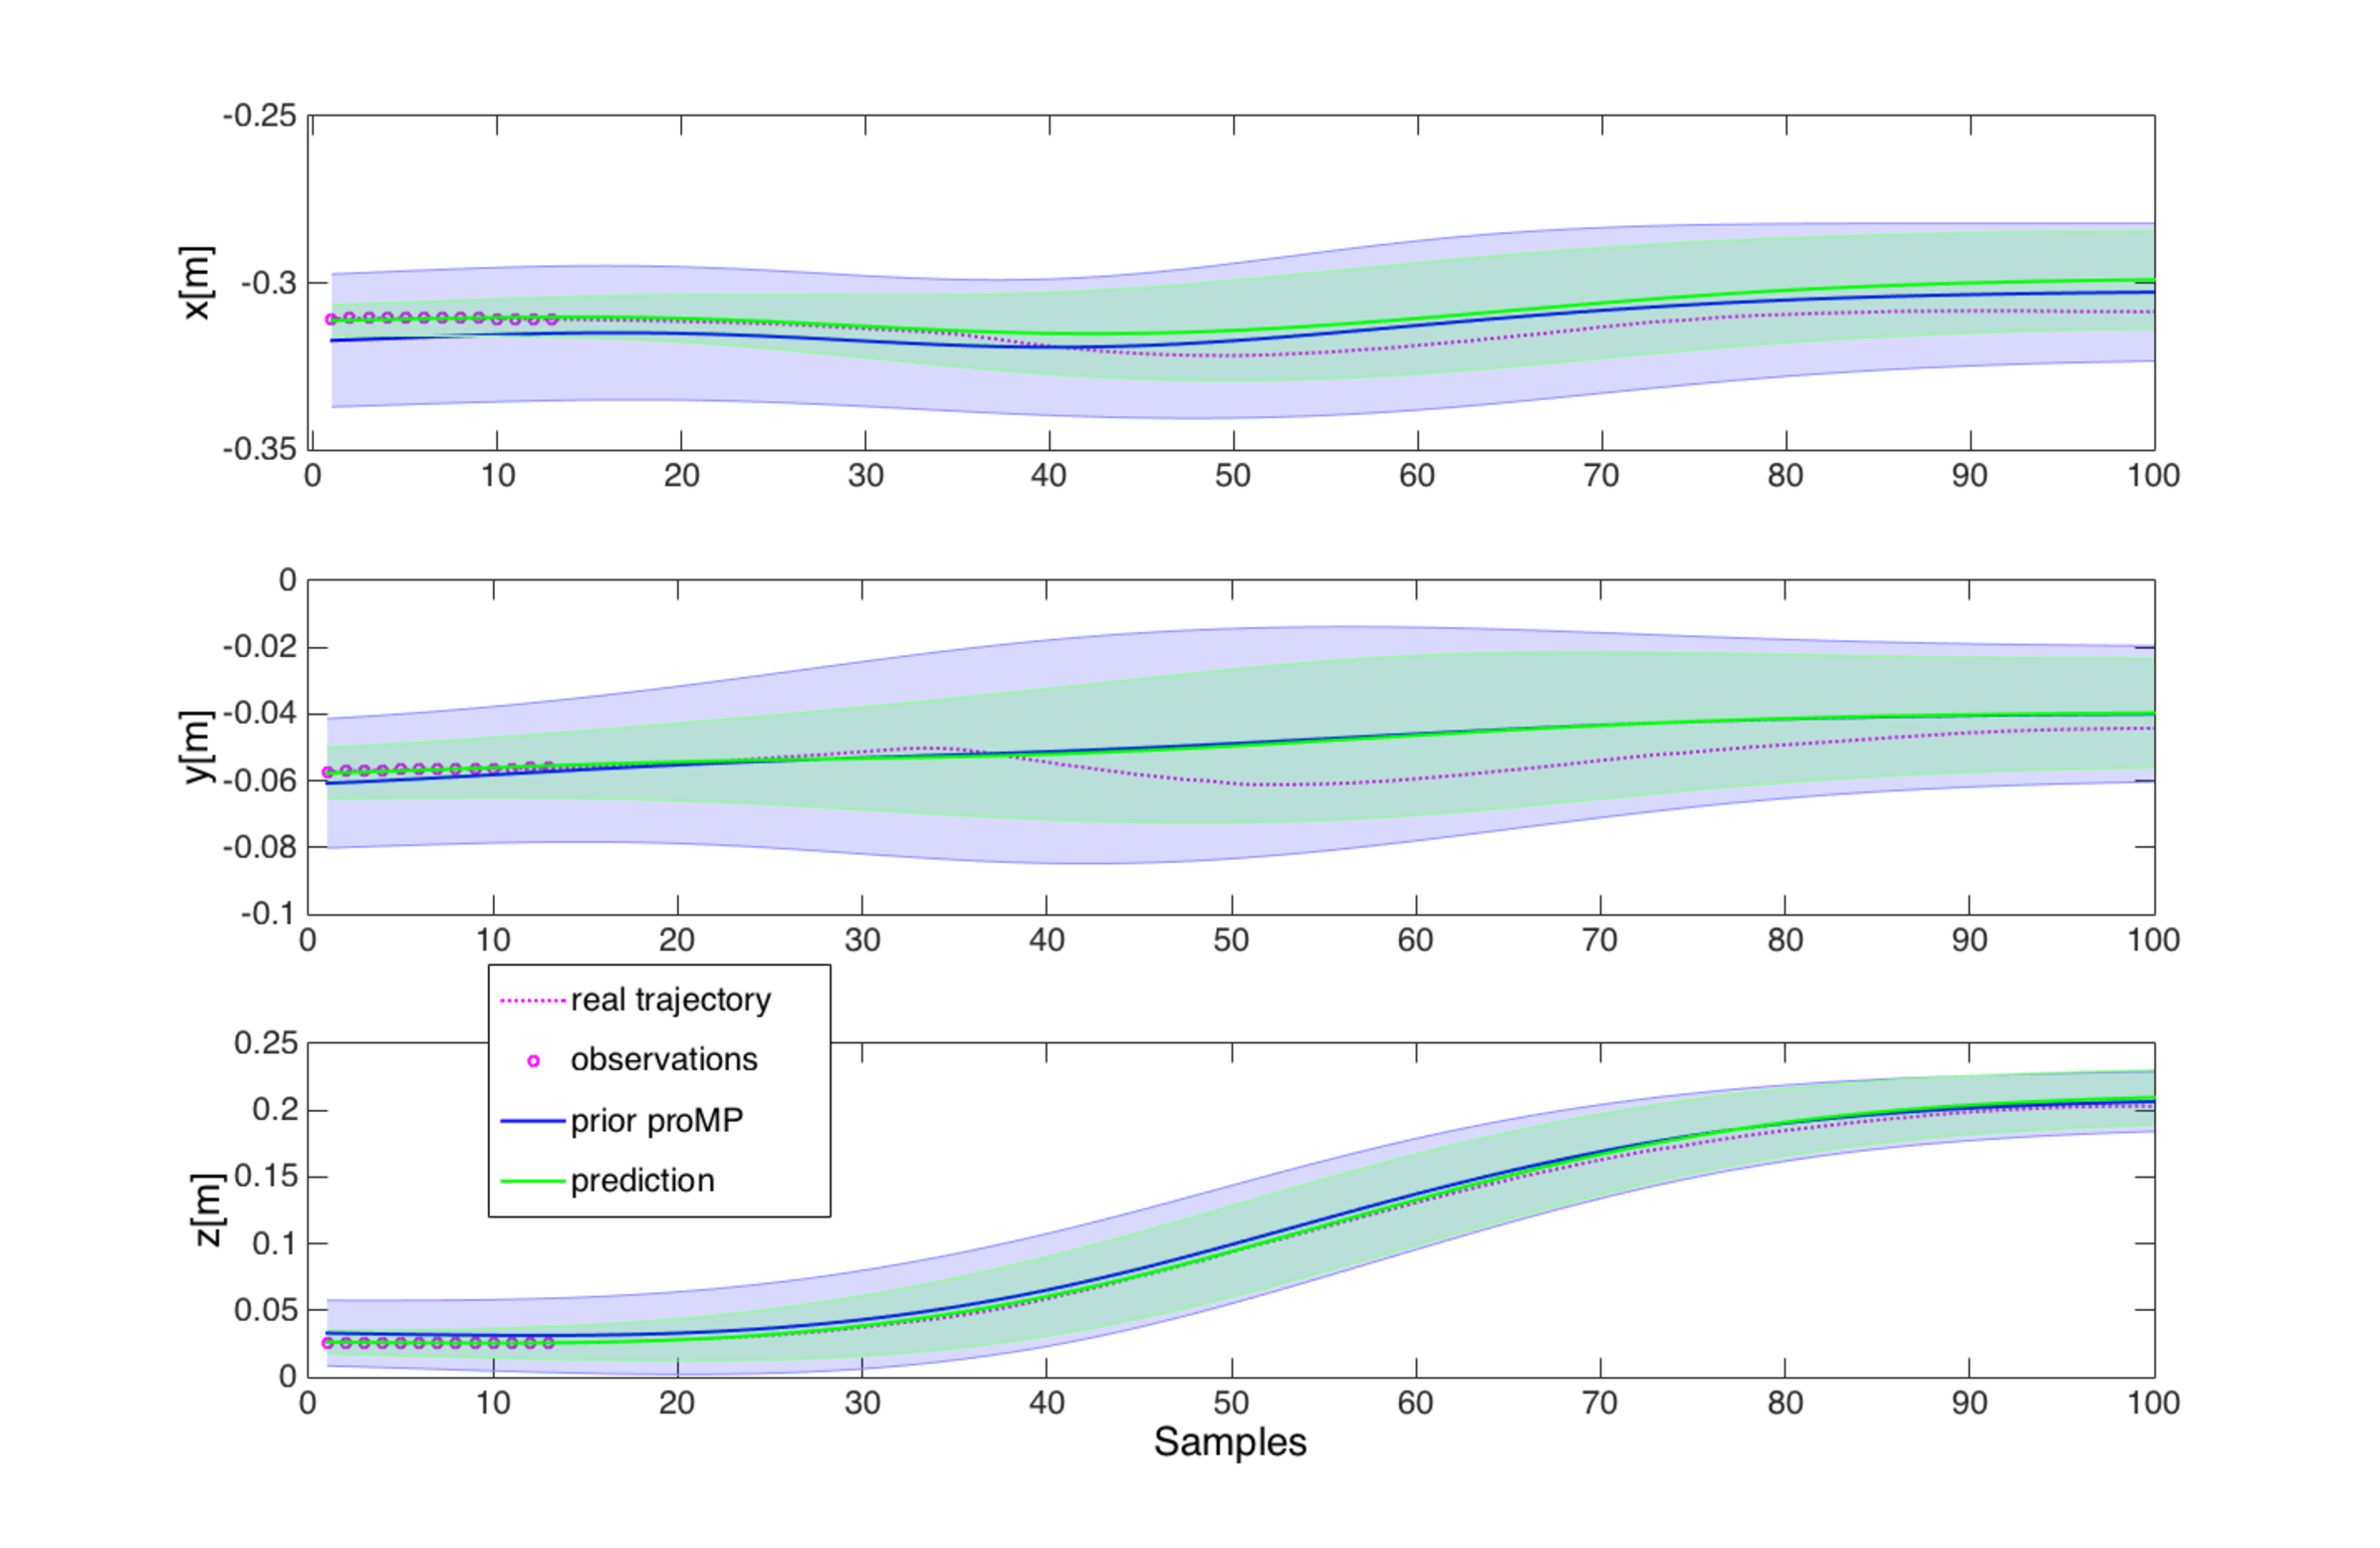
\includegraphics[height=11cm]{img/liftingWgeomagic/INFERENCE2.pdf}
%\caption{Prediction of the future trajectory, after $n_o=15$ observations, given the prior ProMP learned from $n$ demonstrations.}\todo{$/*$update the figure$*/$}
%\label{fig:predictionLifting15}
%\end{figure}

\subsection{Prédiction du paramètre de modulation du temps de la trajectoire}\label{sec:predictDuration}
Dans la section précédente, la formulation générale des \textit{ProMPs}a été présentée, en faisant l'hypothèse que toutes les trajectoires observées étaient même durée et donc qu'elles sont représentées par le même nombre d'échantillons.\footnote{Actually, we call here duration what is in fact the total number of samples for the trajectory.}
C'est pourquoi la durée des trajectoires générés par les \textit{RBFs} est fixe et égale à $\bar{s}$. 

Cependant, afin de pouvoir générer des trajectoires dans des conditions expérimentales réelles, on considère maintenant que la durée de ces trajectoires de démonstration varie.
Dans ce but, un paramètre de modulation du temps $\alpha$ est introduit permettant de redimensionner la trajectoire actuelle afin qu'elle ne soit plus définie par $t_{f}$ mesures mais par $\bar{s}$: $\alpha = \bar{s} / t_{f}$.
%This variable rescales the \textit{RBFs} of the model to the trajectory duration. 
%It relies on the trajectory duration and a reference number of samples $\bar{s}$.
La durée normalisée $\bar{s}$ peut être choisi arbitrairement; par exemple, elle peut correspondre à la moyenne des durées des trajectoires, \textit{e.g.}, $\bar{s}=moyenne(t_{f1},\ldots,t_{fK})$.
% (we have one sample per iteration time $t$).
Dans la littérature, ce terme $\alpha$ est parfois appelé la \textit{phase}~\cite{paraschos2013probabilistic,paraschos2013probabilisticTrajectory}. 
\toimprove{Ce terme $\alpha$ change la phase des \textit{RBFs}, foncitions qui sont étalée temporellement sur l'ensemble de la durée de la trajectoire}.

Le paramètre de modulation du temps de la $i^e$ trajectoire $\Xi_i$ est calculé avec : $ \alpha_i = {\bar{s} \over t_{fi}}$. Ainsi, on obtient : $\alpha \cdot t \in [1:\bar{s}]$. Ainsi, le modèle \textit{ProMP} amélioré devient :
\begin{eqnarray}
\xi_t = \Phi_{\alpha t} \boldsymbol{\omega} + \epsilon_t \, ,
\end{eqnarray}
où $\Phi_{\alpha t}$ est la matrice de \textit{RBFs} évaluée au temps $\alpha t$. L'ensemble des $M$ fonctions Gaussiennes représentant les \textit{RBFs}sont étalée pour représenter le même nombre d'échantillons $\bar{s}$. Ainsi, on obtient :
$$ \Phi_{\alpha t}=[\psi_{1}(\alpha t), \psi_{2}(\alpha t), \ldots., \psi_{M}(\alpha t)].$$
%\begin{equation}
%\Phi_{\alpha t}=[\psi_{1}(\alpha t), \psi_{2}(\alpha t), \ldots., \psi_{M}(\alpha t)] \mathrm{,~with:}  
%\psi_{i}(\alpha t) = {1 \over\sum_{j=1}^M \psi_{j}(\alpha t) }exp\{{-({\alpha t / \bar{s}} - c(i))^2 \over {2h}}\} 
%\end{equation}

%The Matlab function that allows to create such \textit{RBFs} is
%
%\mcode{Phi_alpha = computeBasisFunction (s_ref,M, D, alpha, t_f, c, h,no)}
%
%\todo{Pourquoi parler ici de code???????? C est dans les sections suivantes, pas ici!!!}
%
%\begin{itemize}
%\item \mcode{s_ref} = $\bar{s}$: the reference number of samples;
%\item $M$ is the number of Gaussians of the \textit{RBFs};
%\item $D$ is the $\xi_t$ dimension;
%\item \mcode{alpha} is the time modulation parameter of $\Xi$;
%\item \mcode{t_f = s_ref / alpha} is the total time duration of $\Xi$; 
%\item \mcode{c} and \mcode{h} are the parameters of the Gaussians; 
%\item \mcode{no} informs the data number that we want to model by the \textit{RBFs} (here $[1:no]$).
%\end{itemize} 
%
%The output matrix \mcode{Phi_alpha} $= \Phi_{\alpha [1:no]}$ is the \textit{RBF} matrix computed to represent the first $n_o$ observed data points of a $\Xi$ trajectory.

Durant la phase d'apprentissage, un ensemble de paramètres $\alpha$ est appris : $S_{\alpha} = \{\alpha_{1},\ldots,\alpha_{n}\}$.
Puis, en utilisant ce set, la \textit{ProMP} apprise peut être rejouée à différentes vitesses. Par défaut, (\textit{e.g.} quand $\alpha=1$), la vitesse de la trajectoire permet de finir le mouvement en $\bar{s}$ itérations.


\begin{figure}[h!]
\centering
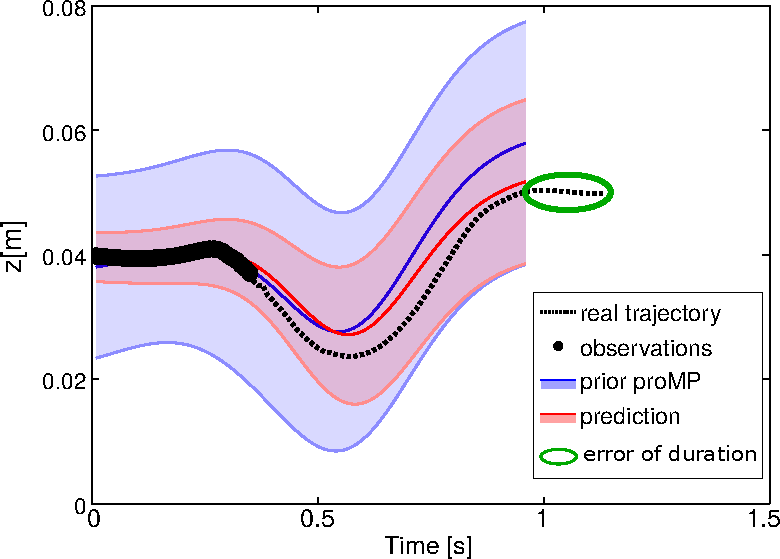
\includegraphics[width=13cm]{img/mean_alpha_errV2.pdf}
\caption{Trajectoire prédite à partir de l'observation d'une trajectoire initiée (points noirs); réalité terrain (\textit{e.g.}, la trajectoire que l'utilisateur voudrait que le robot execute) ; distribution à priori (en bleu clair) ; et distribution postérieur (en rouge), calculée en \toimprove{conditionnant} la distribution afin qu'elle corresponde aux observations. Ici, le calcul de la distribution postérieur est uniquement calculée à partir de la moyenne $\alpha$, de l'ensemble $\alpha_1, \ldots, \alpha_K$ correspondant aux $K$ trajectoires de démonstrations. Sans prédiction du paramètre de modulation du temps de la trajectoire observée et donc en utilisant la moyenne $\alpha$, la trajectoire prédite a une durée visiblement différente de la réalité terrain.}

\label{fig:moyenneAlpha}
\end{figure}

Durant l'inférence, le paramètre de modulation du temps $\alpha$ de la trajectoire observée partiellement n'est pas connu. À moins que ce paramètre soit fixé à priori, le robot doit alors l'estimer. Cette estimation est essentiel pour assurer une bonne reconnaissance, comme cela est montré dans la Figure~\ref{fig:moyenneAlpha} : la trajectoire inférée (représentée par la moyenne de la distribution postérieure en rouge) 
%\todo{why "has not the same" is not correct?} 
%For Oriane: check https://english.stackexchange.com/questions/13672/have-not-versus-do-not-have
n'a pas la même durée que la trajectoire attendue ``réelle'' (qui correspond à la réalité terrain). Cette différence est du à l'erreur d'estimation du paramètre de modulation du temps. Cette estimation $\hat{\alpha}$  est calculée par défaut en tant que moyenne de l'ensemble des paramètres $\alpha_k$ calculés lors de la phase d'apprentissage :
\begin{equation}
\label{eq:avg}
%\hat{\alpha} = {1 \over |S_{\alpha k}|} \sum_{\alpha \in S_{\alpha k}} \alpha
\hat{\alpha} = {{\sum \alpha_k} \over n_k} .
\end{equation}

Cependant, l'utilisation de la valeur moyenne du temps de modulation est appropriée uniquement lorsque la primitive représente des mouvements dirigés vers un but très régulier, ou plus généralement lorsqu'il est raisonnable de supposer que les différences de vitesse entre les trajectoires peuvent être négligé (ce qui n'est pas le cas en général). Ainsi, pour beaucoup d'applications, cette estimation est trop imprécise.

C'est pourquoi nous avons trouvé un moyen d'estimer la durée des trajectoires observées, ce qui correspond à estimer de manière précise le paramètre de modulation du temps $\hat{\alpha}$.
Afin d'estimer $\hat{\alpha}$, on a implémenté différentes méthodes.
%Instead, we implemented simpler methods that select the most likely $\hat{\alpha}$ temporal modulation parameter according to different methods.
%\begin{itemize}
%\label{itemize:methodAlphaEstimation}
La première méthode consiste au calcul de la \textbf{moyenne des $\alpha_k$}, comme montré dans l'Équation \ref{eq:avg}. La seconde méthode consiste au calcul du \textbf{maximum de ressemblance }
%As first method, we can simply use the \textbf{moyenne of the $\alpha$}:
%\begin{equation}
%\label{eq:avg}
%%\hat{\alpha} = {1 \over |S_{\alpha k}|} \sum_{\alpha \in S_{\alpha k}} \alpha
%\hat{\alpha} = {{\sum \alpha_k} \over K} .
%\end{equation}
avec :
\begin{equation}
\label{eq:ml}
\hat{\alpha} = \mathrm{argmax}_{\alpha \in S_{\alpha k}}\{\mathrm{loglikelihood}(\Xi^o,\mu_{\boldsymbol{\omega}_k}, \sigma_{\boldsymbol{\omega}_k}, \alpha_k)\} .
\end{equation} 
La troisième méthode consiste au critère de \textbf{distance minimum}, qui consiste à rechercher le meilleur $\hat{\alpha}$ qui minimise les différences entre la trajectoire observée  $\Xi^o_t$ et celle prédite pour les $n_o$ premières itérations :
\begin{equation}
\label{eq:minDist}
\hat{\alpha} =\mathrm{argmin}_{\alpha \in S_{\alpha k}} \{\sum_{t=1}^{{n_o}} |\Xi^o_t - \Phi_{\alpha t} \mu_{\boldsymbol{\omega}_k}|\} .
\end{equation} 
La quatrième méthode consiste en la création d'un \textbf{modèle}, 
% \todo{find another name}: -> why changing it? the reviewers didnt mind that
basé sur la supposition qu'il y ait une corrélation entre $\alpha$ et la ``variation'' de la trajectoire $\delta_{n_o}$  entre le début et le temps $n_o$. Cette ``variation'' $\delta_{n_o}$ peut correspondre au calcul de la variation positionnelle, \textit{e.g.}, $\delta_{n_o} = X(n_o) - X(1)$,  ou au calcul de la variation de l'ensemble des données représentant la trajectoire, $ \delta_{n_o} =\Xi(n_o) - \Xi(1)$, \toimprove{ou encore n'importe laquelle de ces mesures, tant que l'hypothèse est approprié au type de trajectoire.}\footnote{\toimprove{Dans notre cas, cette hypothèse est appropriée puisque les trajectoires dirigées vers un but de notre application croient généralement de manière monotomne.} }
En effet, le paramètre $\alpha$ peut être lié à la vitesse de mouvement, qui peut être approximée de manière \toimprove{brut} par $\dot{X} ={ \delta X  \over t_f}$ ($\dot{\Xi} ={ \delta \Xi  \over t_f}$). Nous modelisons le réechantillonage entre $\delta_{n_o}$ et $\alpha$ avec : 
\begin{equation}
\label{eq:model}
\alpha = \Psi(\delta_{n_o})^\top \boldsymbol{\omega}_\alpha + \epsilon_\alpha,
\end{equation} 
où $\Psi$ correspond à la matrice de \textit{RBFs}, et $\epsilon_\alpha$ au bruit suivant une loi normale centrée \todo{et réduite ?} .
Lors de la phase d'apprentissage, le paramètre $\boldsymbol{\omega}_\alpha$ est calculé en utilisant l’Équation~\ref{eq:w}. 
Lors de la phase de prédiction, le paramètre $\hat{\alpha} = \Psi(\delta_{n_o})^\top \boldsymbol{\omega}_\alpha$ est calculé.
%\end{itemize}

Une étude test, présentée dans la Section~\ref{sec:simulatedTimeModulationModels}, met en jeu le iCub simulé et permet de comparer ces quatre méthodes d'estimation du paramètre  $\alpha$.

\todo{verif déja inclu dans SOA}
Dans la littérature, il existe d'autres méthodes permettant de calculer ce paramètre $\alpha$. Par exemple~ \cite{ewerton2015learning} propose une méthode qui modélise localement la variabilité de la vitesse d'execution des trajectoires. Dans~\cite{maeda2016probabilistic} ils utilisent une méthode qui permet d'améliorer la méthode \textit{Dynamic Time Warping} en imposant une fonction régulière sur l’alignement temporaire, à l'aide d'optimisation locale. Ces méthodes seront implémentées dans les futures études.
%In this software, we did not implement such methods yet, since the four proposed criteria are simpler.


\subsection{\toimprove{Reconnaître une primitive de mouvement parmi plusieurs}}
\label{sec:ManyProMP}
%
%we learn many movement primitives which correspond to different tasks.\\
%Let  $S_k = \{\Xi_1,\ldots, \Xi_n\}_k$, the set of trajectories that correspond to the $k$-th movement primitive.
%Let recall that $\Xi_i = [\xi_{1} \ldots \xi_{t_{fi}}]^\top$ is the $i$-th trajectory of this data set, where $t_{fi}$ is the final time of the movement. 
%
Pour rendre les robots performant, ceux-ci doivent être capable de proposer différents comportements afin d'effectuer différentes tâches.  Dans notre logiciel, chaque \textit{ProMP} représente une tâche distincte.
Ainsi, il est important que le robot soit capable d'apprendre différentes \textit{ProMPs}, disons $K$, puis d'être capable de reconnaître laquelle de ces trajectoire est initiée par l'utilisateur du robot.
%We are also interested in learning many ProMPs, say $K$ ProMPs.

Durant la phase d'apprentissage d'une Primitive de Mouvement $k \in [1:K]$,  le robot observe différentes trajectoires $S_k = \{\Xi_1,\ldots,\Xi_n\}$. Pour chaque \textit{ProMP}, il apprend alors une distribution à partir de l'ensemble des vecteurs paramètres  $p(\boldsymbol{\omega}) \sim \mathcal{N}(\mu_{\boldsymbol{\omega}_k}, \Sigma_{\boldsymbol{\omega}_k})$, à l'aide de l'Équation~\ref{eq:w}. De plus, le robot enregistre les différentes durées des trajectoires observées : $ S_{\alpha k} = \{\alpha_{1k},\ldots,\alpha_{nk}\}$.

Après avoir apris ces $K$ \textit{ProMPs}, le robot peut utiliser les informations apprises afin d’exécuter une trajectoire et sa tâche correspondante. Pour cela, le robot doit d'abord être capable de reconnaître, à partir des observations partielles de la trajectoire initiée par l'utilisateur, quel est le mouvement et la tâche attendue, puis comment la continuer.
%\todo{why not: has to?} must finish a human-initiated movement on its own. 

Soit $\Xi^{o} = [\Xi_1 \ldots \Xi_{n_o}]^\top$ les observations partielles de la trajectoire initiée.
À partir de ces observations partielles, le robot peut reconnaître la \textit{ProMP} ``correcte'' (\textit{e.g.}, la plus probable) $\hat{k} \in [1:K]$ en suivant plusieurs étapes.
% by:
%\begin{itemize}
Tout d'abord, pour chaque \textit{ProMP} $k \in [1:K]$, le robot commence par calculer le paramètre de modulation de temps $\hat{\alpha}_k$ le plus probable (\textit{c.f.} Section~\ref{sec:predictDuration}), afin d'obtenir un ensemble contenant les \textit{ProMPs} couplées avec leur durée la plus probable : $S_{[\mu_{\boldsymbol{\omega}_k}, \hat{\alpha}_k]} = \{(\mu_{\boldsymbol{\omega}_1},\hat{\alpha}_1),\ldots,(\mu_{\boldsymbol{\omega}_K},\hat{\alpha}_K)\}$

Puis, le robot calcul la \textit{ProMP} $\hat{k}$ la plus probable depuis l'ensemble : $S_{[\mu_{\boldsymbol{\omega}_k}, \hat{\alpha}_k]}$, en utilisant différents critères. \todo{?}
Afin de minimiser la distance entre les observations partielles et la moyenne des premières données de la \textit{ProMP}, le robot peut calculer :
\begin{equation} \label{eq:mostlikelypromp}
\hat{k} = \arg \min_{k \in [1:K]} \,   \left[      {1 \over n_o} \sum_{t=1}^{n_o}| \Xi_{t} - \Phi_{\hat{\alpha}_k t} \, \mu_{\boldsymbol{\omega}_k} | \right]
\end{equation}
Dans l'Équation~\ref{eq:mostlikelypromp}, pour chaque \textit{ProMP}  $k \in [1:K]$, la distance moyenne est calculée entre la trajectoire initiée $\Xi_t$  et la moyenne de la \textit{ProMP} $\Phi_{\hat{\alpha}_k t} \mu_{\omega_k}$, avec $t = [1:n_o]$.
La \textit{ProMP} $\hat{k}$ la plus vraissemblable est alors selectionnée en calculant la distance minimum (arg min). D'autres méthodes sont possibles pour calculer la \textit{ProMP} la plus probable, méthodes inspirées par celles présentées pour l'estimation du paramètre de modulation du temps ( \textit{c.f.} Section précédente). C'est à dire, l'estimation à l'aide du maximum de vraisemblance ou en apprenant une modélisation du paramètre, \toimprove{modèle basée sur des données de la trajectoire}.

%\end{itemize}
%\todo{EXPLAIN THIS EQUATION}

%Now the ProMP the most similar to the early-trajectory is identified, we can update the $\hat{k}$-th ProMP to adapt it to the observed early-trajectory.

Lorsque la $\hat{k^e}$ \textit{ProMP} la plus probable a été identifiée, la distribution postérieure de cette \textit{ProMP} est caclulée afin de prendre en compte la portion initiale de la trajectoire observée, en utilisant l'Équation~\ref{eq:inf}:

%The first step is then to compute $\hat{t_f}$ \rev{(the expected duration of the trajectory)} by: 
%\begin{equation}
%\hat{t_f} = \hat{\alpha_{\hat{k}}} \times \bar{s}
%\end{equation}
%The second step consists of updating the ProMP to match the early observations, using Equation~\ref{eq:inf}:

%\hat{\alpha}_{\hat{k}}
%\omega}_{\hat{k}}
\begin{equation} \label{eq:udateWithAlpha}
\left\{
\begin{array}{rl}
\hat{\mu}_{\boldsymbol{\omega}_{\hat{k}}} &= \mu_{\boldsymbol{\omega}_{\hat{k}}}  + K(\Xi^o - \Phi_{\hat{\alpha}_{\hat{k}}[1:{n_o}]}\mu_{\boldsymbol{\omega}_{\hat{k}}} ) \\ 
\hat{\Sigma}_{\boldsymbol{\omega}_{\hat{k}}}  &= \Sigma_{\boldsymbol{\omega}_{\hat{k}}}  - K(\Phi_{\hat{\alpha}_{\hat{k}}[1:{n_o}]} \Sigma_{\boldsymbol{\omega}_{\hat{k}}} ) \\
K&= \Sigma_{\boldsymbol{\omega}_{\hat{k}}} \, \Phi_{\hat{\alpha}_{\hat{k}}[1:{n_o}]}^\top \, (\Sigma_{\xi^o} + \Phi_{\hat{\alpha}_{\hat{k}}[1:n_o]}\Sigma_{\boldsymbol{\omega}_{\hat{k}}}  \Phi_{\hat{\alpha}_{\hat{k}}[1:n_o]}^\top)^{-1}
\end{array}
\right.
\end{equation}
avec $\hat{\alpha}_{\hat{k}}[1:n_o] = \hat{\alpha}_{\hat{k}} \, t$ (forme matricielle), avec $t \in [1:n_o]$.

Finalement, la trajectoire inférée est calculée avec : 
$$\forall t \in [1:\hat{t}_f], \hat{\xi}(t) = \Phi_t \, \hat{\mu}_{\boldsymbol{\omega}_{\hat{k}}}$$
avec une estimation de la durée de la trajectoire correspondant à : $\hat{t}_f = \hat{\alpha}_k\bar{s}$.
Le robot est alors capable de finir le mouvement en executant la trajectoire ``future'' la plus probable : $\hat{\Xi} =[\hat{\xi}_{n_o+1} \ldots \hat{\xi}_{\hat{t_{f}}}]^\top$.


%\newpage
%%%%%%%%%%%%%%%%%%%%%%%%%%%%%%%%%%%%%%%%%%%%%%%%%%%%%%%%%%%%%%%%%%%%%%%%%%%%%%%%
\section{Présentation du logiciel}\label{sec:softwareOverview}

Dans cette Section, le logiciel libre d'accès est présentée. Ce logiciel est composé de deux modules, représentés dans la Figure \ref{fig:orgaSoftware}.

\label{sec:software}
\begin{figure}[h]
\center
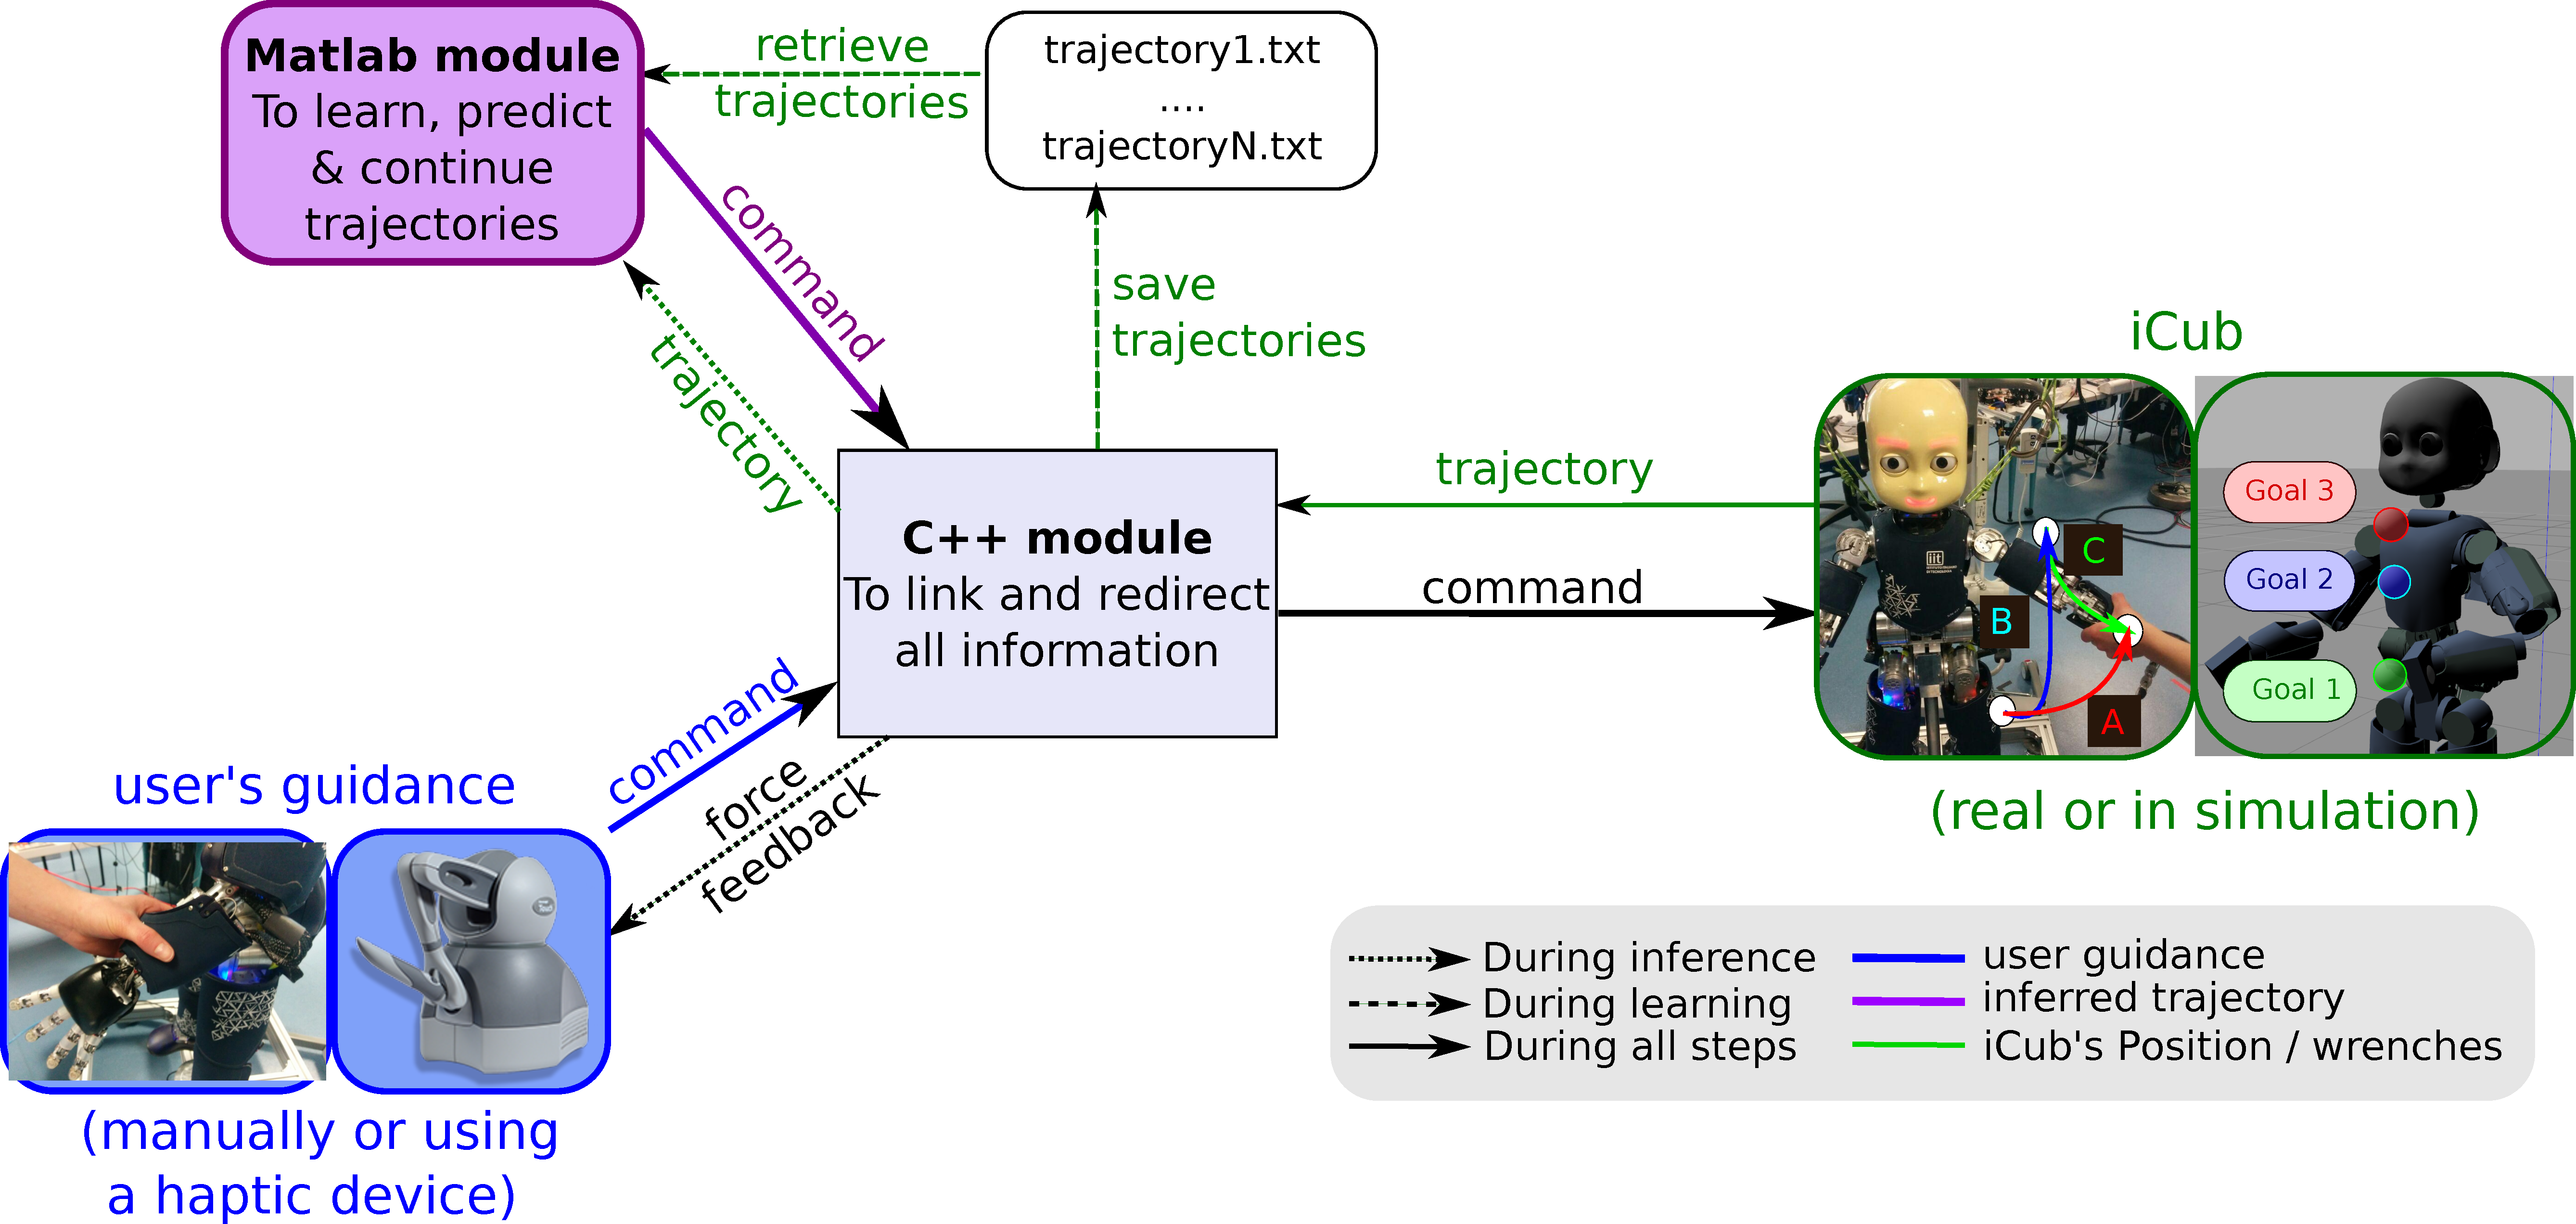
\includegraphics[width=\hsize]{img/liaisonAllProgramV3.pdf}
\caption{Architecture du logiciel avec représentation des échanges de donées.\\ Le contrôle du robot est soit guidé par son utilisateur (manuellement ou à l'aide d'un dispositif haptique) représenté en bleu, ou à l'aide d'un module Matlab, présenté en violet. \toimprove{Le module  C++ permet de faire passer l'information de contrôle à la commande robotique, comme présenté en noir}. De plus, ce module transmet l'information qui provient du iCub.}
\label{fig:orgaSoftware}
\end{figure}

Durant la phase d'apprentissage, où le robot apprend les différentes \textit{ProMPs} et leur tâche correspondante, le robot est contrôlé par un utilisateur. Celui-ci peut guider le robot manuellement, lorsqu'il s'agit du iCub réel, ou à l'aide d'un dispositif haptique lorsqu'il s'agit de la simulation du robot.

Un module Matlab permet de rejouer les \textit{ProMPs}, ou de finir un mouvement qui a été initié par son utilisateur. Ce module permet au robot d'apprendre des \textit{ProMPs} à partir des trajectoires effectuées; de rejouer ces \textit{ProMPs}; de reconnaître la \textit{ProMP} qui correspond le plus à une trajectoire en cours; et de prédire le ``futur'' de cette trajectoire, jusqu'à atteindre le but.
%\todo{and to make sure that the user's forces exerted on the robot are not stronger than the ones learnt.}

Un module C++ transmet au robot l'information de contrôle qui provient soit de l'utilisateur, soit du module Matlab. Le robot est alors capable de finaliser le mouvement inité par son utilisateur (directement ou à l'aide d'un dispositif haptique) de manière autonome, comme présenté dans la Figure~\ref{fig:conceptProMP}. %\todo{This program communication also allows to correct the robot behaviour if the users forces are stronger than the expected ones.} \\
Le module C++ est présenté dans la Section~\ref{subec:Setup}, puis une explication théorique des algorithmes utilisés dans le module Matlab  est donnée dans la Section~\ref{sec:theory}. Un guide permettant d'utiliser ce module Matlab est d'abord présenté dans  la Section~\ref{sec:example1DOF} dans le cas d'un exemple jouet, puis dans la Section~\ref{sec:3ProMPsAppli} dans le cas de notre application, où le robot simulé apprend différentes données sur les mouvements (\textit{e.g.}, il s'agit de \textit{ProMPs} à plus haute dimension). Finalement, les résultats de l'application effectué sur le réel robot iCub sont présentés dans la Section~\ref{sec:appliRealIcub}.

Notre logiciel est disponible avec une licence GPL, et est accessible publiquement à l'adresse : 

\url{https://github.com/inria-larsen/icubLearningTrajectories}.

Ce répertoire propose à la fois un tutoriel, un fichier d'explication (README) et des vidéos de présentation.
Le fichier d'explication décrit comment lancer des démonstrations basiques. Les vidéos présentent ces démonstrations, afin d'éclaircir le fonctionnement de cette application. Les sections prochaines détaillerons tout d'abord comment fonctionne le ``programme de démonstration'' disponible, permettant l'apprentissage d'une primitive à une dimension; suivi par la présentation d'une application spécifique au iCub (d'abord en simulation puis sur le robot réel).
%\todo{check that, it is not in the readme??}


%%%%%%%%%%%%%%%%%%%%%%%%%%%%%%%%%%%%%%%%%%%%%%%%%%%%%%%%%%%%%%%%%%%%%%%%%%%%%%%%
\section{Exemple fournis par le logiciel : apprentissage d'une primitive à une dimension}
\label{sec:example1DOF}
Cette section présente comment utiliser le logiciel afin d'apprendre une \textit{ProMP} à une dimension. Cette exemple nécessite uniquement l’utilisation du dossier \textit{MatlabProgram}, composé de :
\begin{itemize}
\item Un sous dossier nommé  ``Data'', où un ensemble de trajectoire permet d'apprendre des \textit{ProMPs}. Ces trajectoires sont enregistrées dans des fichier textes, contenant les informations suivantes :
%that
%\sout{there are some samples of trajectories in text files. These text files} }can be organize in various ways:
\begin{itemize}
\item [-] \textbf{paramètres d'entrée }: \# e$_1$ \# e$_2$ [...]
\item [-] \textbf{paramètre d'entrée avec information temporelle}: \# temps \# e$_1$ \# e$_2$ [...]
\item [-] programme d'enregistrement de trajectoire \textbf{\textit{recordTrajectories.cpp}}: \textit{c.f.} Section~\ref{sec:dataAquisition} pour plus d'information.
\end{itemize}
\item Un sous dossier nommé ``used\_functions''. Celui-ci contient toutes les fonctions utilisées permettant de récupérer les trajectoires, de calculer les \textit{ProMPs}, d'inférer les trajectoires, ainsi que de représenter les résultats dans des figures. L'utilisation de ce logiciel ne nécessite pas la compréhension de l'ensemble de ces fonctions. 
%\sout{the use of this toolbox doesn't require to understand these functions}}. 
Au début de ces fonctions, des lignes expliquent leur fonctionnement et précisent à quoi correspondent les paramètres d'entrée et de sortie.
\item Des scripts Matlab dénommés ``demo\_*.m". Il s'agit d'exemples basiques permettant de comprendre comment utiliser ce logiciel.
\end{itemize}

Le script \mcode{demo\_plot1DOF.m} permet de calculer une \textit{ProMP} et de continuer un mouvement qui a été initié. La \textit{ProMP} est calculée à partir d'un ensemble de trajectoires récupéré d'un fichier ".mat", appelé \textit{traj1\_1DOF.mat}. Dans ce script, les variables sont d'abord définies afin de correspondre à l'ensemble des trajectoires :
\begin{tabular}{|c|l|}
  \hline
  \textbf{Assignation de la variable } & \textbf{Commentaire}\\
  \hline
  DataPath\= 'Data\/traj1\_1DOF.mat'; & Peut correspondre à un fichier ".mat" ou ".txt". Dans la démonstration courante, vous pouvez aussi écrire\\
  & DataPath $=$ 'Data/traj1' si vous souhaitez utiliser les fichiers textes de cet ensemble de données.\\
     \hline
  typeRecover= '.mat' & Ou .txt, selon le choix du type de fichier de données.\\
    \hline
  inputName = {'z[m]'}; & Étiquette des données d'entrée des trajectoires. Ici, $z$ représente la coordonnée Cartésienne d'axe $z$.\\
    \hline
  s\_ref=100; & Nombre d'échantillons utilisé en tant que référence afin de re-échantillonner l'ensemble des trajectoires pour qu'elles aient la même longueur temporelle.\\
    \hline
  nbInput = 1; & Dimension du vecteur paramètre contenant les mesures représentant les trajectoires.\\
    \hline
  M = 5;  & Nombre des fonctions à base radiale par donnée d'entrée 
  .\\
    \hline
  expNoise = 0.00001;  & \toimprove{bruit estimé sur les mesures de la trajectoire}.\\
    \hline
  percentData = 20;  & Pourcentage des données observées avant l'inférence.\\
  \hline
  \end{tabular}

Dans ces variables, il y a :

\begin{itemize}
\item \mcode{DataPath} est le chemin d'accès menant aux données enregistrées. Si les données sont enregistrées dans des fichiers textes, cette variable contient le nom du dossier où les fichiers textes sont enregistrés. Ces fichiers textes sont appelés ``record$X$.txt", avec $X \in [0:n-1]$ si ils sont $n$ trajectoires. Un dossier est utilisé pour apprendre une \textit{ProMP}. Si les données sont déjà contenues dans un fichier ``.mat", le chemin d'accès total doit être inscrit, avec l'extension. Les données dans le fichier ``.mat" coïncident avec les données de sortie de la fonction Matlab \mcode{loadTrajectory}. %, presented in Figure~\ref{fig:yobject}.
\item \mcode{nbInput}= $D$ correspond à la dimension du vecteur d'entrée $\xi_t$. 
%This variable can be divided in two to precise in \mcode{nbInput(1)} what are the first $\xi_t$  dimensions used to recognize both the correct movement primitive and the time modulation of the initiated trajectory. In that case, \mcode{nbInput(2)}$= D - $\mcode{nbInput(1)}, contains the other dimensions, only used to compute the posterior distribution.
\item \mcode{expNoise} $= \Sigma^o_\xi$ correspond au bruit estimé des mesures de la trajectoire initiée. Plus cette variable est petite, plus la modification de la \textit{ProMP} va être importante, afin de correspondre plus précisément aux observations.
\end{itemize}

%\rev{After this variable declaration, the user can just launch the script. To give a deeper understanding of this script, we now detail which and how functions are called in it.} 
Le script va maintenant être détaillé. Afin de récupérer les données enregistrées dans le fichier ``.txt'', la fonction suivante est appellée :

\mcode{t\{1\} = loadTrajectory(PATH, nameT, varargin)} 

Ces paramètres d'entrée précisent le chemin d'accès des données enregistrées, ainsi que l'étiquette représentant le type de trajectoire. D'autres informations peuvent être ajoutées, à l'aide de la variable \mcode{varargin} (\textit{c.f.}, informations commentées en tête de cette fonction). 
%For more detail about these parameters, read the beginning of this function. 
Les paramètres de sortie de cette fonction correspond à un objet contenant toutes les informations des trajectoires de démonstrations. Ces paramètres sont le nombre de trajectoires \mcode{nbTraj} ; le nombre d'itérations de cette simulation \mcode{realTime} ; l'ensemble des vecteurs (et matrices) représentant les trajectoires \mcode{y} (et \mcode{yMat}) ; \textit{etc.}. 
%\rev{\sout{Note that to simplify the Matlab's notation, we denote the $\Xi$ trajectory by \mcode{y} (or \mcode{yMat} in all the toolbox functions}}. 
Ainsi, \mcode{t\{1\}.y\{i\}} contient la $i^e$ trajectoire.

%\begin{figure}[h]
%\centering
%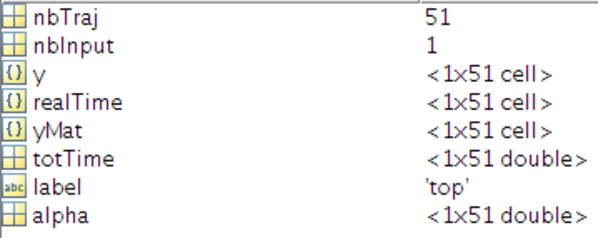
\includegraphics[height=4cm]{img/yobject.pdf}
%\caption{Object that contains information about 51 observed trajectories of a 1DOF movement primitive.}
%\label{fig:yobject}
%\end{figure}

La fonction Matlab \mcode{drawRecoverData(t\{1\}, inputName,'namFig', nFig, varargin)} permet d'afficher sur une figure (numéroté \mcode{nFig}) les mesures des trajectoires récupérées. %By lack of place, we don't represent here these trajectories.
Un exemple est montre dans la Figure~\ref{fig:1DOFtrajectoriesProMP}, sur la gauche. Les différentes durées de trajectoires y sont visibles : en moyenne, cette durée est de $1.17 \pm 0.42$ secondes.

% a plot such as Figure~\ref{fig:1DOFtrajectories}. In this Figure, the average duration of these trajectories is $1.17 \pm 0.42$ seconds.

%\begin{figure}[h]
%\centering
%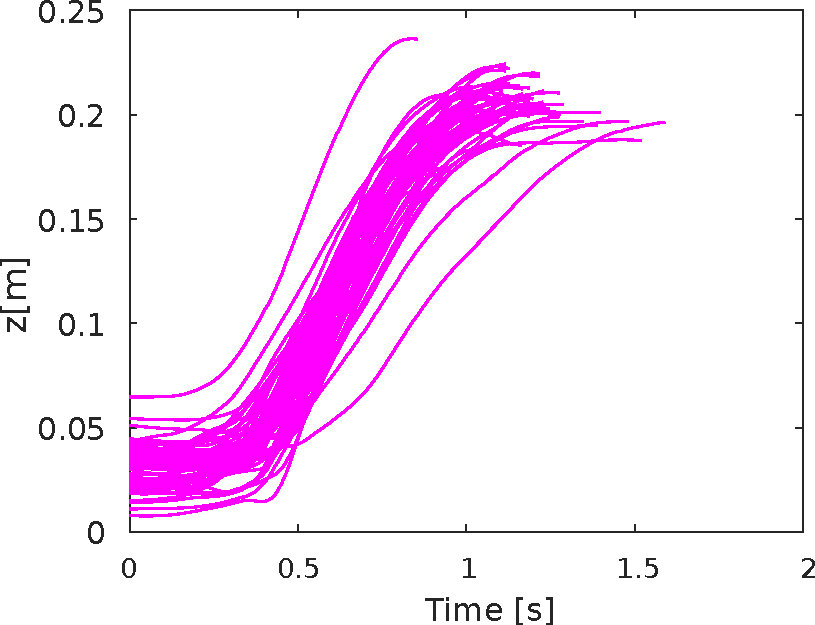
\includegraphics[height=8cm]{img/1DOFtrajectoriesV2.pdf}
%\caption{The trajectories of the test dataset for 1DOF primitive.}
%\label{fig:1DOFtrajectories}
%\end{figure}
De cet ensemble de trajectoires de démonstration \mcode{t\{1\}}, un sous ensemble est récupéré afin d'effectuer l'apprentissage des \textit{ProMPs} et un autre afin d'effectuer des tests sur ces \textit{ProMPs}. Pour cela, la fonction suivante est appelée :

\mcode{[train, test] =  partitionTrajectory(t\{1\}, partitionType, percentData, s_ref)}
si \mcode{partitionType}$=1$, seulement une trajectoire est utilisée pour les tests, et si \mcode{partitionType}$ >1$, cette variable correspond alors au pourcentage de trajectoires qui sera inclus dans le sous ensemble utilisé pour l'apprentissage.
%\rev{\sout{
%where \mcode{percentTrain} is the percentage of trajectories that \rev{will be included \sout{goes}} in the training \rev{\sout{data}}set. If \mcode{percentTrain=1}, only one trajectory is randomly selected to be in the inference dataset.}}
La \textit{ProMP} est alors calculée à partir de ce sous ensemble de trajectoires d'apprentissage, à l'aide de la fonction :

\mcode{promp = computeDistribution(train, M, s_ref,c,h)}

Le paramètre de sortie  \mcode{promp} est un objet qui contient l'ensemble des informations de la \textit{ProMP}. 
Les trois premiers paramètres d'entrée ont déja été présentés lors de l'explication des fonctions précédentes : \mcode{train} est l'ensemble des trajectoires d'apprentissage, \mcode{M} est le nombre de \textit{RBFs}, \mcode{s_ref} est le nombre d'échantillon utilisé pour ré-échantilloner toutes les trajectoires.
Les deux derniers paramètres \mcode{c} et \mcode{h} donnent la forme des \textit{RBFs} utilisés dans la modélisation des \textit{ProMPs} : \mcode{c} $\in \mathbb{R}^M$ est le centre des Gaussiennes et \mcode{h} $\in \mathbb{R}$ leur variance. 

%In Matlab, the equivalent code is:
%\begin{lstlisting}
%for i = 1:3
%	if i >= 5 && a ~= b       % literate programming replacement
%		disp('cool');           % comment 
%	MATLAB CODE
%end
%\end{lstlisting}
%\todo{I don't get here what you want I write: to c/p the program will be to long. DO you want I do a pseudo-code?}
Afin de visualiser cette \textit{ProMP}, comme montre dans la Figure~\ref{fig:1DOFtrajectoriesProMP}, la fonction suivante est appelée :
\mcode{drawDistribution(promp, inputName,s_ref)}

\begin{figure}[h]
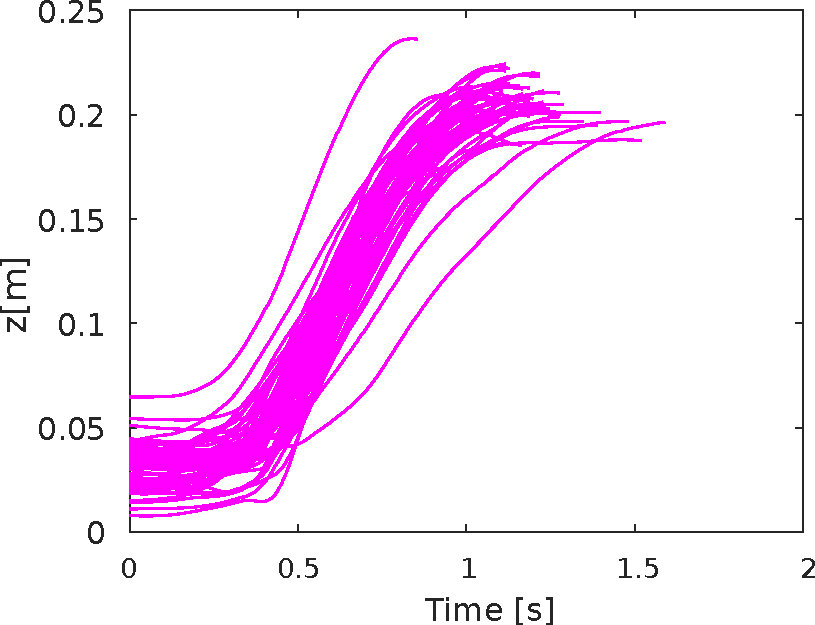
\includegraphics[width=\hsize /2]{img/1DOFtrajectoriesV2.pdf} 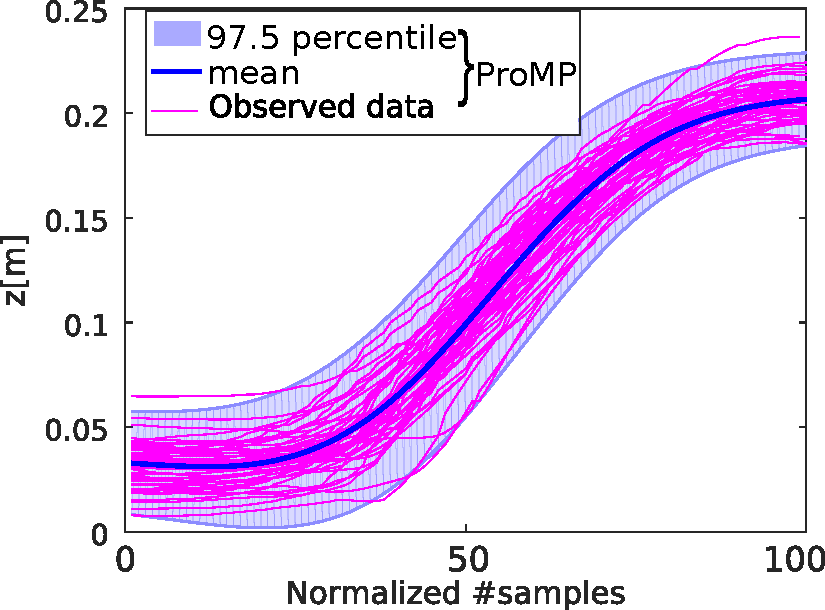
\includegraphics[width=\hsize /2]{img/1DOFtrajectoriesProMPV2.pdf}
%\caption{The trajectories of the test dataset for 1DOF primitive.}
\caption{Les trajectoires observées sont représentées en magenta. La \textit{ProMP} est représentée en bleu. Les paramètres suivants sont utilisés : $\bar{s}=100$ le nombre référence d'échantillons; $M=5$ le nombre de \textit{RBFs} étalées sur la dimension temporelle; et $h=0.04$ (=$ 1 \over M^2$) la variance de ces \textit{RBFs}.}
\label{fig:1DOFtrajectoriesProMP}
\end{figure}

%In this figure, the distribution is represented according to a reference number of samples $\bar{s} = 100$, and the observed trajectory are resaled according to this number of samples, to facilitate the understanding.

Afin de permettre le débogage ainsi que de comprendre comment régler les paramètres des \textit{ProMPs}, il est intéressant de représenter dans un graphique les fonctions à bases radiale en fonction du temps. En effet, choisir le bon nombre de fonctions à bases radiales est important puisque, lorsqu'elles ne sont pas assez, les trajectoires ne peuvent pas être bien approximées et lorsqu'elles sont trop nombreuse, cela peut provoquer des problèmes de surapprentissage. Pour représenter ces fonctions dans u graphique, la fonction suivante peut être appellée : 

\mcode{drawBasisFunction(promp.PHI,M)}

où \mcode{promp.PHI} est un ensemble de \textit{RBFs} évaluées dans la plage temporelle normalisée : $t \in [1:\bar{s}]$.
%, each of which being evaluated at a different time $t \in [1:\bar{s}]$. \todo{is it better?}%during the interval: $\Phi_{[1:\bar{s}]}$ \todo{reformulate this}. 

La Figure~\ref{fig:1DOFtrajectoriesProMPbasis} représente en haut les fonctions à bases radiales avant la normalisation, et en bas la \textit{ProMP} modelé à partir de ces fonctions. De gauche à droit, le nombre de fonctions change. Quand il n'y a pas assez de fonctions (gauche), le model n'es pas capable de représenter correctement la forme des trajectoires. Au milieu, les trajectoires sont correctement représentées par les $5$ fonctions. Avec plus de fonctions (droite), la variance de la distribution décroît parce que le model est plus précis. 
Cependant, augmenter arbitrairement le nombre de fonctions à base radial n'est pas une bonne idée, puisque à un certain moment, ça n'améliore plus la précision du modèle et pire, ça peut provoquer du surapprentissage.
%\rev{With too many basis function, there is no real improvement of the accuracy and it may be overfitting}.
%As a balance, the computation time increases.

\begin{figure}[h]
\centering
{
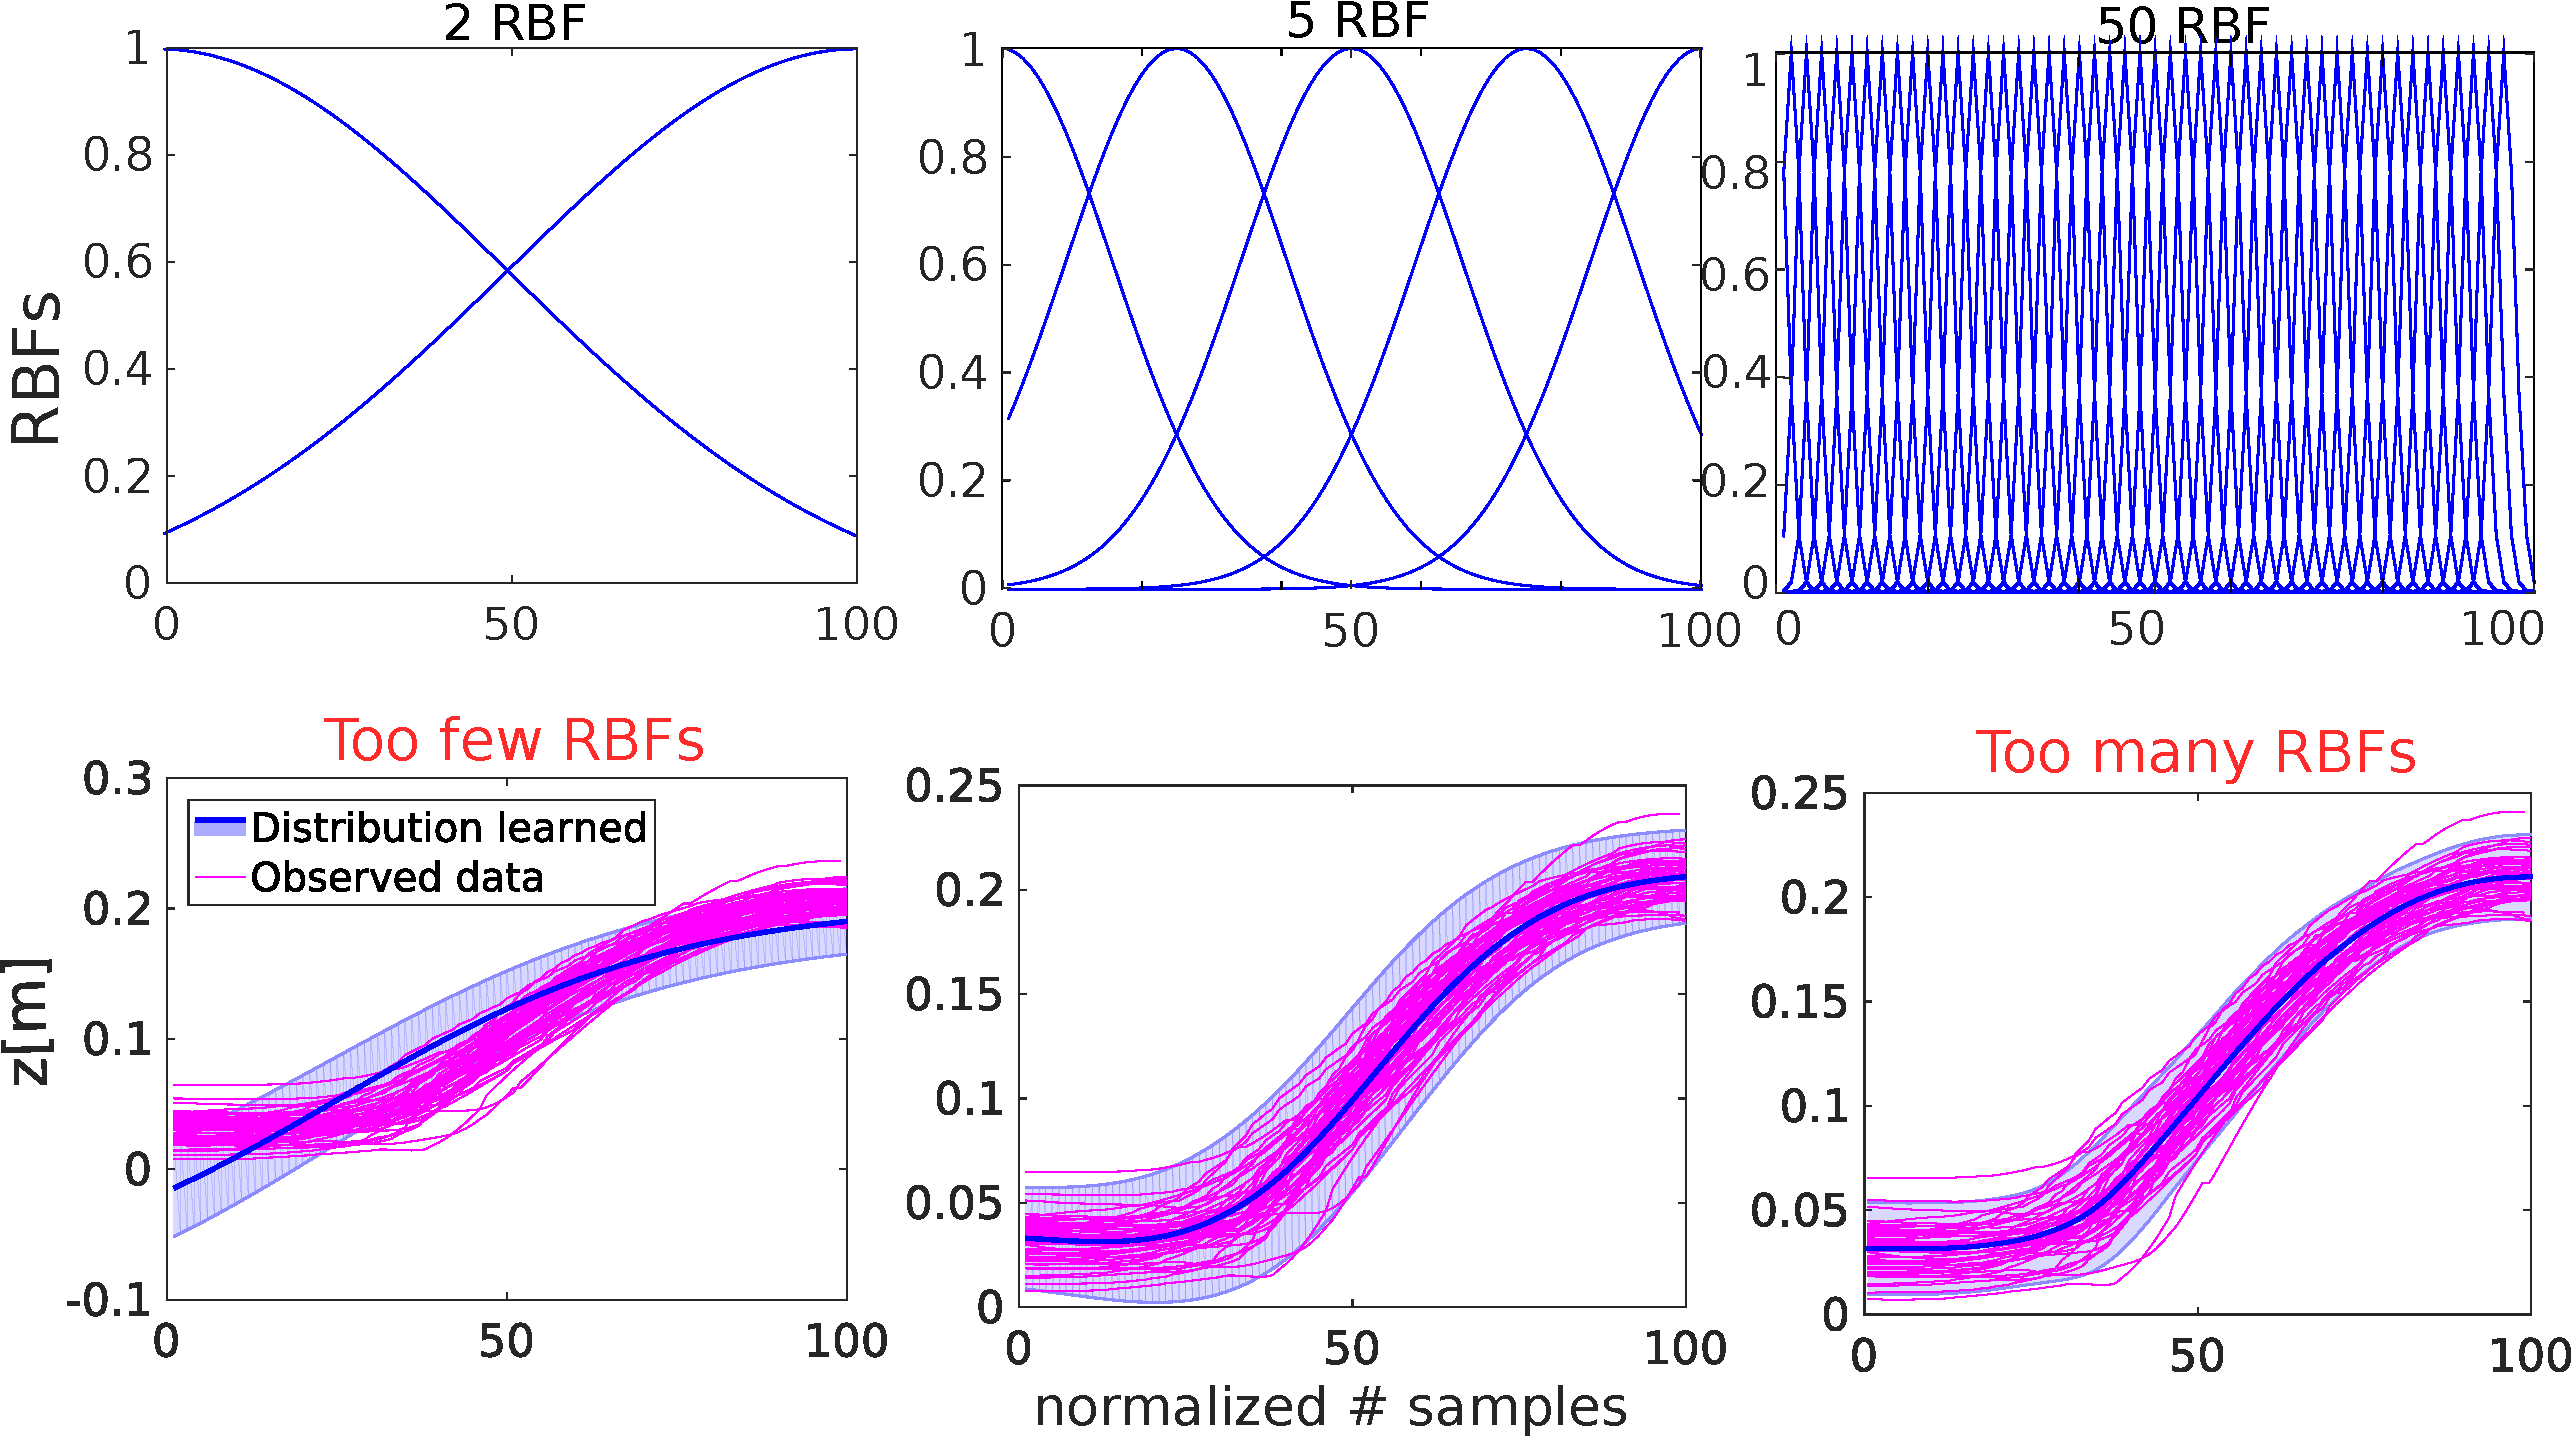
\includegraphics[width=\hsize]{img/1DOFtrajectoriesProMPbasisV4.pdf}
}
\caption{La \textit{ProMP} calculé pour l'ensemble de trajectoire \toimprove{test (?)} (Figure \ref{fig:1DOFtrajectoriesProMP}) en utilisant différents nombres de fonctions à base radiale : de gauche à droite : $M=\{2,5,50\}$ fonctions avant normalisation, de variance $h={1 \over M^2}$. }
\label{fig:1DOFtrajectoriesProMPbasis}
\end{figure}

Après que la \textit{ProMP} soit apprise, le robot est capable de reproduire le mouvement en utilisant la moyenne de la distribution.
De plus, il peut aussi reconnaitre le mouvement qui a été initié dans cette distribution, et prédire comment le finaliser. Dans ce but, à partir de $n_{o}$ observations initiales d'un mouvement, le robot mets à jour la distribution à priori afin qu'elle passe par les mesures observées : en utilisant le conditionnement, il trouve la distribution postérieur, qui peut être utilisée par le robot afin d'executer la continuation du mouvement par lui même.

La première étape pour prédire l'évolution de la trajectoire est d'inférer la durée de cette trajectoire, qui est encodée par le paramètre de modulation du temps $\hat{\alpha}$. Le calcul de cette inférence, qui était détaillé dans la Section~\ref{sec:predictDuration}, peut être effectué à l'aide de la fonction :

\mcode{[expAlpha,type,x]=inferenceAlpha(promp,test\{1\},M,s_ref,c,h,test\{1\}.nbData, expNoise, typeReco)}

où \mcode{typeReco} est le critère utilisé afin d'estimer le paramètre de modulation du temps (\textit{e.g.}, 'MO', 'DI' ou 'ML' pour ``modélisation'', ``distance'' ou ``maximum de vraisemblance''); \mcode{expAlpha} $=\hat{\alpha}$ l'estimation du paramètre de modulation ; \mcode{type} (noté $k$ dans cette thèse) l'index de la \textit{ProMP} à partir de laquelle \mcode{expAlpha} a été calculée. 

%\mcode{x} is used for debugging purpose.
%\marco{Finally \mcode{x = test\{1\} + offset} is the trajectory transposed by an offset, to be centred on the moyenne of the recognized ProMP at time $t=1$ (only used for debugging purposes).[Obs.: I didn’t understand
%584 this.] }
%\rev{it is hard to explain in the paper, but from the early-trajectory, to recognize which ProMPs correspond the best to the initiated trajectory, I need to translate the early-trajectory to compute how likely the "shape" of the early-trajectory correspond to the ProMP}
Afin de prédire l'évolution de la trajectoire, on utilise l'Équation~\ref{eq:inf} de la Section \ref{sec:predict}. Dans Matlab, ce calcul est effectué au sein de la fonction :

\mcode{infTraj = inference(promp, test\{1\}, M, s_ref, c, h, test\{1\}.nbData, expNoise, expAlpha)}\\
où \mcode{test\{1\}.nbData} est calculé durant l'étape \mcode{partitionTrajectory}. Cette variable représente le nombre $n_o$ d'observations, calculée à partir du pourcentage \mcode{percentData} de données de la trajectoire test observées par le robot. \mcode{infTraj}$= \hat{\Xi}$ correspond à la trajectoire prédite.
Finalement, la trajectoire inférée est représentée à l'aide de  la fonction \mcode{drawInference(promp,inputName,infTraj, test{1},s_ref)}.

La qualité de la trajectoire inférée en fonction du nombre d'observations est représentée dans la Figure \ref{fig:1DOFtrajectoriesPredictions}.

\begin{figure}[h]
\centering
{
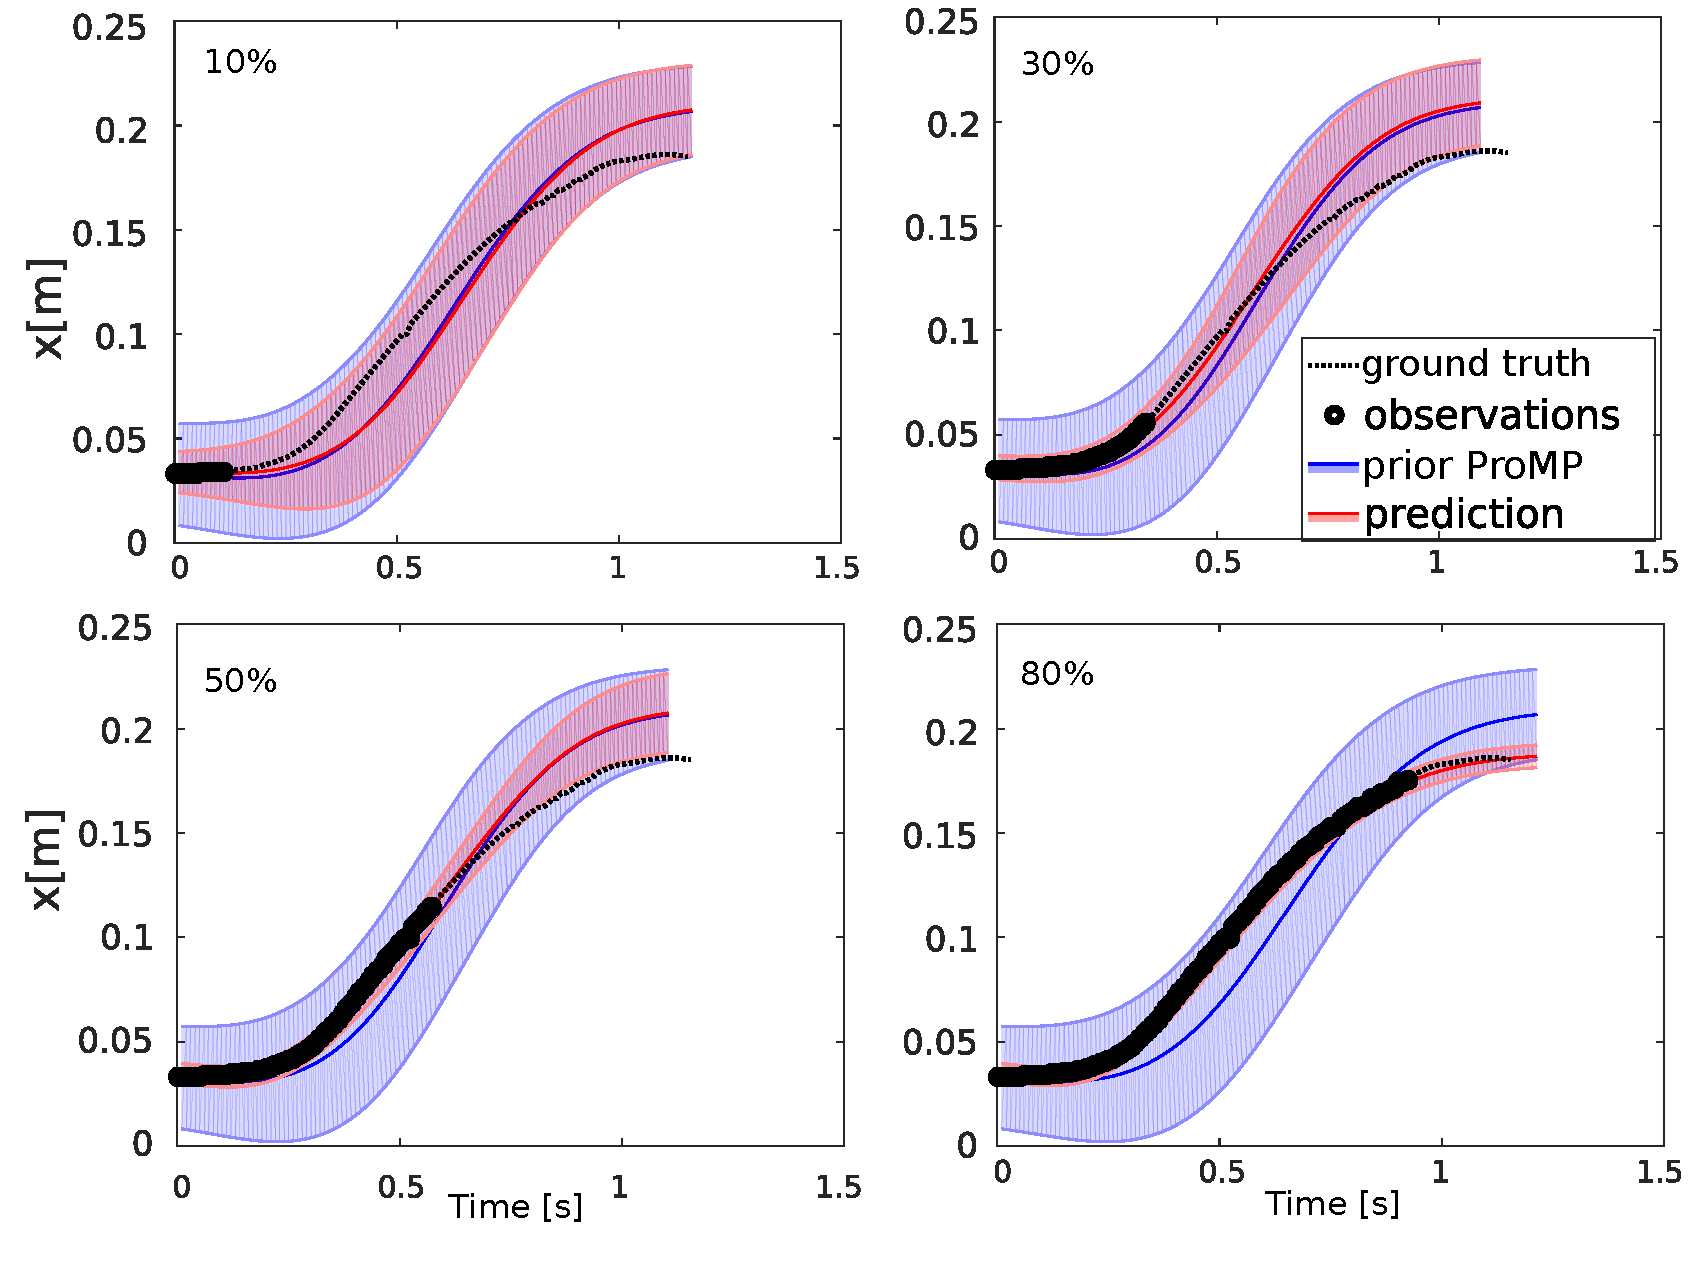
\includegraphics[width=15cm]{img/1DOFtrajectoriesPredictionsV2.pdf}
}
\caption{Prédiction de la continuation de la trajectoire testée, à partir de l'observation des observations partielles et de l'information de la \textit{ProMP} apprise (Figure \ref{fig:1DOFtrajectoriesProMP}). Les graphes représentent la trajectoire prédite après l'observation de 10\%, 30\%, 50\% and 80\% des données de la trajectoire totale.}
% \marco{[This paper explained how to compute the posterior over $\omega$, but not how to
%compute the prior nor the posterior over trajectories. However this must be computed somewhere
%to generate figures such as this one.]} \rev{I don't understand, in eq~\ref{eq:w} we explain how the prior is computed}}
\label{fig:1DOFtrajectoriesPredictions}
\end{figure}

Cette figure met en avant que, lorsqu'une partie importante de la trajectoire est observée, la prédiction de la continuation du mouvement est plus précise.

Après cette étape de prédiction, nous proposons de mesurer la qualité de ces prédictions. Soit $\Xi^* = [\xi^o(1),\ldots, \xi^o({n_o}), \xi^*(n_o+1),\ldots, \xi^*(t^*_f)]$ la trajectoire réelle, espérée par l'utilisateur (ou vérité terrain). 
Afin de mesurer la qualité de la prédiction, plusieurs mesures peuvet être utilisées :
\begin{itemize}
\item La vraisemblance d'avoir une trajectoire $\Xi^*$ sachant la distribution postérieur $p(\boldsymbol{\hat{\omega}})$.
\item La distance entre la trajectoire désirée $\Xi^*$ et la trajectoire inférée $\hat{\Xi}$.
\end{itemize}

Cependant, suivant la mesure \mcode{typeReco} utilisée pour l'estimation du paramètre de modulation du temps $\alpha$ (estimation faite à partir des données initiales observées), un écart visible peut avoir lieu entre la trajectoire prédite et la trajectoire réelle  et ce, même lorsque beaucoup de données sont observées. Cet écart est  provoqué par l'erreur d'estimation du paramètre de modulation du temps. C'est pourquoi, dans la Section \ref{sec:predictDuration}, différentes méthodes seront présentées afin de permettre de prédire la durée de la trajectoire à continuer. Ces méthodes sélectionnent le paramètre $\hat{\alpha}$ le plus probable selon différents critères : distance; maximum de vraisemblance; modélisation de la variable $\alpha$ \footnote{Cette modélisation se base sur l'hypothèse que le paramètre de modulation du temps peut être estimé à partir de la connaissance de la variation \toimprove{``grossière''} de la position lors des $n_o$ premières données observées.}; et la moyenne des paramètres $\alpha$ observés lors de la phase d'apprentissage.
%
%\todo{Je ne pense pas mettre l'exemple ci dessous que tu souhaitais parce que le code est assez long. \\
%In Matlab, this further prediction can be done by:}
%
%\begin{lstlisting}
%for i = 1:3
%	if i >= 5 && a ~= b       % literate programming replacement
%		disp('cool');           % comment 
%	MATLAB CODE
%end
%\end{lstlisting}

La Figure~\ref{fig:1DOFtrajectoriesPredictionsDuration} présente les différentes trajectoires prédites après l'observation de $n_{o}=40\%$ de la trajectoire désirée, en fonction de la méthode utilisée pour estimer le paramètre de modulation du temps. 

Dans ce simple test, où la variation du temps est petite comme présentée dans la Table \ref{tab:alphaProMP}, le meilleur des résultats est accomplis avec la méthode de la moyenne des paramètre de modulation du temps des trajectoires de démonstrations (utilisées lors de la phase d'apprentissage). Dans des cas plus compliqués, lorsque la durée des trajectoires varient plus fortement, les autres méthodes peuvent être préférables, comme présenté dans la Section~\ref{sec:ManyProMP}.
\begin{table}
\center
\begin{tabular}{|p{2.5cm}|p{2.5cm}|p{4.5cm}|p{2.5cm}|}
  \hline
    & \#observations & $\alpha = {\bar{s} \over \mathrm{Iterations}}, \bar{s}=100$ & Durée [s] \\
     \hline
     Minimum & 83 & 1.2048 & 0.83 \\
     \hline
     Maximum & 115 & 0.8696 & 1.15\\
     \hline
     Moyenne & 100& 1& 0.99 \\
     \hline
     écart type & 9 & 11.1111 & 0.09 \\
     \hline
\end{tabular}
\caption{information concernant la durée des trajectoires}
\label{tab:alphaProMP}
\end{table} 

\begin{figure}[h]
\centering
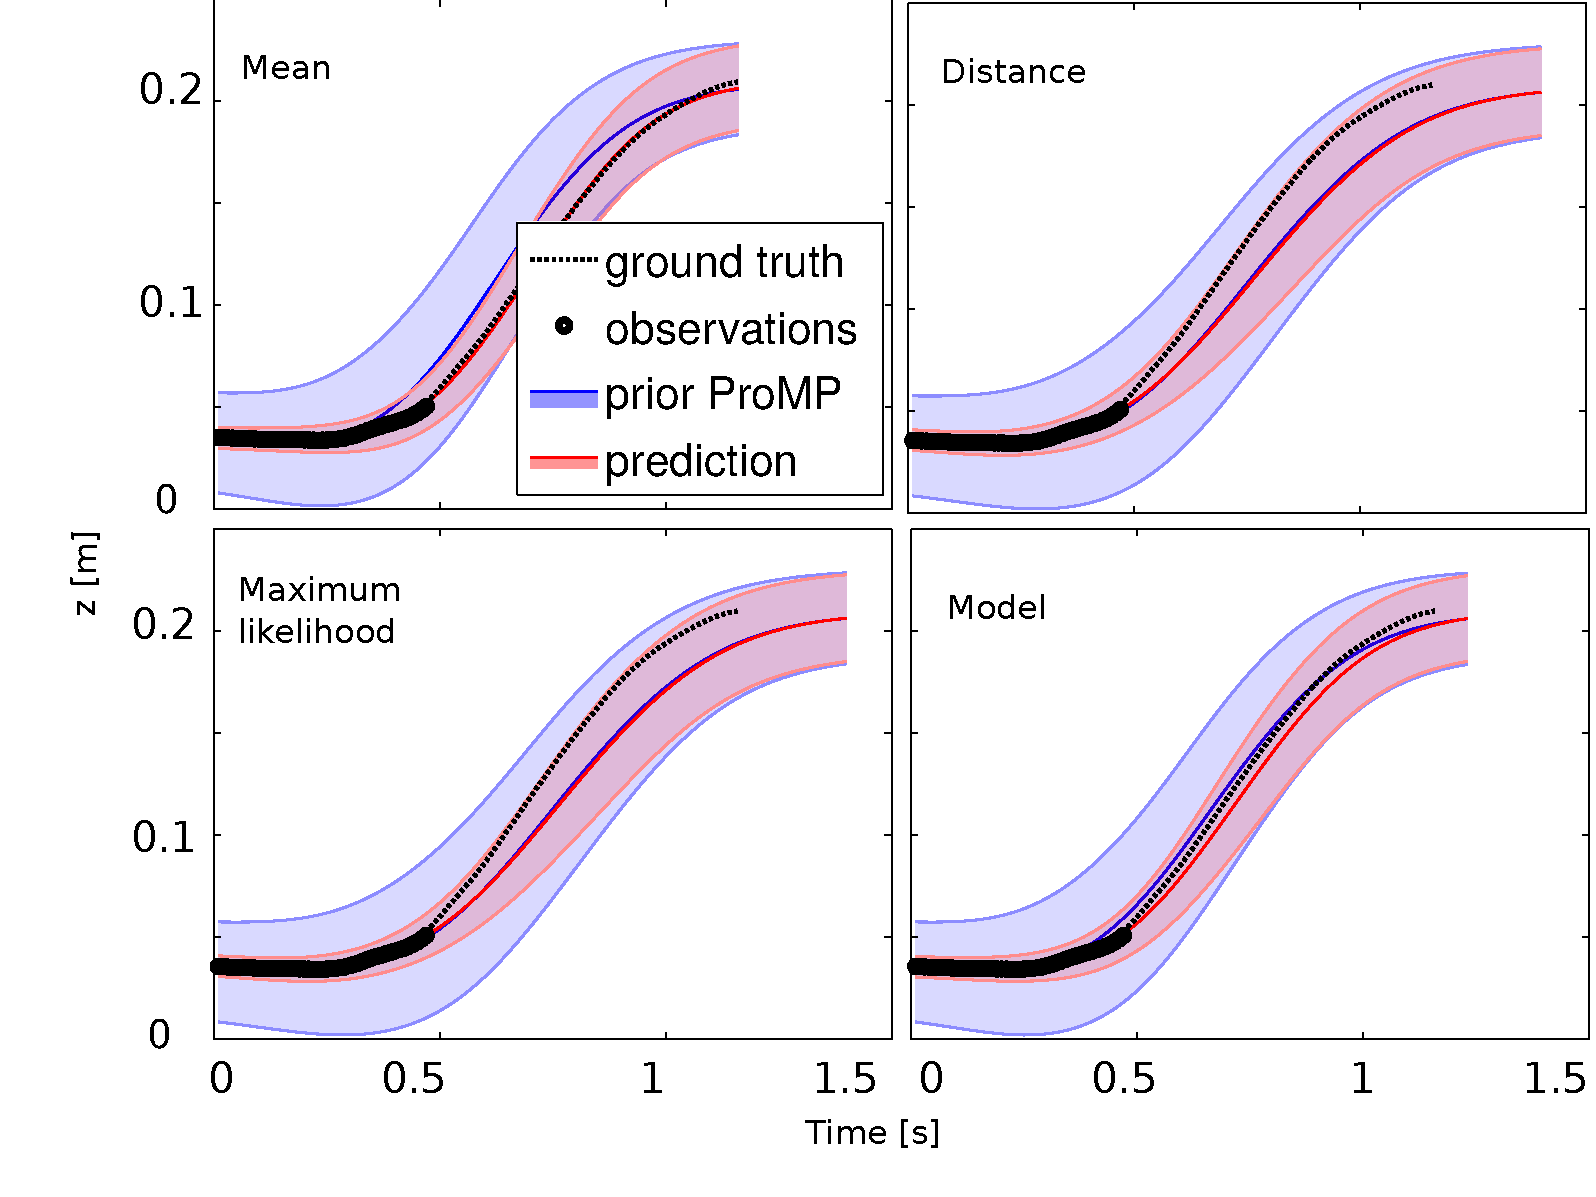
\includegraphics[width=15cm]{img/1DOFtrajectoriesPredictionsDurationV2.pdf}
\caption{Prédiction de la trajectoire future après l'observation de  $n_{o}=40\%$ d'une trajectoire de l'ensemble de test, à l'aide de la \textit{ProMP} apprise (Figure \ref{fig:1DOFtrajectoriesProMP}). Les graphiques représentent la trajectoire prédite en fonction du critère utilisé afin d'estimer le paramètre de modulation du temps qui correspond le plus à la trajectoire initiée : moyenne des paramètre de modulation du temps (Équation~\ref{eq:avg}); distance (Équation~\ref{eq:minDist}); maximum de vraisemblance (Équation~\ref{eq:ml}); ou modélisation de ce paramètre \toimprove{en fonction de la variation temporelle} (Equation~\ref{eq:model}).}
\label{fig:1DOFtrajectoriesPredictionsDuration}
\end{figure}


%%%%%%%%%%%%%%%%%%%%%%%%%%%%%%%%%%%%%%%%%%%%%%%%%%%%%%%%%%%%%%%%%%%%%%%%%%%%%%%%
\section{Application à la simulation du iCub : apprentissage de trois primitives}
\label{sec:3ProMPsAppli}
\begin{figure}[h]
\centering
{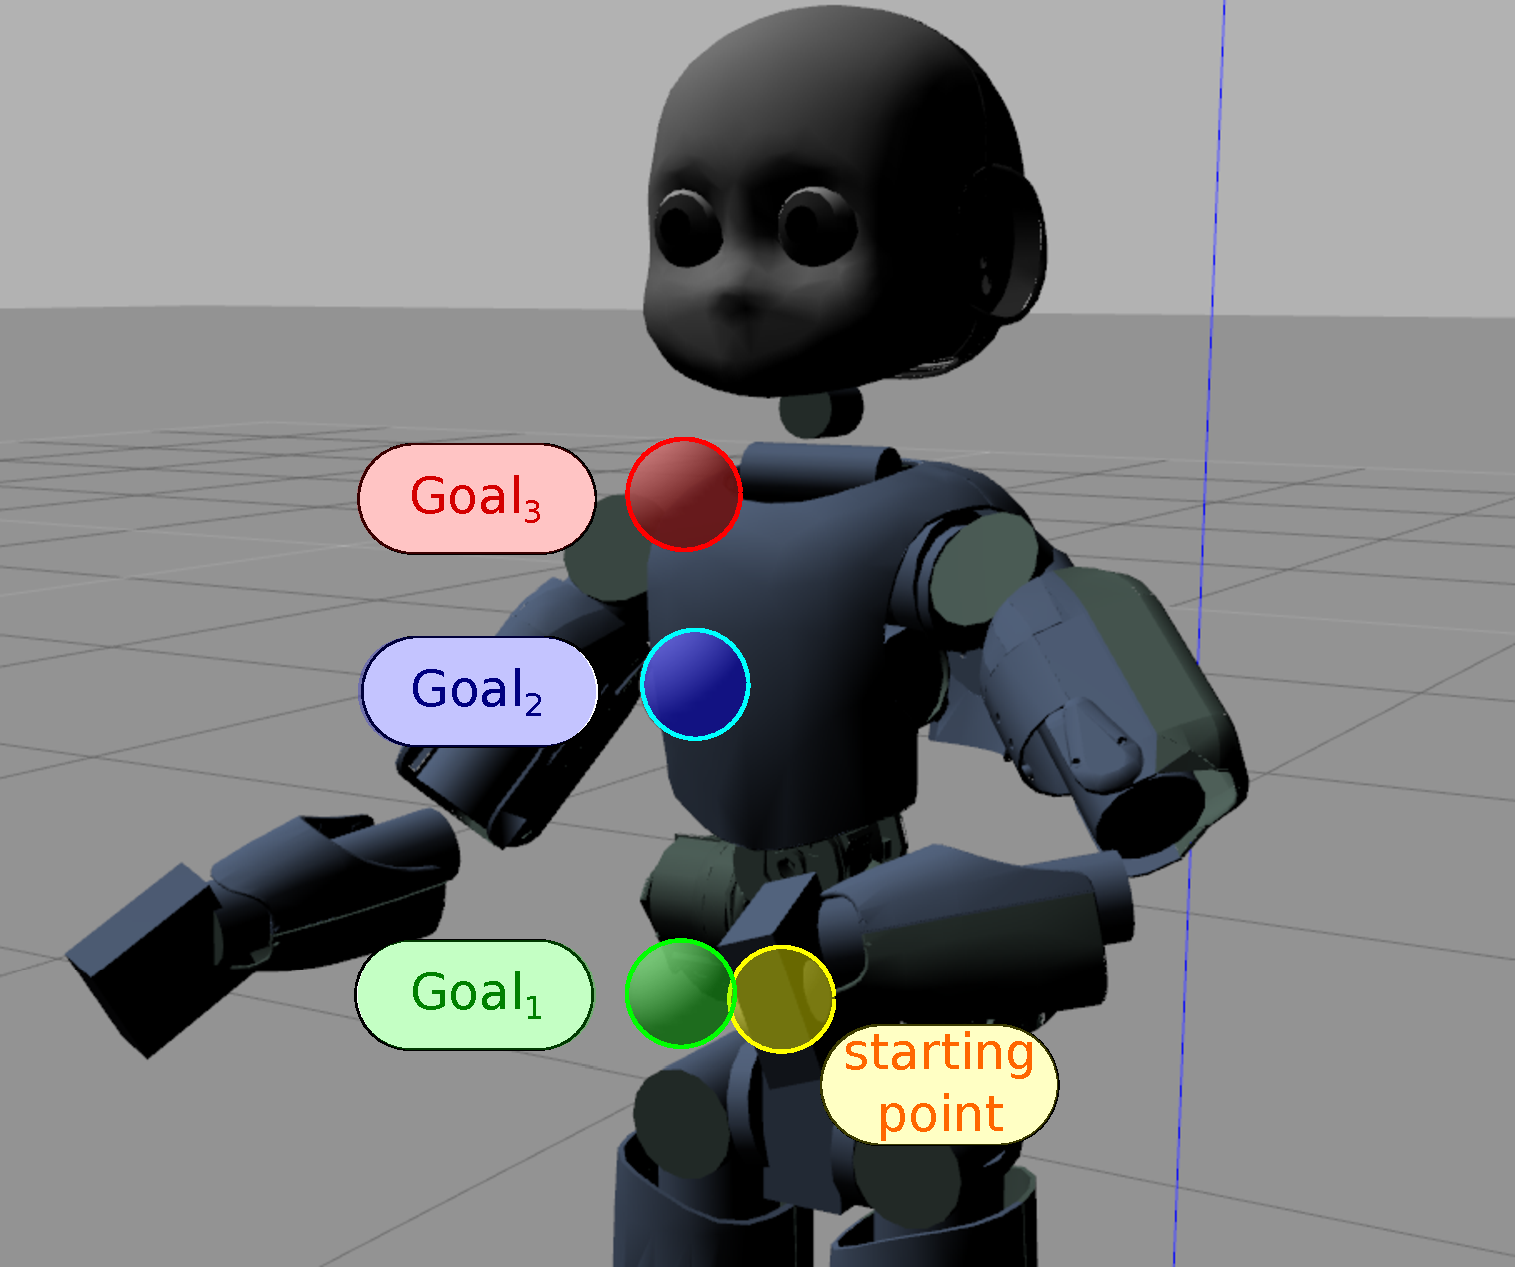
\includegraphics[width=8cm]{img/gazeboGoalsV2.pdf}
\hspace{0.1cm}
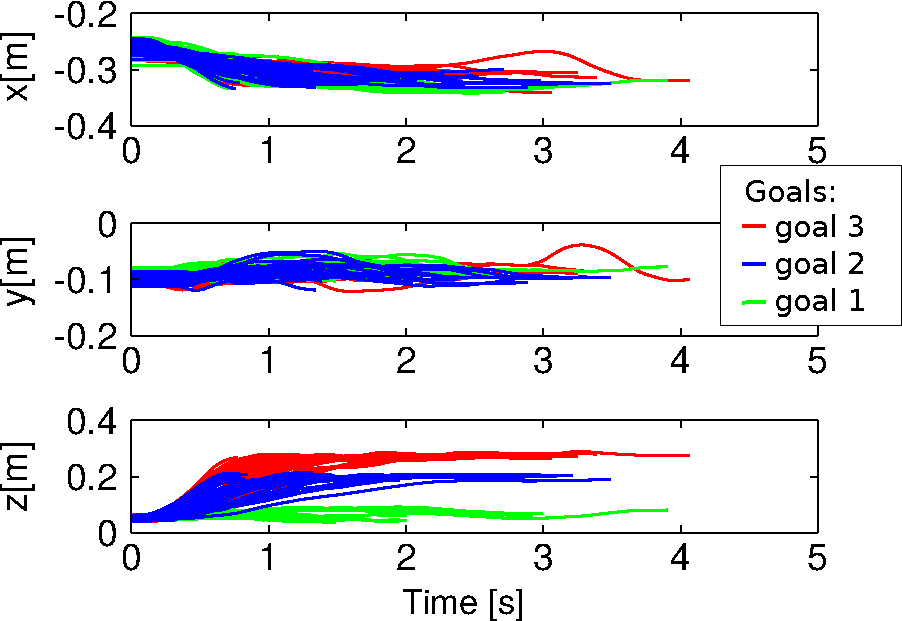
\includegraphics[width=9cm]{img/3DOFtrajectories.pdf}
}
\caption{Gauche : les trois buts colorés que le robot doit atteindre à partir d'un point de départ ; les trajectoires correspondantes sont utilisées afin d'apprendre trois primitives, représentant trois actions. 
Droite: L'information de la position cartésienne des trajectoires de démonstration pour les trois sortes de tâches.}% trajectories x (top),y(middle) and(bottom) without force information that are also recorded.}
\label{fig:3TargetsTrajectories}
\label{fig:GazeboGoal}
\end{figure}

Dans cette application, le robot apprend plusieurs \textit{ProMPs} et est capable de prédire la continuation d'une trajectoire initiée par l'utilisateur, avec l'hypothèse que le mouvement appartienne à l'une des primitives apprises. À partir de cette prédiction, le robot peut aussi finir le mouvement.. 

Les trois actions/tâches sont représenter par les trois buts différents à atteindre, représentés par trois balles colorés et positionnés dans la \toimprove{zone de mouvement} du iCub. L'exemple est effectué à l'aide du robot simulé dans \textit{Gazebo}. La Figure~\ref{fig:GazeboGoal} représente les trois buts, placés à différentes hauteurs, en face du robot.

Dans la Section~\ref{sec:formulateModelInt}, le problème de reconnaissance de l'intention est formulé avec le robot iCub : il s'agit de permettre au robot d'apprendre des \textit{ProMPs} à partir de trajectoires définies par des positions Cartésiennes en 3D\footnote{Remarquons que dans cet exemple spécifique, l'orientation n'est pas utilisée avec le souhait que la main du robot conserve la même orientation durant l'ensemble du mouvement (fixé à priori). Mais en principe, il est possible d'apprendre des trajectoires définis par des positions Cartésiennes et orientation de la main du robot en 6D ou 7D. Ainsi, le robot apprend à changer l'orientation de sa main lors du mouvement.} et l'information des couples en 6D qui sont mesurés par le robot durant l’exécution du mouvement.
Dans la Section \ref{subec:Setup}, la configuration de la simulation du robot iCub dans Gazebo est présentée, puis la Section~\ref{sec:dataAquisition} permet d'expliquer comment les trajectoires sont enregistrées, avec notamment l'information des forces, lors de l'utilisation du robot simulé.


\subsection{Prédire les trajectoires attendues à l'aide de \textit{ProMPs}}\label{sec:formulateModelInt}

Il s'agit d'augmenter la modélisation présentée dans la Section~\ref{sec:theory} afin que la \textit{ProMP} soit composée de plusieurs informations sur la trajectoire. Pour cela, ces informations sont enregistrées dans un vecteur paramètre multivarié :
$$\forall t, \xi_t=\begin{bmatrix} X_t \\ F_t\end{bmatrix} \in \mathbb{R}^{9}$$ 
Où $X_t \in \mathbb{R}^{3}$ correspond à la position cartésienne de l'actuateur du bras de iCub et $F_t \in \mathbb{R}^6$ les forces et moments externes, provenant notamment des forces de contact que l'utilisateur exerce sur le robot. Soit dim($\xi_t$)$ = D = 9$, la dimension de ce vecteur paramètre. %Let $\xi_{inf} =[\xi_{o+1} \ldots \xi_{t_{f}}]^\top$ the output vector of the expected end trajectory, where $t_f$ is the expected total time of the movement.

La \textit{ProMP} est alors représentée par le modèle :
$$\xi_t = \begin{bmatrix} X_t \\ F_t\end{bmatrix} = \Phi_{\alpha t} \boldsymbol{\omega} + \epsilon_t$$
Où $\boldsymbol{\omega} \in  \mathbb{R}^{D \cdot M}$ correspond au vecteur paramètre qui est indépendant du temps ; $\epsilon_t= \begin{bmatrix} \epsilon_{X_t} \\ \epsilon_{F_t}\end{bmatrix} \in \mathbb{R}^D$ correspond au \toimprove{bruit blanc gaussien} \sout{is the zero-moyenne Gaussian i.i.d. observation noise} ; et $\Phi_{\alpha t} \in \mathbb{R}^{D \times D \cdot M}$ est la matrice contenant les \textit{RBFs} \toimprove{à l'itération} $\alpha t$.\\
Puisqu'il s'agit d'un cas multidimensionnel, cette matrice diagonale par bloc $\Phi_{\alpha t}$ est définie par :
$$\Phi_{\alpha t}  = BlockdiagonalMatrix(\phi_1,\ldots,\phi_{D}) \in \mathbb{R}^{D \times D \cdot M} $$
%\left[ \begin{array}{cccc}
% & \hfill & \hfill & \hfill\\
%\hfill & \phi_\xi & \hfill & \hfill\\
%\hfill & \hfill & \ldots &\hfill \\
%\hfill & \hfill & \hfill & \phi_{m_z}
%\end{array} \right] $
Il s'agit d'une matrice diagonale de $D$ \textit{RBFs}, où chaque  \textit{RBF} représente une dimension du vecteur $\xi_t$ et est composée de $M$ fonctions Gaussiennes. Ces $M$ fonctions sont éparpillées dans le temps, afin d'être à valeur sur $[0: \bar{s}]$.


\subsubsection{Apprentissage de Primitives de Mouvement}
\label{learning}
%Assume the robot has to learn $K$ movement primitives.\\

Durant la phase d'apprentissage de chaque primitive de mouvement $k \in [1:3]$, le robot observe différentes trajectoires $S_k = \{\Xi_1,\ldots, \Xi_n\}_k$ (\textit{c.f.} Section~\ref{sec:dataAquisition}).\\
Pour chaque trajectoire $\Xi_{i {[1:t_{fi}]}} = [\xi_{i(1)}, \ldots, \xi_{i(tf_i)}]^\top$, le robot calcule alors le vecteur paramètre optimal $\boldsymbol{\omega}_{ki}$ afin que la modélisation approxime au mieux la trajectoire.

Dans la Section~\ref{sec:ManyProMP}, ces calculs sont présentés. Dans  le logiciel, un calcul matriciel est effectué à la place de $t_{fi}$ calculs itératifs, qui seraient effectués pour chaque observation $t$ (comme dans l'Équation ~\ref{eq:w}). Ainsi, le calcul devient :
\begin{eqnarray}
\boldsymbol{\omega}_{ki} = (\Phi_{\alpha [1:t_{fi}]}^\top \Phi_{\alpha [1:t_{fi}]})^{-1} \Phi_{\alpha [1:t_{fi}]}^\top * \Xi_{i {[1:t_{fi}]}}
\end{eqnarray}
avec $\Phi_{\alpha [1:t_{fi}]} = [\Phi_{\alpha 1}, \Phi_{\alpha 2}\ldots,\Phi_{\alpha t_{fi}}]^\top$.


\subsubsection{Prédiction de l'évolution de la trajectoire à partir d'observations initiales}
\label{prediction}

Après avoir appris les trois \textit{ProMPs}, le robot est capable de finir le mouvement initié par lui même. Les Sections~\ref{sec:predict}, \ref{sec:predictDuration} et \ref{sec:ManyProMP}, présentent les différents calculs permettant d'estimer la trajectoire désirée à partir des observations initiales . %the end of this movement is computed.

Dans cet exemple des spécificités sont ajoutées sur les paramètres à apprendre.

Soit $\Xi^{o} = \begin{bmatrix} X^o \\ F^o \end{bmatrix} = [\Xi_1 \ldots \Xi_{n_o}]^\top$ les premières observations de la trajectoire initiée.

En premier lieu, seule une sous partie de ses observations est considérée : $X^{o} = [X_1 \ldots X_{n_o}]^\top$. Cela se base sur l'hypothèse que la reconnaissance de la trajectoire se fait uniquement avec l'information de sa position Cartésienne, puisqu'une même trajectoire peut être effectuée et reconnaissable quelque soit son profil de forces .
À partir de l'observation partielle de la trajectoire $X^o$, le robot reconnait la \textit{ProMP} courante $\hat{k} \in [1:3]$ (\textit{c.f.} Section~\ref{sec:ManyProMP}). De plus, il calcul une estimation du paramètre de modulation du temps $\hat{t}_f$ (\textit{c.f.} Section \ref{sec:predictDuration}). À l'aide de cette estimation, il approxime alors la vitesse de la trajctoire et sa durée totale.
%\marco{is this expectation in sense of expected value?}
%\rev{yes}

En second lieu, l'ensemble des observations initiales $\Xi^o$ est utilisé afin de mettre à jour la \textit{ProMP} reconnue (\textit{c.f.} Section \ref{sec:predict}). Pour ce faire, un calcul matriciel est effectué, basé sur l'Équation~\ref{eq:udateWithAlpha} :
$$\left\{
\begin{array}{rl}
\hat{\mu}_{\boldsymbol{\omega}_k} &= \mu_{\boldsymbol{\omega}_k}  + K(\Xi^o - \Phi_{\alpha[1:n_o]} \mu_{\boldsymbol{\omega}_k} ) \\ 
\hat{\Sigma}_{\boldsymbol{\omega}_k}  &= \Sigma_{\boldsymbol{\omega}_k}  - K(\Phi_{\alpha[1:n_o]}\Sigma_{\boldsymbol{\omega}_k} ) \\
K&= \Sigma_{\boldsymbol{\omega}_k} \Phi_{\alpha[1:n_o]}^\top(\Sigma_{\xi^o} + \Phi_{\alpha[1:n_o]}\Sigma_{\boldsymbol{\omega}_k}  \Phi_{\alpha[1:n_o]}^\top)^{-1}
\end{array}
\right.$$

À partir de cette distribution postérieure, la trajectoire inférée $\hat{\Xi} = \{ \hat{\xi}_1,..., \hat{\xi}_{\hat{t}_f}\}$ est récupérée par :
$$ \forall t \in [1:\hat{t}_f],\hat{\xi}_t = \begin{bmatrix} \hat{X}_t \\ \hat{F}_t\end{bmatrix} =  \Phi_{\alpha t} \hat{\mu}_{\boldsymbol{\omega}_k} $$
%Using the partial inferred trajectory $\hat{X}$, the robot is able to finish the movement. Using the partial inferred trajectory $\hat{F}$, the robot stays alert to its user's wishes, as presented in Section~\ref{subsec:forces}.

Notons que les forces inférées $\hat{F}_t$ correspondent à des \toimprove{forces} \comment{wrench} simulées dans Gazebo. Dans cet exemple, l'information ds forces est très peu utilisée. L'intérêt de prédire aussi les \toimprove{forces} \comment{wrenches} sera plus claire dans la Section~\ref{sec:appliRealIcub}, lors de l'exemple sur le robot réel.


\subsection{Configurations pour le robot simulé}
\label{subec:Setup}
Pour cette application, nous avons crée un prototype sur Gazebo, où le robot doit atteindre trois différentes positions but, avec l'aide de l'utilisateur. Afin que celui-ci puisse interagir physiquement avec le robot simulé, un dispositif haptique nommé \textit{Geomagic touch} est utilisé.

La configuration consiste en :
\begin{itemize}
\item un robot iCub simulé dans \textit{Gazebo}, comprenant l'information de la dynamique du robot fournie par l'application \textit{wholeBodyDynamicsTree} (\url{https://github.com/robotology/codyco-modules/tree/master/src/modules/wholeBodyDynamicsTree}) et l'information sur les positions cartésiennes du robot fournie par l'application \textit{iKinCartesianController} ;
\item le \textit{Geomagic Touch} qui doit être installé suivant les instructions fournies dans \url{https://github.com/inria-larsen/icub-manual/wiki/Installation-with-the-Geomagic-Touch}, qui installe non seulement le kit de développement et les drivers de ce dispositif, mais aussi informe comment installer les drivers sur \textit{YARP}\todo{expliquer ce que c'est en amont} ;
\item un module C++ (\url{https://github.com/inria-larsen/icubLearningTrajectories/tree/master/CppProgram}) qui renvoi les commandes provenant du Geomagic au iCub simulé et qui permet d'enregistrer des trajectoires fais par le robot simulé dans un fichier. Un tutoriel permettant de comprendre comment utiliser ce module est fourni avec le logiciel.
\end{itemize}

Les connexions entres les différents modules sont représentées dans la Figure~\ref{fig:orgaSoftware}, \toimprove{où le module Matlab n'est pas utilisé} \todo{???}.
%sketched in Figure~\ref{fig:systemHaptic}.
La pointe du stylo du Geomagic est virtuellement attaché à la main du robot :
$$ x_{geo} \rightarrow x_{icub\_hand} $$
Quand l'opérateur bouge le Geomagic, le position de la pointe du stylo du Geomagic $x_{geo}$ est redimensionnée \todo{(1:1 par défaut) ??} dans l'environnement du iCub simulé en tant que $x_{icub\_hand}$ et le contrôleur cartésien du robot est utilisé afin de déplacer la main du robot par rapport soit à une position de départ fixé dans la simulation (l'utilisateur doit alors positionner le Geomagic afin d'atteindre cette position), soit à la position prise au départ par l'utilisateur lorsqu'il appuie sur l'un des boutons du Geomagic :
$$ x_{icub\_hand} = hapticDriverMapping(x_0 + x_{geo})$$
où \textit{hapticDriverMapping} correspond à la transformation appliquée par le dispositif haptique, \toimprove{qui mappe la fenêtre de référence du Geomagic à la fenêtre de référence du iCub.}
Par défaut, dans cette application, aucune force n'est renvoyée à l'opérateur, puisqu'il s'agit de simuler le mode de contrôle à couple nulle du iCub réel (il s'agit d'un mode de contrôle où le robot n'oppose aucune force de résistance, permettant à l'humaine de le guider). Une orientation par défaut est définie dans cette application.

%\begin{figure}[h]
%\centering
%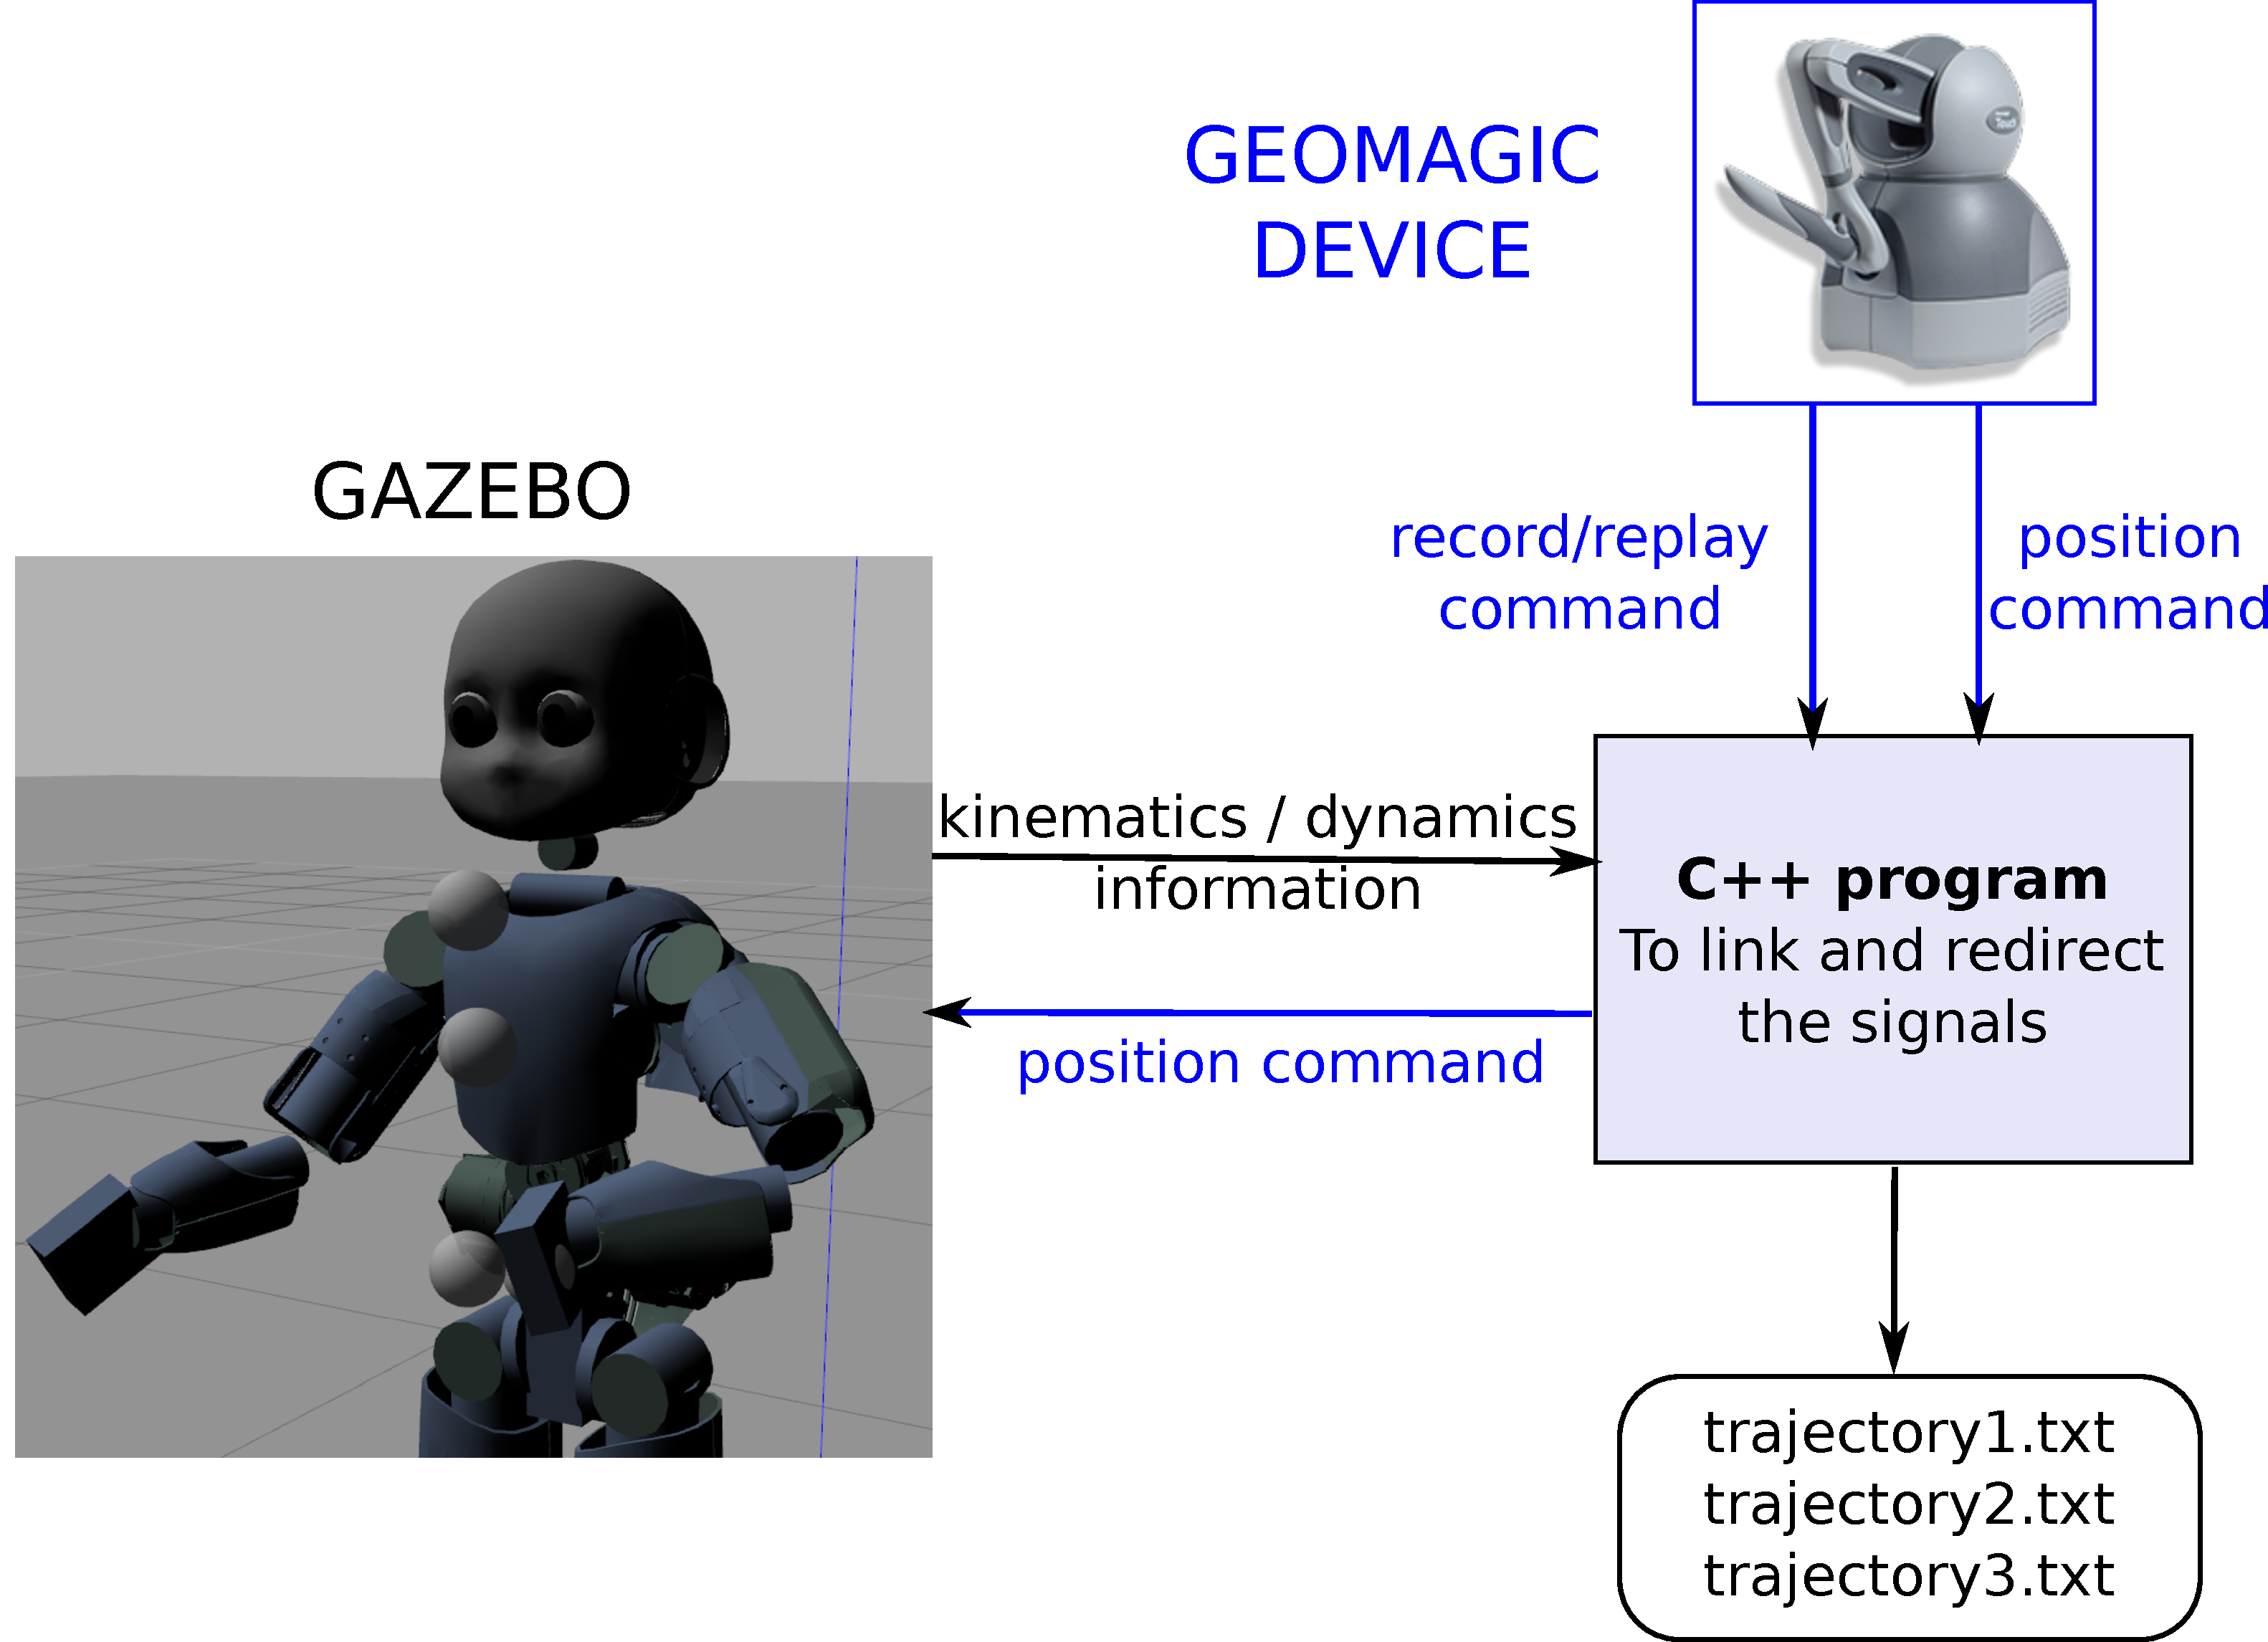
\includegraphics[width=15cm]{img/geom_ctrlV2.pdf}
%\caption{The interconnection between the Geomagic Touch and iCub in Gazebo.}
%\label{fig:systemHaptic}
%\end{figure}

\subsection{Acquisitiom de données}
\label{sec:dataAquisition}
Le bouton sombre du Geomagic est utilisée afin de commencer et d'arrêter l'enregistrement de chaque trajectoire. L'opérateur doit alors cliquer et maintenir ce bouton durant tout son mouvement, puis relâcher celui-ci à la fin de la trajectoire. La trajectoire est sauvegardé dans un fichier nommé \textit{recordX.txt} pour la $X^e$ trajectoire. La structure de ce fichier est :
\begin{lstlisting}
#time #xgeo #ygeo #zgeo #fx #fy #fz #mx #my #mz #x_icub_hand #y_icub_hand #z_icub_hand
5.96046e-06 -0.0510954 -0.0127809 -0.0522504 0.284382 -0.0659538 -0.0239582 -0.0162418 -0.0290078 -0.0607215 -0.248905 -0.0872191 0.0477496$
 \end{lstlisting}
%To replay one of the trajectories from the $N$ previously recorded, the operator can click the light grey button of the Geomagic and then enter the number of the trajectory on the terminal.

%\begin{figure}[h]
%\centering
%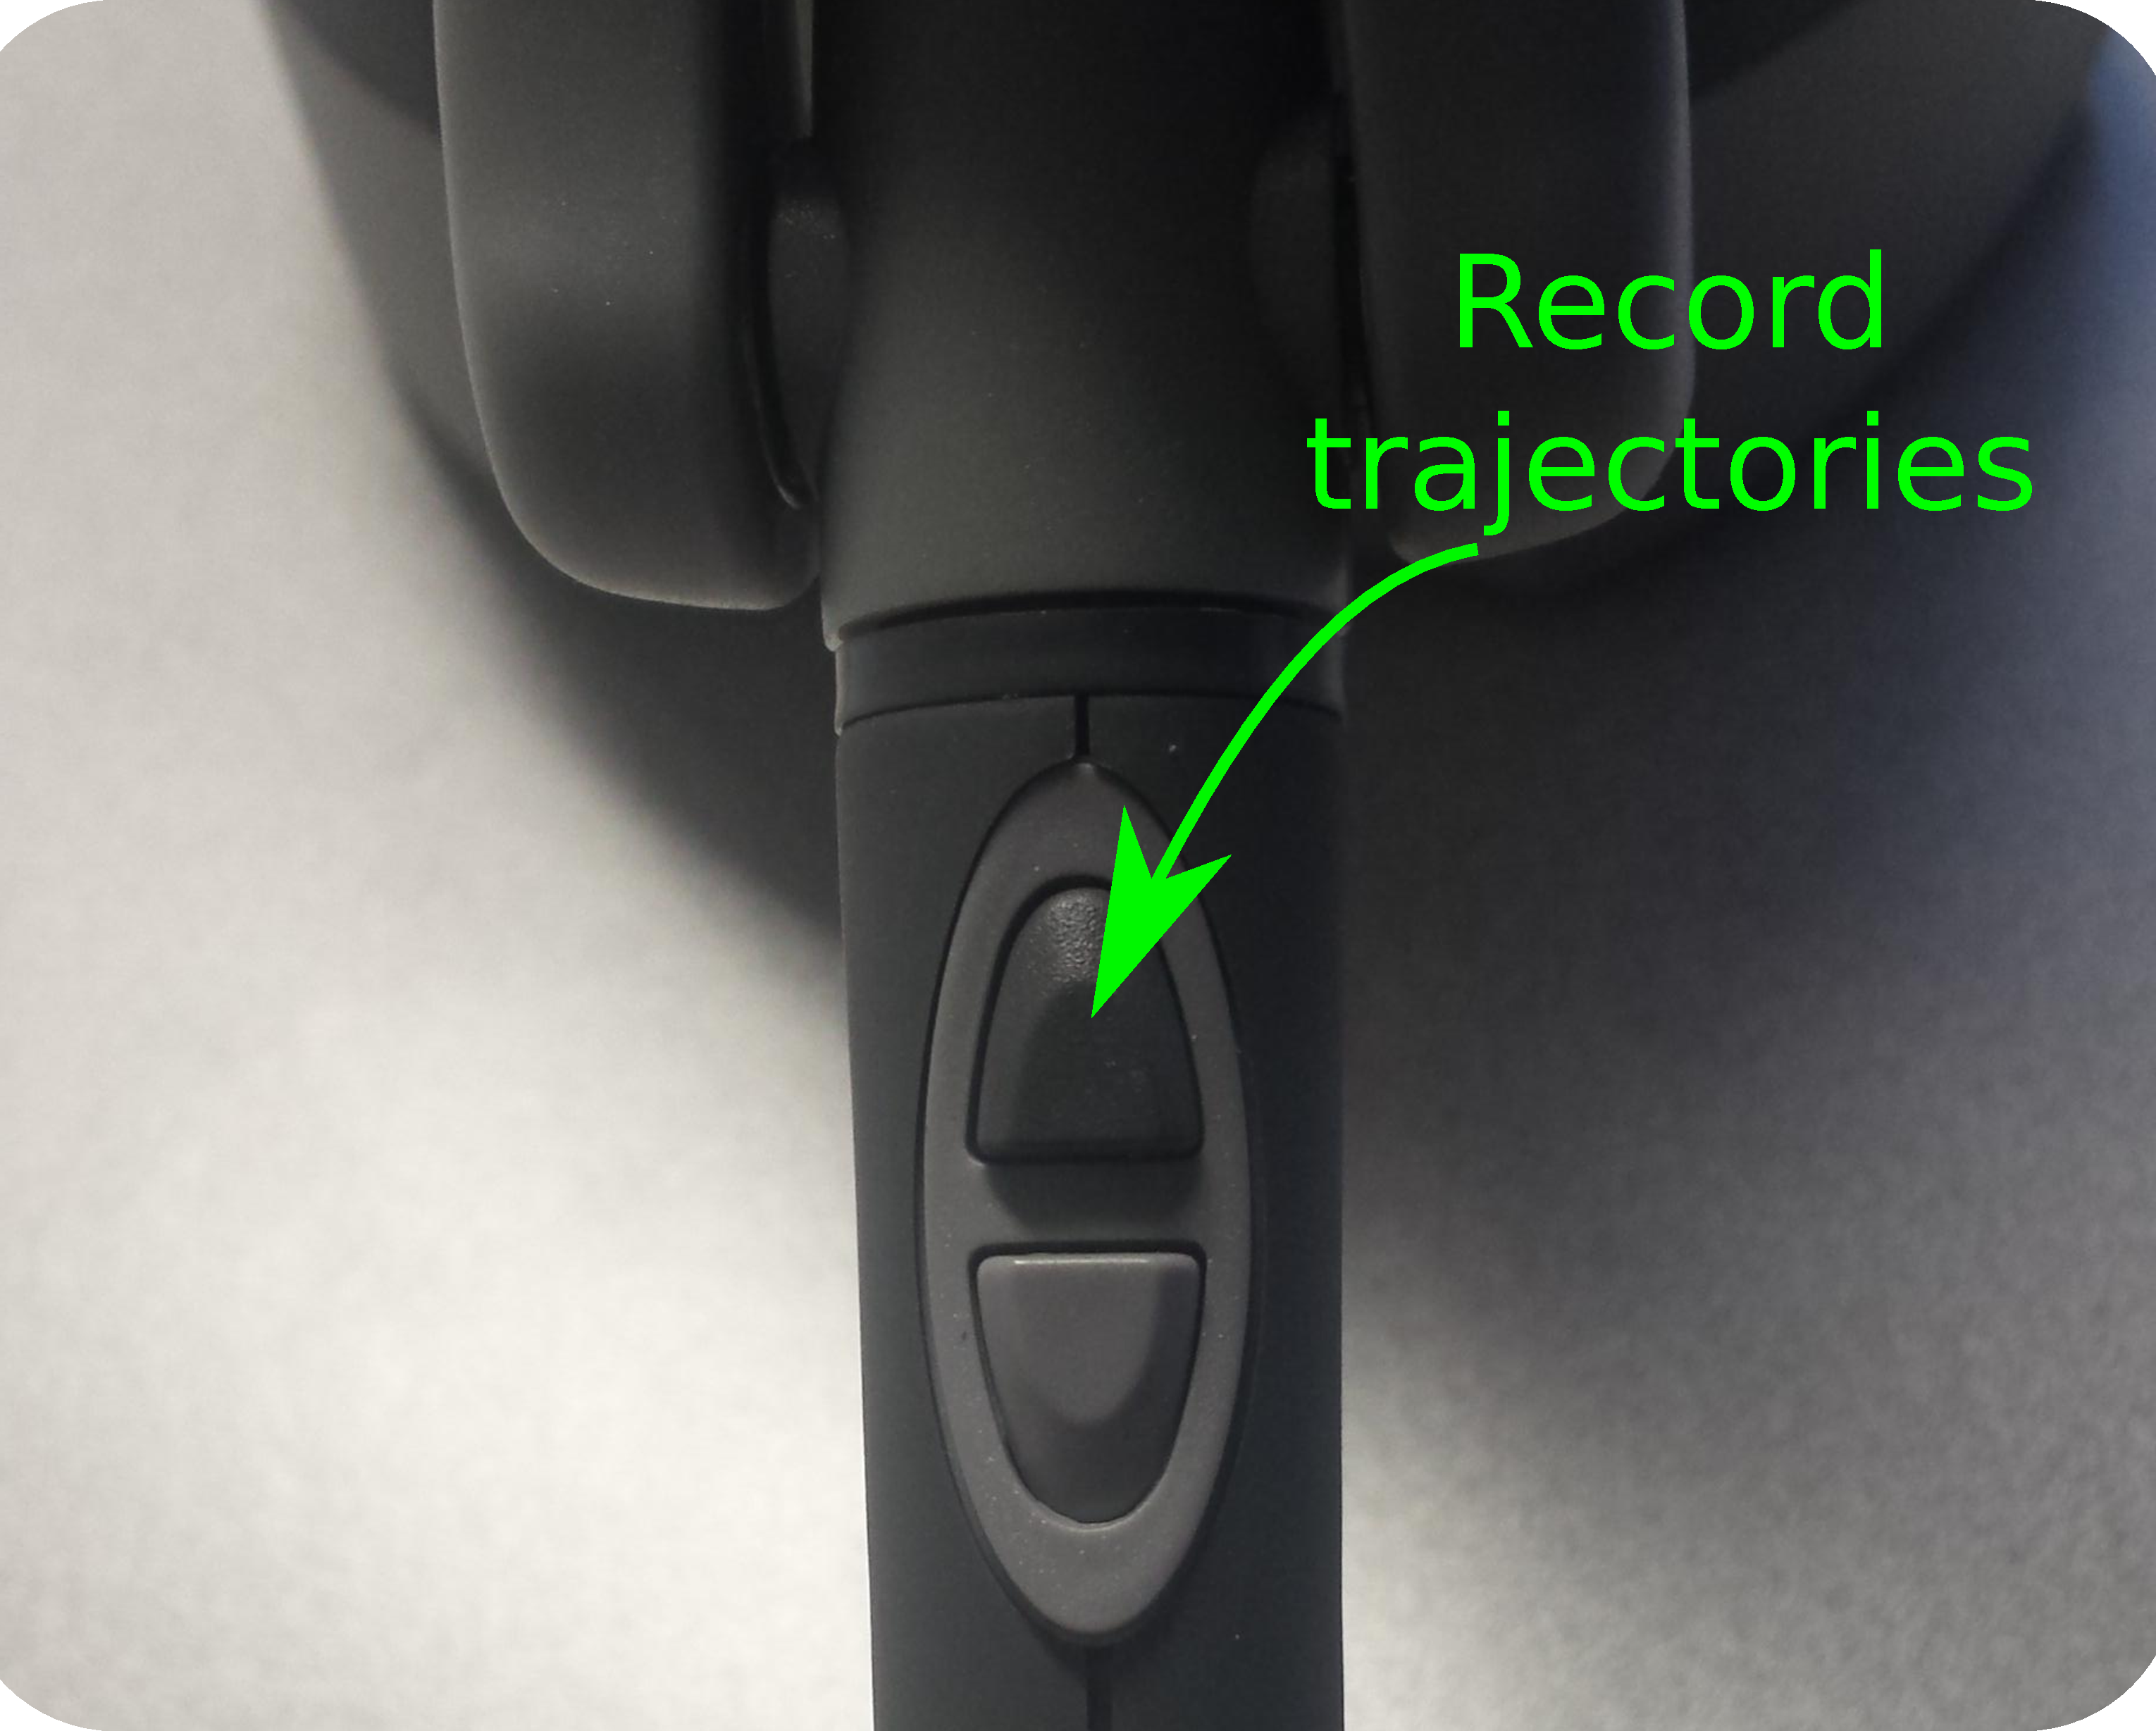
\includegraphics[height = 5cm]{img/geoButton.pdf}
%\caption{The dark button of the Geomagic.}
%\label{fig:geobuttons}
%\end{figure}

Une vidéo représentant cette manipulation, où l'opérateur guide le bras du iCub simulé à l'aide du dispositif haptique est disponible (\textit{c.f.} Section~\ref{sec:video}).
Le graphe de la Figure~\ref{fig:3TargetsTrajectories} représente quelques trajectoires enregistrées à l'aide du Geomagic, lors de la levée du bras gauche du robot \textit{iCub}.

%\begin{figure}[h]
%\centering
%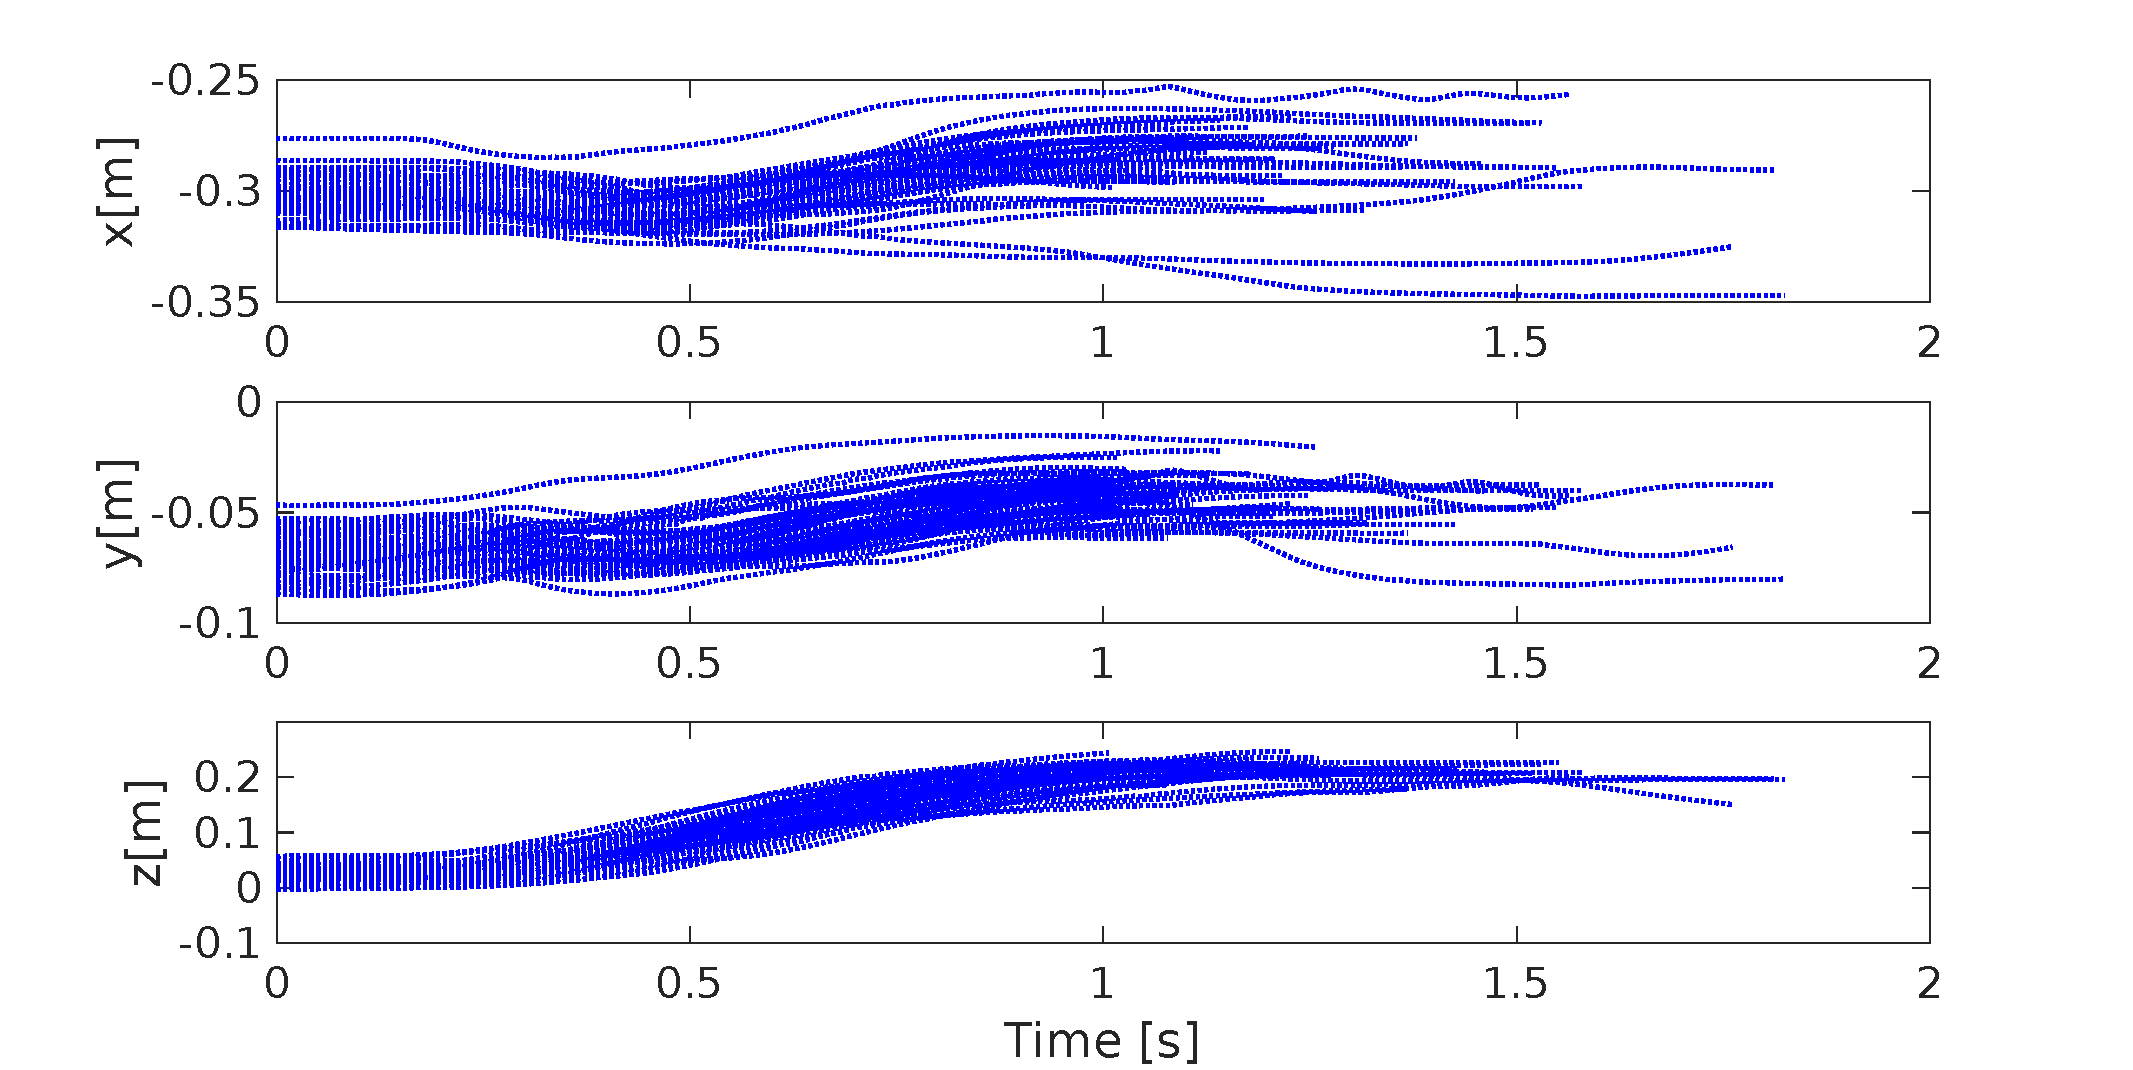
\includegraphics[width=\hsize]{img/liftingWgeomagic/trajectory_sample.pdf}
%\caption{Some trajectories recorded when the Geomagic is used to lift the left arm: Cartesian position of the end-effector.}
%\label{fig:trajectories}
%\end{figure}

Les trajectoires de démonstrations et leurs forces correspondantes peuvent être enregistrées directement, en accédant à l'interface Cartésienne du robot et au module \textit{wholeBodyDynamicsTree}.\footnote{Dans notre exemple, l'information des forces et des couples ne sont pas utilisées car elles sont trop bruitées. Cependant, nous fournissons le code permettant de montrer comment les récupérer et comment les utiliser à partir du Geomagic.}

Dans notre projet Github, nous fournissons l'ensemble des données des trajectoires que nous avons enregistré, pour les utilisateurs qui souhaitent tester le code avec ces trajectoires. Deux ensembles de données sont disponibles à l'adresse \url{https://github.com/inria-larsen/icubLearningTrajectories/tree/master/MatlabProgram/Data/}:  le premier, appelé ``heights", est composé de trajectoires utilisées afin d'atteindre trois positions buts, dont la hauteur varie ; le second, appelé `FLT", est composé de trajectoires effectuées par le vrai robot, et permettent d'atteindre trois type de but : un but positioné devant le robot, un autre sur sa gauche et le dernier en hauteur.

Un script Matlab permet d'apprendre les \textit{ProMPs} à partir d'ensemble de trajectoires enregistrées comme celles présentées ci-dessus. Il s'agit du script \mcode{demo_plotProMPs.m} qui contient les étapes présentées ci-dessous.

Afin de récupérer l'ensemble de données ``\textit{heights}", le script suivant est appelé :
\begin{lstlisting}
t{1} = loadTrajectory('Data/heights/bottom', 'bottom', 'refNb', s_bar, 'nbInput',nbInput, 'Specific', 'FromGeom');
t{2} = loadTrajectory('Data/heights/top', 'top', 'refNb', s_bar, 'nbInput',nbInput, 'Specific', 'FromGeom');
t{3} = loadTrajectory('Data/heights/middle', 'forward', 'refNb', s_bar, 'nbInput',nbInput, 'Specific', 'FromGeom');
\end{lstlisting}

La Figure \ref{fig:3TargetsTrajectories} représente ces trois groupes de trajectoires de démonstration contenu dans l'ensemble ``\textit{height}''. Dans cet ensemble, $40$ trajectoires ont été enregistrées par primitive de mouvement.

%\begin{figure}[h]
%\centering
%{
%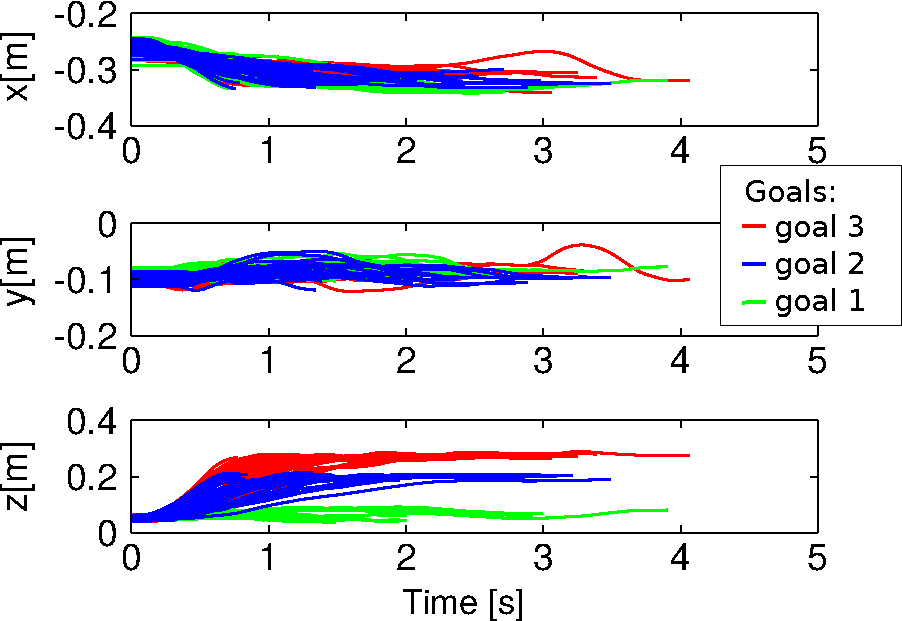
\includegraphics[width=12cm]{img/3DOFtrajectories.pdf}
%}
%\caption{Trajectories guided by the iCub's partner where he reaches three different positions that variate in height: in green the "bottom", in blue "middle" and in red "top goal positions. This plot represents only Cartesian position without force information.}% trajectories x (top),y(middle) and(bottom) without force information that are also recorded.}
%\label{fig:3TargetsTrajectories}
%\end{figure}

\subsection{Apprentissage de \textit{ProMPs}}

Tout d'abord, les \textit{ProMPs} qui correspondent aux trois mouvements observés doivent être apprises. Pour cela, l'ensemble de données est d'abord séparé en deux, la première partie afin d'apprendre les \textit{ProMPs} et la seconde afin de vérifier que la prédiction se fait correctement (trajectoires tests). 
Pour ne conserver qu'une trajectoire test sélectionnée de manière aléatoire, la fonction suivante est appelée:
%Before learning them, we pick from the training set one of the observed trajectory to test the inference, by writing for each $i$-th ProMP:
\begin{lstlisting}
[train{i},test{i}] = partitionTrajectory(t{i},1,percentData,s_bar);
\end{lstlisting}
Le second paramètre d'entrée spécifie qu'une seule trajectoire doit être sélectionnée de manière aléatoire afin de tester la \textit{ProMP} apprise. %With another number, for instance $10$, $10\%$ of the recorded data would be used for tests.
Maintenant, les trois \textit{ProMPs} sont apprises avec :

\begin{lstlisting}
promp{1} = computeDistribution(train{1}, M, s_bar,c,h);
promp{2} = computeDistribution(train{2}, M, s_bar,c,h);
promp{3} = computeDistribution(train{3}, M, s_bar,c,h)
\end{lstlisting}

avec comme paramètres :
\begin{itemize}
\item \mcode{s\_bar=100} : le nombre d'échantillon de référence, noté $\bar{s}$ dans cette thèse.
\item \mcode{nbInput(1) = 3; nbInput(2) = 6} : la dimension du vecteur paramètre qui contien les états de la trajectoire. Il est composé de la position Cartésienne en $3D$ et des forces et couples en $6D$.\comment{\footnote{Note that in our example wrenches are separated from the Cartesian position, because they are not used to recognize the index of the current ProMP during the inference.}}
%\rev{dimension of the generic vector containing the state of the trajectories. It is composed of 3D Cartesian position and 6D forces and wrench information. Wrenches are separated from the Cartesian position, because they are not used to recognize the index of the current ProMP during the inference.}
\item \mcode{M(1) = 5; M(2)= 5}: le nombre de \textit{RBFs} utilisé pour représenter chacune des \mcode{nbInput} dimensions.
\item \mcode{c = 1/M;h = 1/(M*M)}: Les paramètres des \textit{RBF} (\textit{c.f.} Équation~\ref{eq:RBF}).
\item \mcode{expNoise = 0.00001} : le bruit supposé des données.
\item \mcode{percentData = 40} : cette variable spécifie le pourcentage de données de la trajectoire totale que le robot doit mesurer avant de prédire la continuation de la trajectoire.
\end{itemize}

Ces paramètres peuvent être adaptés et sont fixés au début du script Matlab.


La Figure \ref{fig:3TargetsZTrajectoriesProMP} présente les trois \textit{ProMPs} permettant d'atteindre trois positions but répartie à différentes hauteurs. Afin de clarifier ce graphique, seul l'axe $z$ de la position Cartésienne est présenté.

\begin{lstlisting}
drawRecoverData(t{1}, inputName, 'Specolor','b','namFig', 1);
drawRecoverData(t{1}, inputName, 'Interval', [4 7 5 8 6 9], 'Specolor','b','namFig',2);
drawRecoverData(t{2}, inputName, 'Specolor','r','namFig',1);
drawRecoverData(t{2}, inputName, 'Interval', [4 7 5 8 6 9], 'Specolor','r','namFig',2);
drawRecoverData(t{3}, inputName, 'Specolor','g','namFig',1);
drawRecoverData(t{3}, inputName, 'Interval', [4 7 5 8 6 9], 'Specolor','g','namFig',2);
\end{lstlisting}

%We used the following parameters \todo{explain params...}

%\begin{figure}[h]
%\centering
%{
%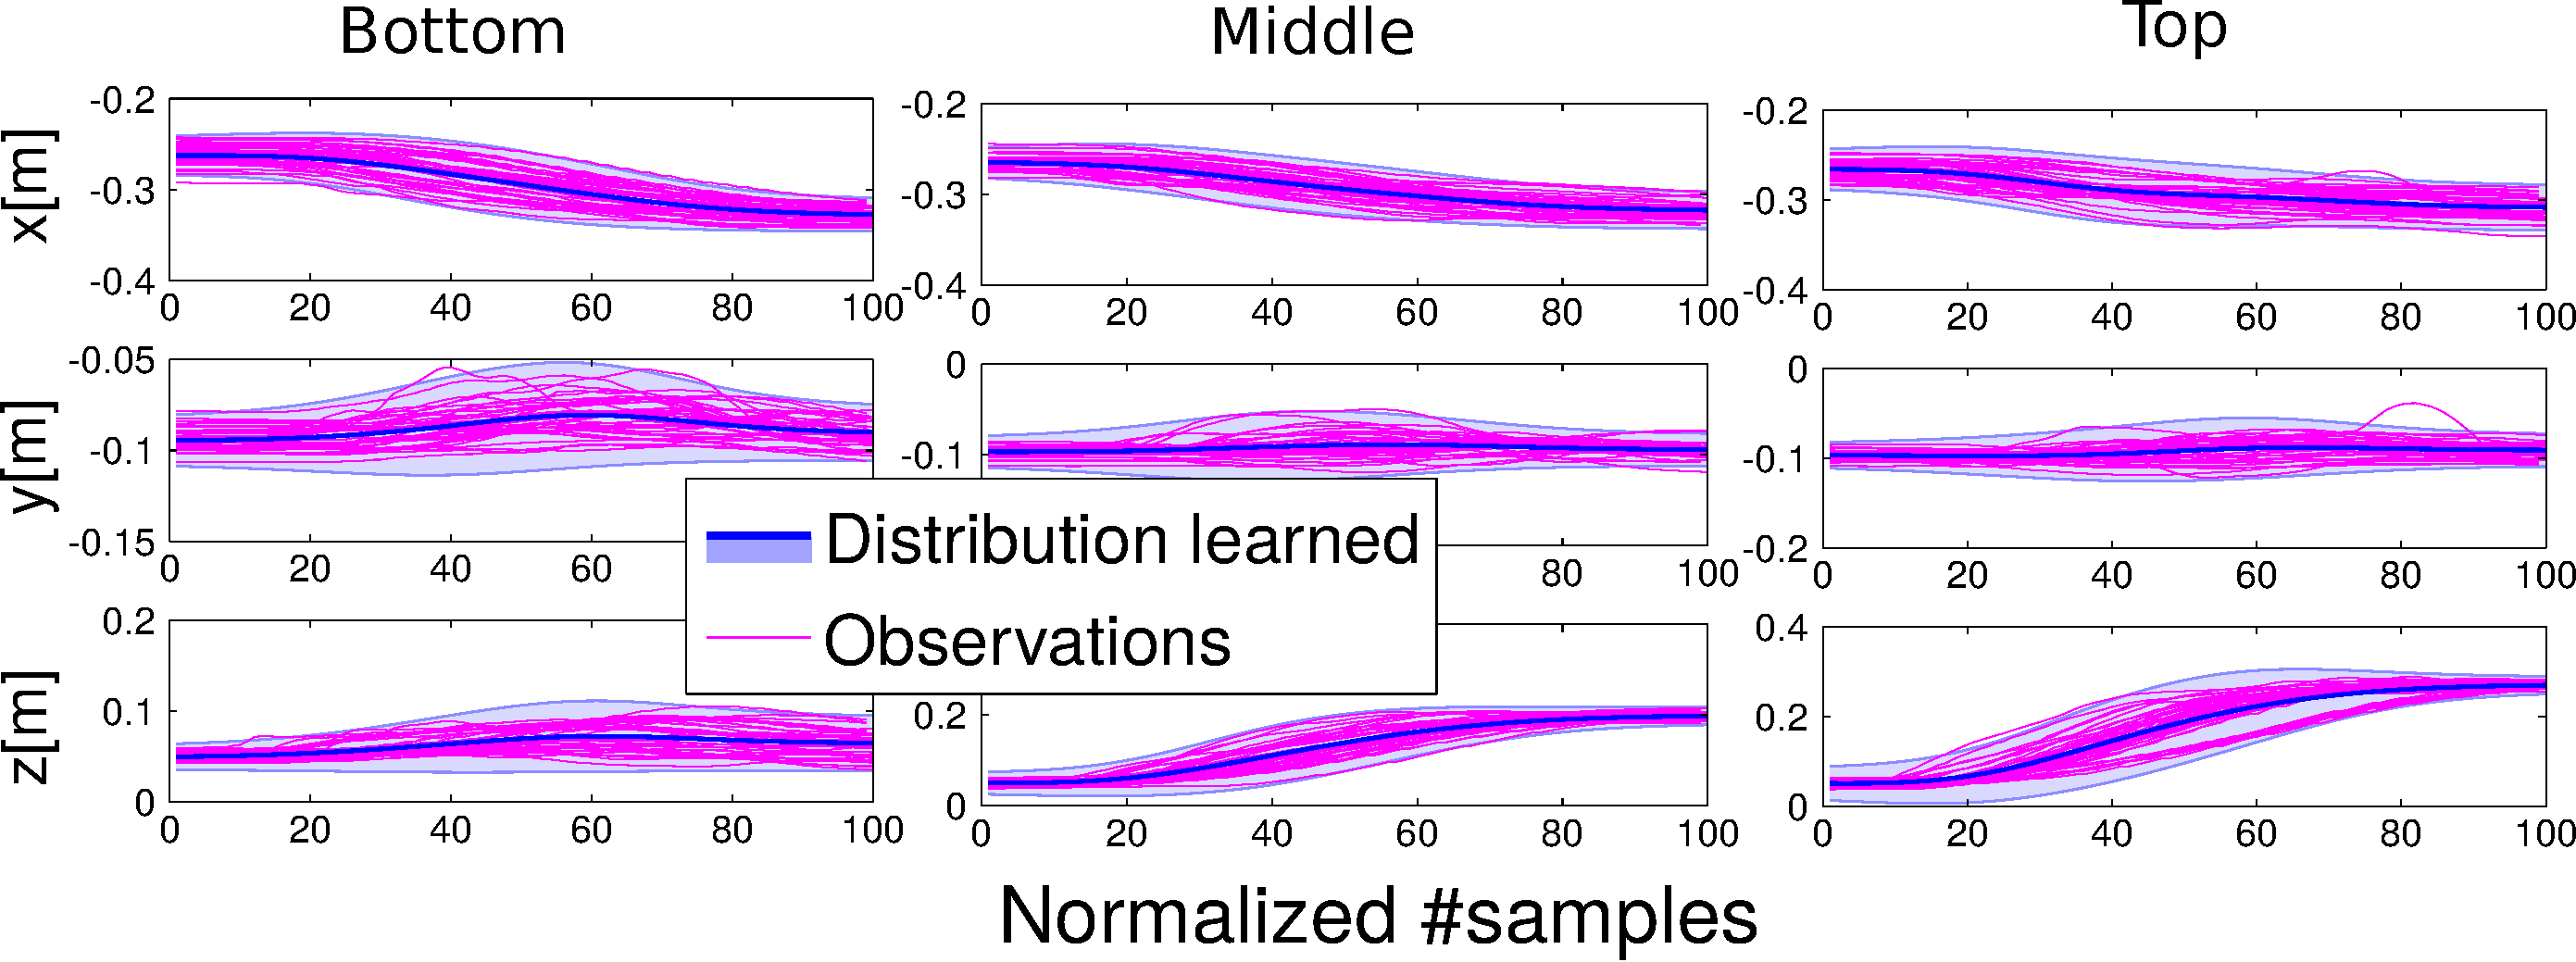
\includegraphics[width=\hsize]{img/3DOFtrajectoriesProMPsAll.pdf}\\
%}
%\caption{The ProMPs of the three different demonstrated tasks, from $39$ trajectory observations per ProMP; with M=5 basis functions per information learned; $c={1 \over M}, h={1 \over M^2}$ the parameters of the \textit{RBFs}' Gaussians, $\bar{s} = 100$ the reference number of samples. Note that we represent only the Cartesian position without force information to be readable.}
%\label{fig:3TargetsTrajectoriesProMP}
%\end{figure}
\begin{figure}[h]
\centering
{
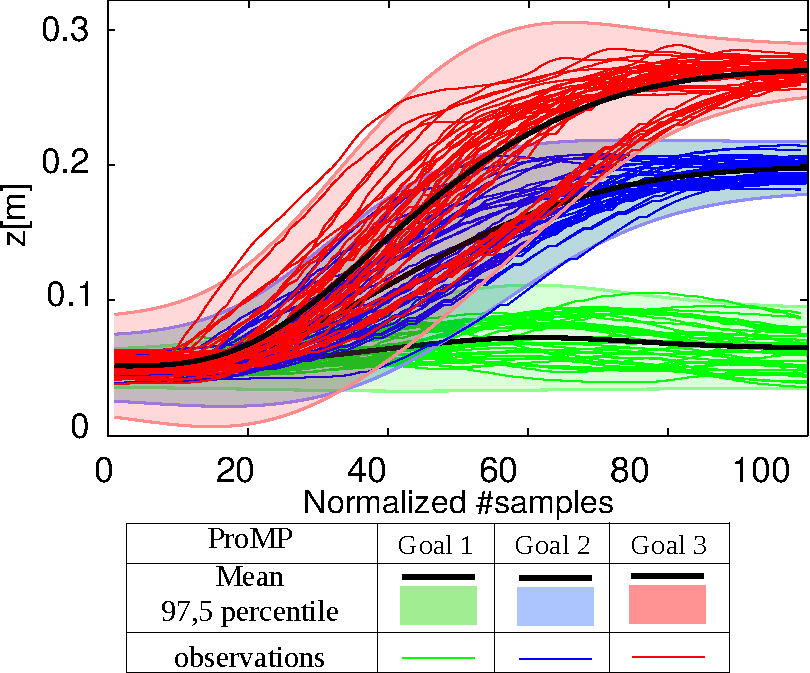
\includegraphics[height=8cm]{img/3DOFtrajectoriesProMPs.pdf}
}
\caption{Axe $z$ de la position Cartésienne pour les trois \textit{ProMPs} permettant d'atteindre des buts positionnées à différentes hauteurs. Il y a $39$ trajectoire de démonstration pour chaque \textit{ProMP} avec $M=5$ fonctions à base radiale (ici des Gaussiennes), paramétrées par $c={1 \over M}, h={1 \over M^2}$ et $\bar{s} = 100$.}
\label{fig:3TargetsZTrajectoriesProMP}
\end{figure}


\subsection{Prédiction du mouvement désiré}

Maintenant que les trois \textit{ProMPs} sont apprises, la prédiction de la fin de la trajectoire peut être effectuée, à partir de $n_o$ observations initiales.
Ce nombre est calculé à partir de la variable présentée précédement \mcode{percentData} : $n_o= |{percentData \over 100}* t_{fi}|$, où $i$ est l'indexe de la trajectoire test.

Afin de préparer la prédiction, le paramètre de modulation du temps de chaque trajectoire est calculé à l'aide d'une modélisation :
\begin{lstlisting}
    w = computeAlpha(test.nbData,t, nbInput);
    promp{1}.w_alpha= w{1};
    promp{2}.w_alpha= w{2};
    promp{3}.w_alpha= w{3};
\end{lstlisting}
Cette modélisation s'appuie sur la \toimprove{variation brutale} de la position Cartésienne durant les $n_o$ premières observations. Les calculs effectués par cette modélisation sont expliqués dans la Section~\ref{sec:predictDuration}.

Maintenant, afin d'estimer ce paramètre de modulation du temps, il suffit d'appeler la fonction :
\begin{lstlisting}
[alphaTraj,type, x] = inferenceAlpha(promp,test{1},M,s_bar,c,h,test{1}.nbData, expNoise, 'MO');
\end{lstlisting}
où \mcode{alphaTraj} contient l'estimation du paramètre de modulation du temps $\hat{\alpha}$ et la variable \mcode{type} correspond à l'index de la \textit{ProMP} reconnu (\textit{e.g.} le type de primitive de mouvement). Le dernier paramètre \mcode{x} est utilisé dans des buts de débogage.

% This variable vector contains the early observations of the trajectory translated with an offset to be centred at the moyenne of the recognized ProMP.  
%\marco{why the moyenne? Why this translation?}
%\rev{It is hard to explain in english for me, I join a picture to explain the idea}
En utilisant cette estimation du paramètre de modulation du temps, la fin de la trajectoire est alors inférée avec :
\begin{lstlisting}
infTraj = inference(promp, test{1}, M, s_bar, c, h, test{1}.nbData, expNoise, alphaTraj);
\end{lstlisting}
%
%It can be interesting to plot the predicted trajectories for the different targets, after few or more observations. The Figure~\ref{fig:1DOFtrajectoriesPredictions3targets} represent such plots.

%\begin{figure}[!h]
%\centering
%{
%Target: green (bottom)
%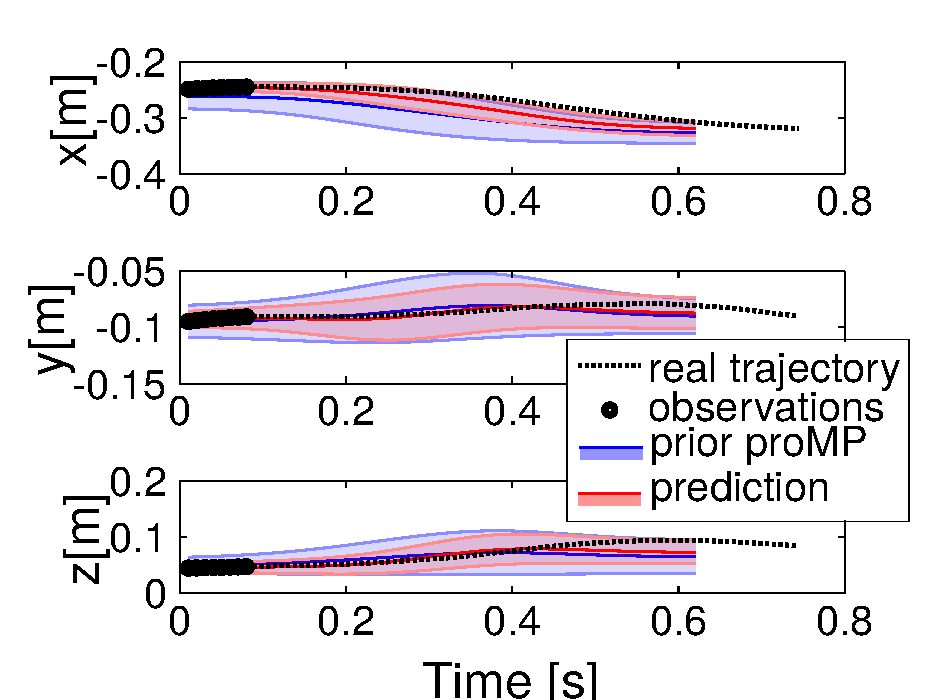
\includegraphics[width=\hsize /2]{img/infData3D/bottom10.pdf}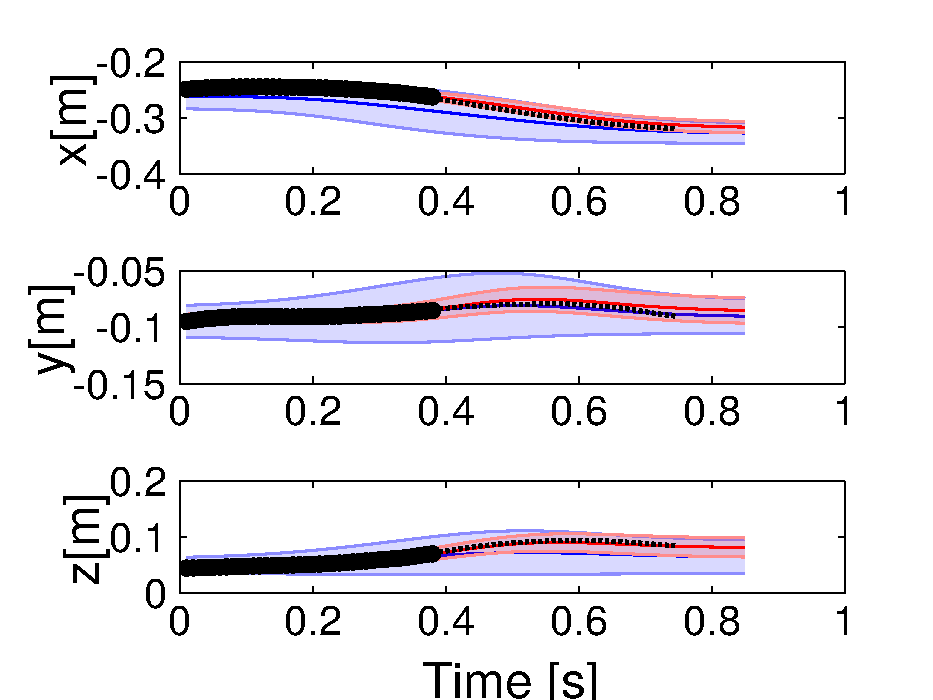
\includegraphics[width=\hsize /2]{img/infData3D/bottom50.pdf}
%%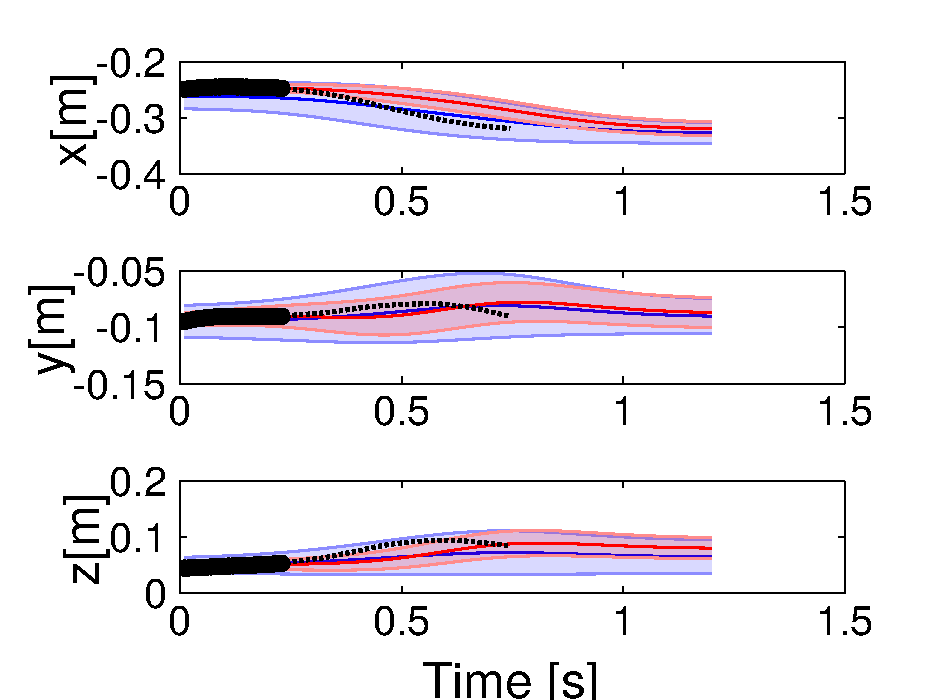
\includegraphics[width=\hsize /3]{img/infData3D/bottom30.pdf}
%Target: blue (middle)
%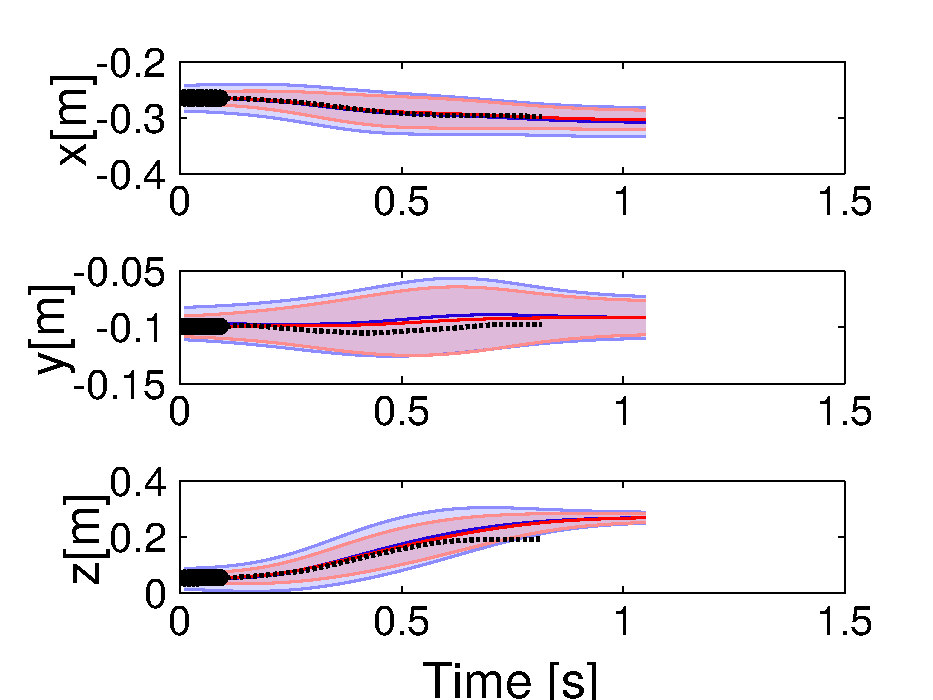
\includegraphics[width=\hsize /2]{img/infData3D/middle10Err.pdf}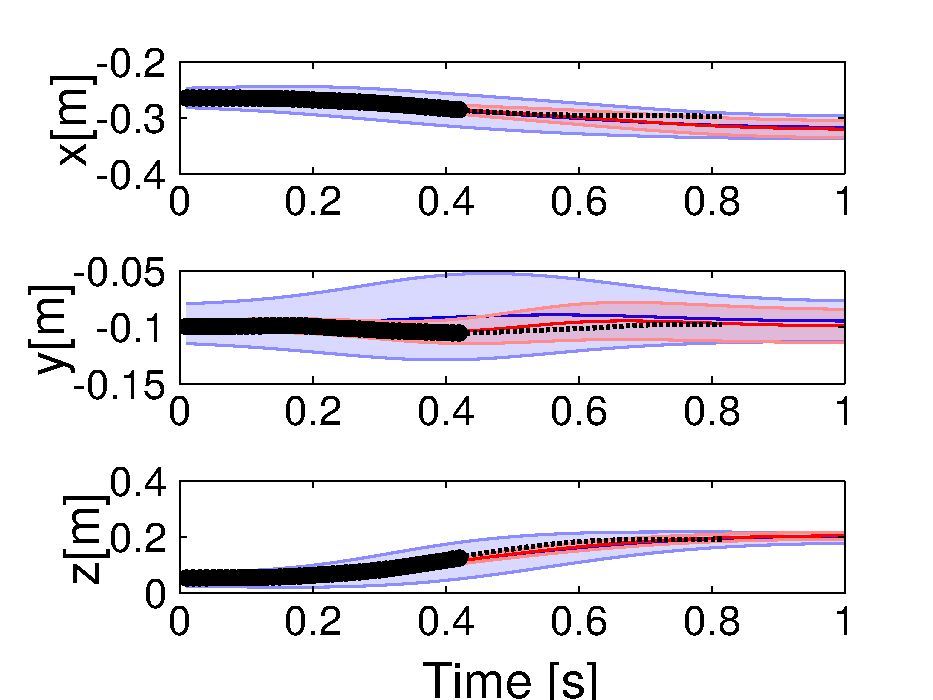
\includegraphics[width=\hsize /2]{img/infData3D/middle50.pdf}
%%%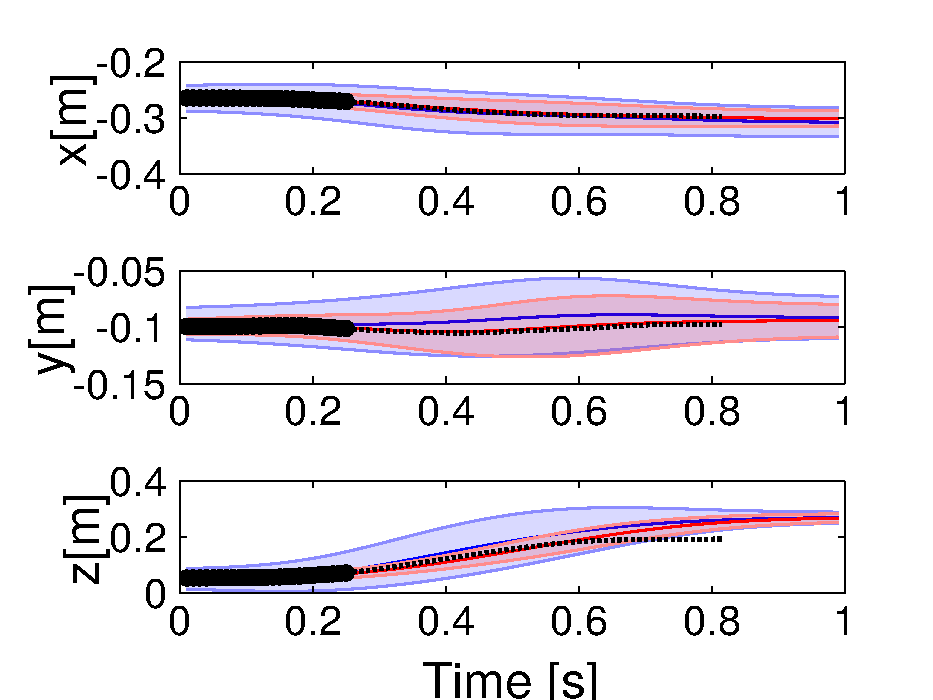
\includegraphics[width=\hsize /3]{img/infData3D/middle30Err.pdf}
%Target: red (top) 
%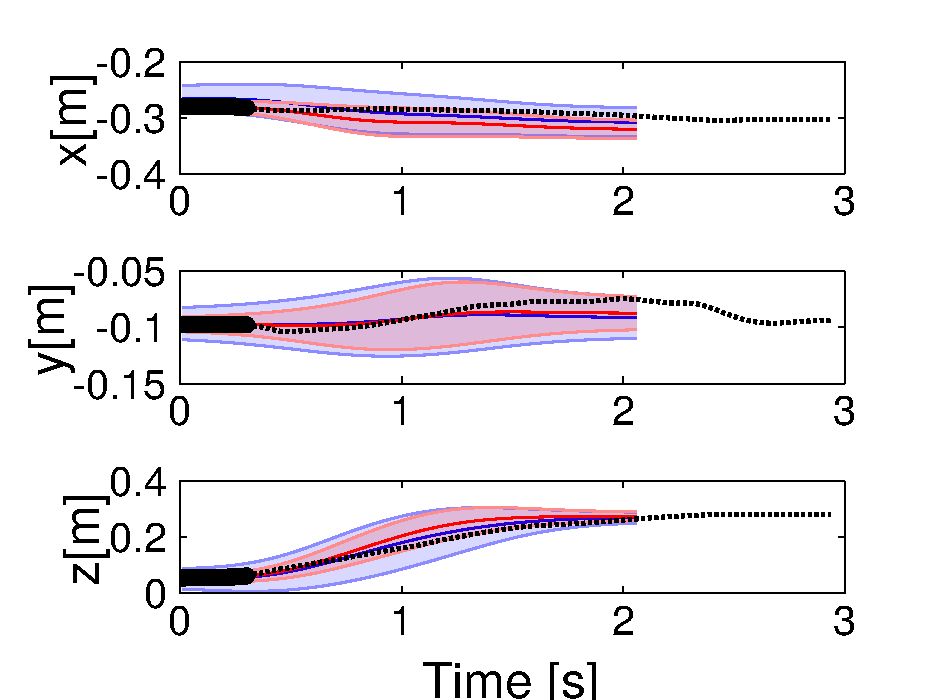
\includegraphics[width=\hsize /2]{img/infData3D/top10.pdf}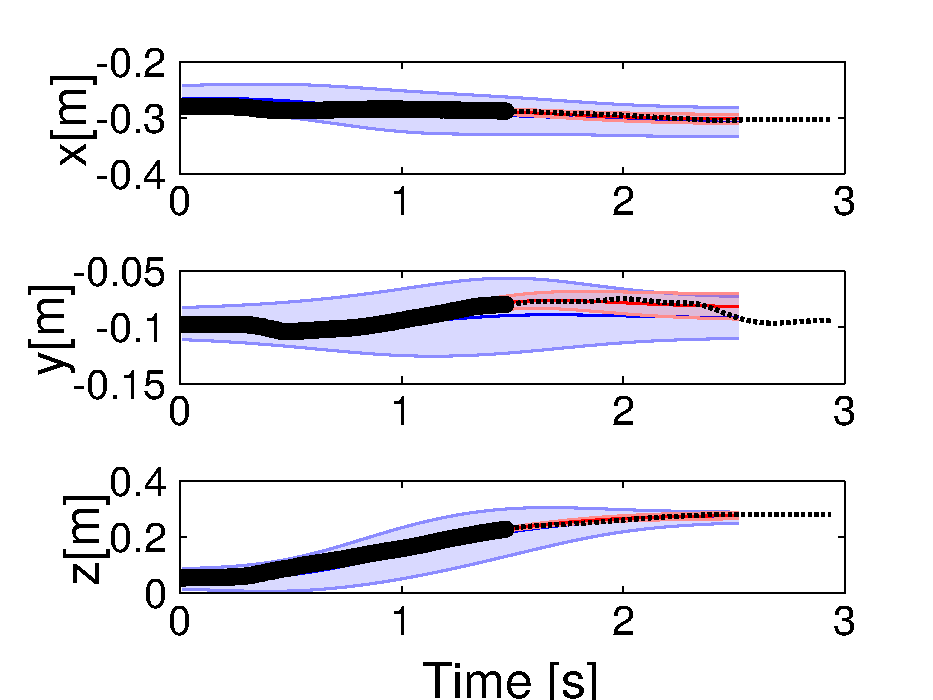
\includegraphics[width=\hsize /2]{img/infData3D/top50.pdf}
%%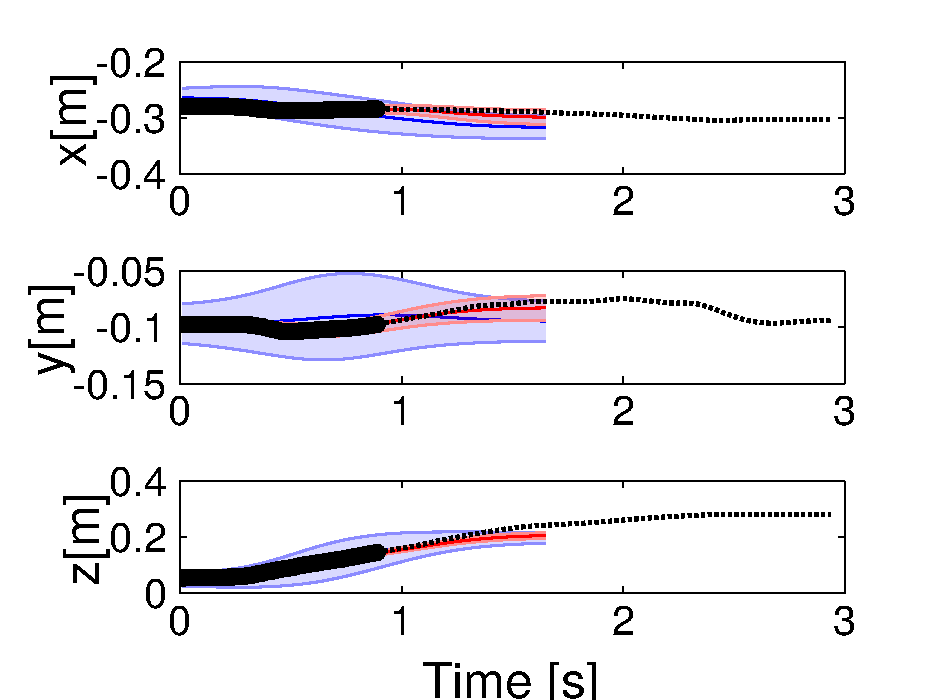
\includegraphics[width=\hsize /3]{img/infData3D/top30.pdf}
%}
%\caption{The prediction of the future trajectory thanks to the learned ProMPs computed for the  3-targets dataset (Figure \ref{fig:3TargetsZTrajectoriesProMP}) after 10 and 50 observations.}
%\label{fig:1DOFtrajectoriesPredictions3targets}
%\end{figure}

%\todo{l'image n'est pas clair, on ne voit pas grand chose : comment rendre ça plus clair ?}

Comme présenté dans l'exemple précédent, la qualité de la prédiction du future de la trajectoire dépend de la précision de l'estimation du paramètre de modulation du temps. Cette estimation est effectuée de différentes manières: 
\begin{lstlisting}
%En utilisant une modelisation :
[alphaTraj,type, x] = inferenceAlpha(promp,test{1},M,s_bar,c,h,test{1}.nbData, expNoise, 'MO');
%En utilisant un critere de distance :
[alphaTraj,type, x] = inferenceAlpha(promp,test{1},M,s_bar,c,h,test{1}.nbData, expNoise, 'DI');
%En utilisant le maximum de vraisemblance :
[alphaTraj,type, x] = inferenceAlpha(promp,test{1},M,s_bar,c,h,test{1}.nbData, expNoise, 'ML');
%En utilisant la moyenne des parametres de modulation du temps calcules lors de l'apprentissage :
alphaTraj = (promp{1}.mu_alpha + promp{2}.mu_alpha + promp{3}.mu_alpha) /3.0;  
\end{lstlisting}

%% Sere: this figure seems not correct, we better remove it
%Figure \ref{fig:3DOFtrajectoriesPredictionsDuration} shows the trajectories predicted after $n_{o}=40$ observations of a desired trajectory, with or without the prediction of the trajectory duration. The last plot shows the baseline prediction, which uses the average duration extracted from the ProMP; the other plots show the prediction using (top-left) the model of the time modulation according to the global variation of position; (top-right) the maximum likelihood that the observed trajectory is assimilated to the ProMP, tested with each $\alpha$ observed during learning; the minimum distance between the observed trajectory and each ProMP rescaled with each $\alpha$ observed during the learning.
%\begin{figure}[h]
%\centering
%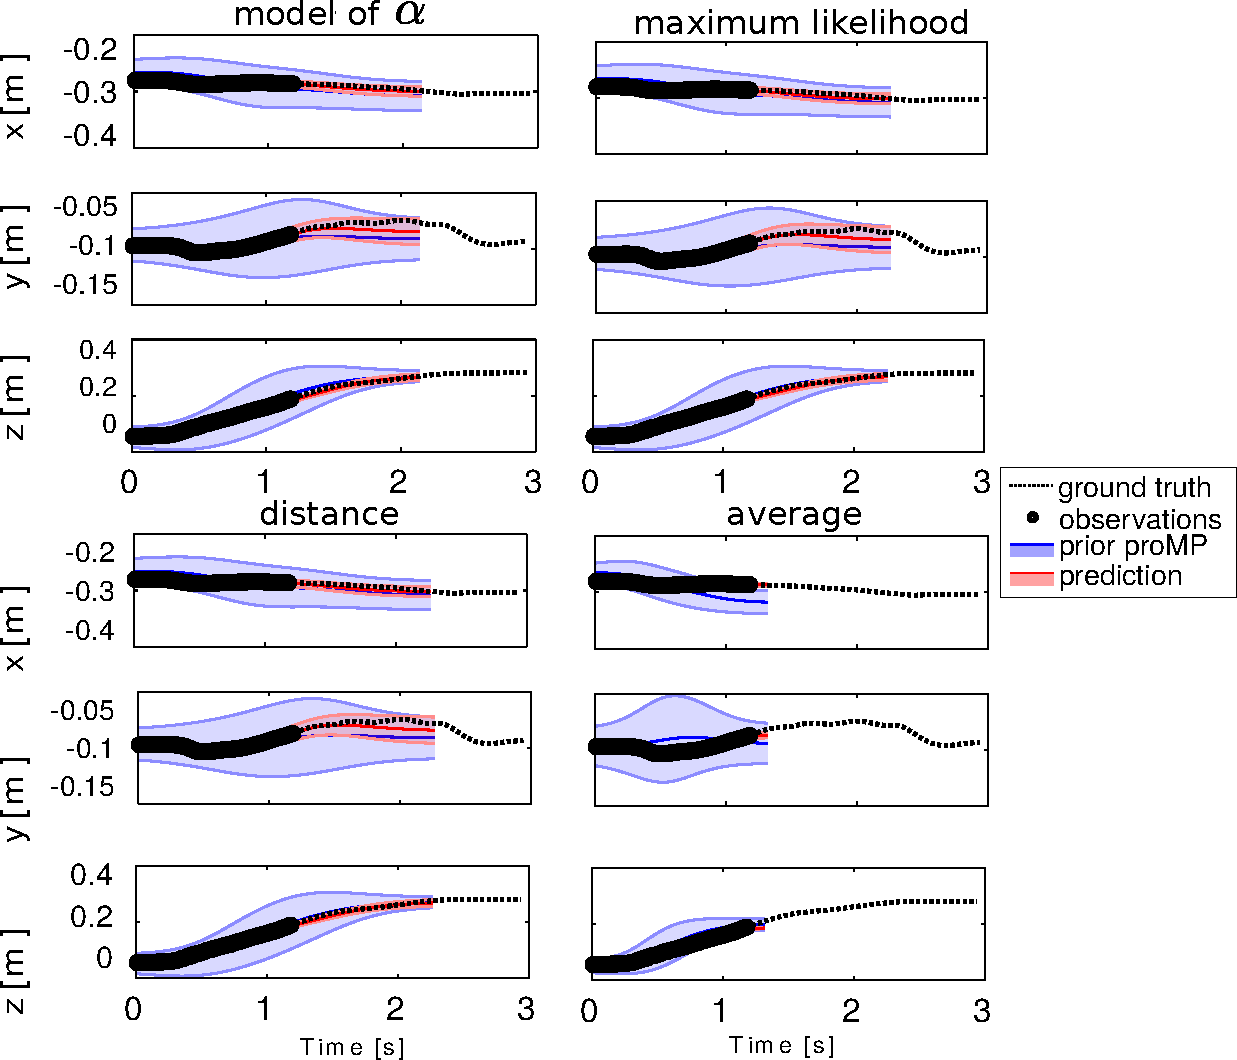
\includegraphics[height =  15cm]{img/3DOFtrajectoriesPredictionsDuration.pdf}
%\caption{The prediction of the future trajectory given $n_{o}=40$ early observations thanks to the learned ProMPs computed for the test dataset (Figure \ref{fig:3TargetsZTrajectoriesProMP}). The plots show the predicted trajectories: 1) using the model of $alpha$ according to the global position variation during the $n_o$ first observations; 2) using the maximum likelihood criteria 3) using the minimum distance criteria 4) using the average duration of the ProMP. Only one example for the red target is shown here.}
%\label{fig:3DOFtrajectoriesPredictionsDuration}
%\end{figure}

\subsection{Prédiction du paramètre de modulation du temps}\label{sec:simulatedTimeModulationModels}
La Section~\ref{sec:predictDuration} présente les quatre méthodes proposées permettant d'estimer le paramètre d'estimation du temps et précise pourquoi cette estimation est importante lors de la reconnaissance de la trajectoire. 
Dans l'expérience actuelle, ces méthodes sont maintenant comparées.

% consisting of learning three ProMPs where the final position varies in the height position ($z$-axis in Cartesian coordinates). 

%Les sections précédentes ont montrées que $40$ trajectoires ont été enregistrées par primitive de mouvement, soit un total de $120$ trajectoires. 

%We recorded 40 trajectories for each movement primitive, 
%executed by four different human participants, 
%for a total of 120 trajectories.
%, with $40$ trajectories per each movement primitive. 
%This experiment has been done with four humans, that does ten trajectories for each movement primitive. Thus, we have forty observed trajectories per movements. 

Après avoir calculé les trois \textit{ProMPs} (\textit{c.f.} section précédente), l'inférence de la finition de trajectoire est maintenant testée. Pour cela, le robot doit tout d'abord reconnaitre la \textit{ProMP} correspondante, parmi les trois apprises (\textit{c.f.} Section~\ref{sec:ManyProMP}), puis il doit estimer le paramètre de modulation du temps $\hat{\alpha}$.
%To understand how to infer a trajectory from many ProMPs, refer to Section~\ref{sec:ManyProMP}. 
La Figure~\ref{fig:analyseAlpha} représente l'erreur moyenne de l'estimation de ce paramètre $\hat{\alpha}$ à partir de $10$ tests d'inférence, en fonction du pourcentage de la trajectoire totale observé par le robot (de 30\% à 90\% de la trajectoire totale) et en fonction de la méthode utilisée. 
Ces méthodes sont celles présentées précédemment appelées ``moyenne'' (\textit{c.f.} Équation~\ref{eq:avg}), ``maximum de vraisemblance'' (\textit{c.f.} Équation~\ref{eq:ml}), ``distance minimum'' (Équation~\ref{eq:minDist}) ou modélisation (\textit{c.f.} Équation~\ref{eq:model}). 
À chaque fois, la trajectoire testée est choisie aléatoirement de l'ensemble des trajectoires observées (cette trajectoire test n'est pas incluse dans l'ensemble de trajectoire de démonstration, afin qu'elle ne soit pas utilisée dans l'étape d'apprentissage). 
\begin{figure}[h]
 \begin{minipage}[c]{.46\linewidth}
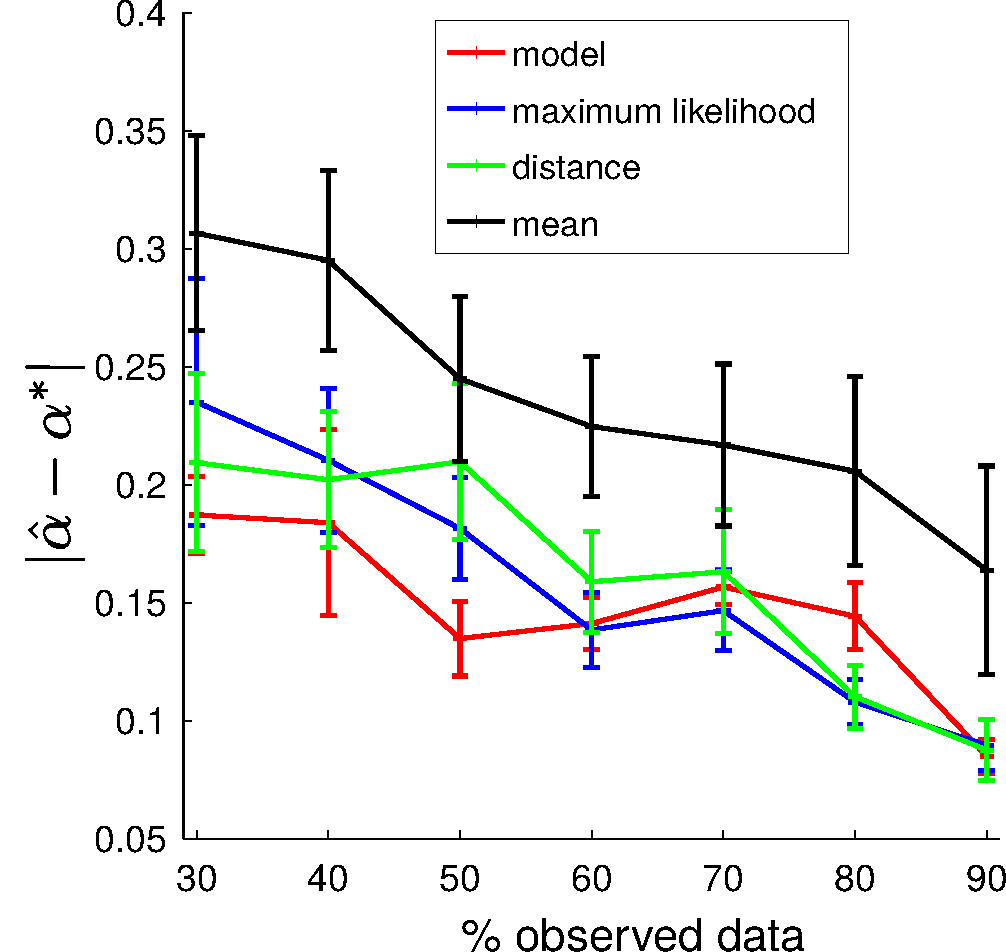
\includegraphics[width=\hsize]{img/alphaErrorAll.pdf}
\end{minipage} \hfill
  \begin{minipage}[c]{.46\linewidth}
%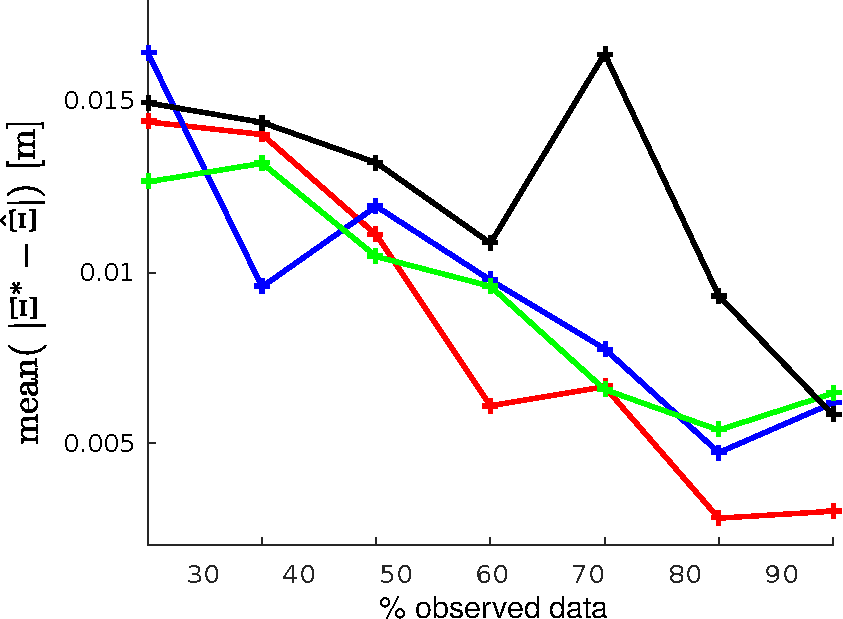
\includegraphics[width=\hsize]{img/YErrorAll.pdf}
%\center
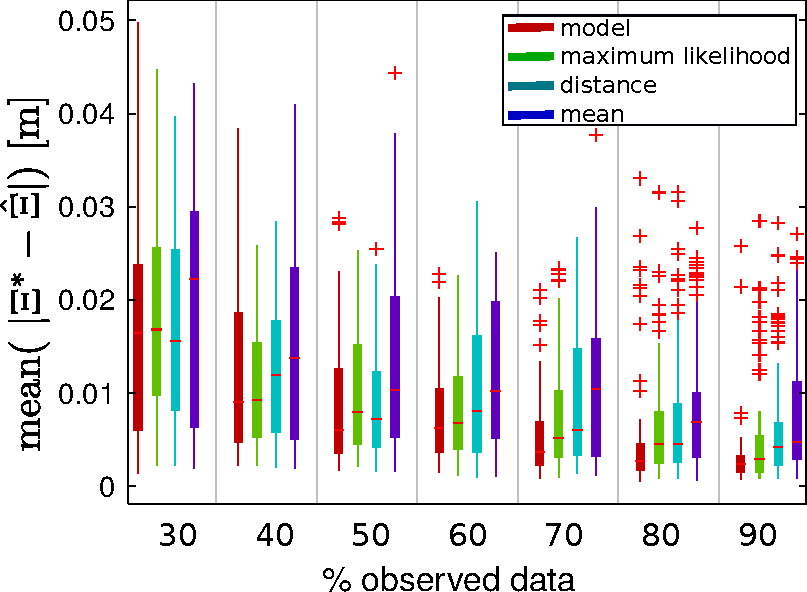
\includegraphics[height=6cm]{img/errorBoxplot.pdf}
\end{minipage}
\caption{(à gauche) Erreur d'estimation du paramètre $\alpha$  ; (à droite) erreur de la prédiction de la trajectoire, suivant le nombre d'observation connues par le robot et la méthode utilisée. Dans chaque cas, $10$ tests sont effectués.}
\label{fig:analyseAlpha}
\end{figure}
La méthode qui consiste à effectuer la moyenne des paramètres $\alpha$ observés lors de l'apprentissage est utilisée \toimprove{en comparaison} (présentée dans les graphes en noir). Les graphes mettent en avant que les autres méthodes sont plus précise. 
%La méthode du maximum de vraisemblance est plus précise, comme attendu. 
La dernière méthode (\textit{c.à.d.} celle qui consiste à modéliser le paramètre $\alpha$ en fonction de \toimprove{la variation globale} de la position Cartésienne durant les premières observations de la trajectoire) est celle qui permet au mieux d'approximer le paramètre de modulation du temps lorsque le robot observe peut de données de la trajectoire (\textit{e.g.}, 30\%-50\% observation de la trajectoire totale).  De plus, c'est cette même méthode qui infère le mieux la trajectoire désirée. Ainsi, on utilise la méthode de la \textit{modélisation} pour nos expériences, quand il s'agit de reconnaître la trajectoire à partir de la position Cartésienne du robot.
%Note that even though 



%\newpage
%%%%%%%%%%%%%%%%%%%%%%%%%%%%%%%%%%%%%%%%%%%%%%%%%%%%%%%%%%%%%%%%%%%%%%%%%%%%%%%%
\section{Application sur le robot \textit{iCub} réel}
\label{sec:appliRealIcub}

Dans cette section, nous nous intéressons à deux expériences effectuées sur le robot \textit{iCub} réel.

La première expérience s'inspire de l'expérience précédente (\textit{c.f.} Section \ref{sec:3ProMPsAppli}), où les  ``tâches'' sont représentées par des trajectoires de démonstration dirigées vers des buts distincts. Ces démonstrations sont effectuées par un collaborateur humain. Cette expérience permet d'explorer comment les informations sur les forces et les couples peuvent être exploitées. 
Afin de pouvoir évaluer la qualité des prédictions, les trajectoires tests présentées partiellement au robot sont en réalité connues dans leur totalité, afin d'avoir une ``vérité terrain''.
%The task consists in collaborating with a human operator to sort objects. 

%As an example, imagine a classic object sorting scenario, where the tasks could be transferring the objects to the correct bin or tray, or an assembly scenario where the tasks are different object-picking and manipulation trajectories, to be performed with or without the human partner.
%}

La seconde expérience consiste en un scénario collaboratif plus réaliste, inspiré par le tri d'objets de manière collaboratif. 
Dans de telles application, le robot est utilisé afin de soulever des objets qui peuvent être lourds, dangereux, ou que l'humain ne peut pas manipuler (\textit{i.e.} des objets chimiques ou de la nourriture). Le partenaire humain imspecte alors l'objet et décide si il est accepté ou rejeté. Selon cette décision, l'objet est mis dans une corbeille positionné en face du robot, ou dans une poubelle placée à coté du robot. 
Jeter l'objet l'objet dans les deux cas doit être effectué de manière différente. Réaliser cette tâche avec le \textit{iCub} n'est pas évident, car son espace opérationnel est limité et il ne peut pas porter d'objets lourds. C'est pourquoi, l'expérience a été simplifié et correspond au déplacement de petits objets et de deux corbeilles. Le partenaire humain n'a qu'a commencer un mouvement en guidant le bras du robot, puis de le lâcher, le robot finit alors le mouvement à accomplir par lui même.
Pour garantir la sécurité du robot, les trajectoires prédites sont alors présentés sur une interface graphique représentant le monde du robot, puis sont validés sur le champs par l'opérateur humain afin que le robot effectuent le mouvement.

Pour des scénario de collaboration plus compliqué, les tâches pourront être des tâches élémentaires telles que pointer, attraper, atteindre, manipuler des objets. Dans cette étude, nous n'avons pas effectué ce type de tâche, cette partie n'étant pas intéressante, puisqu'elle peut être lancé directement avec le type de primitive de mouvement reconnu.

\subsection{Trois actions simples, avec informations sur les forces et les couples}
\comment{torseur = forces + moment de couple}
Dans cet exemple, les trajectoires sont aussi définies par des informations sur les forces et les couples reçus par le robot. Cet ajout de données est utile pour représenter des primitives de mouvements collaboratives puisque cela permet au robot de prendre en compte l'interaction physique qu'il a avec son utilisateur.
Contrairement aux expériences simulées, les forces et couples inférés $\hat{F}_t$ correspondent à ceux que le robot devrait percevoir si le partenaire le guide manuellement durant l'ensemble du mouvement. En effet, ces données sont calculées à partir des trajectoires de démonstrations, où l'utilisateur guide le robot pour lui permettre d'apprendre les différentes primitives de mouvement. 
Les forces et couples qui sont prédits peuvent être utilisés de différente manière en fonction de l'application.
%Par exemple, si le partenaire brise le contact avec le robot, les forces et couples perçus vont changer. Si le robot n'est pas équipé de capteurs tactiles ou de contact, ces informations peuvent alors être utilisées afin qu'il  ``perçoive'' que ce contact a été stopé et qu'il puisse l'interpréter, par exemple, comme le signe que le partenaire souhaite qu'il continue la tâche par lui meme. 
Par exemple, le robot peut utiliser ces informations afin de détecter des forces anormales qui lui sont appliqués pendant son mouvement : il pourrait alors adapter son mouvement à de nouveaux environemments (évitement d'obstacle) ou comprendre qu'il doit apprendre de nouvelles trajectoires (le partenaire reprend le controle pour lui apprendre un nouveau mouvement).
%Here, they are simply used to detect when the partner breaks the contact with the robot, and the latter must continue the movement on its own.
%In the current case where the partner let go of the robot, the forces will be weaker. Thus, in future work, if wrenches are stronger that the inferred forces, the robot will stop its action and follow the partner's guidance.

Les prochains paragraphes permettent de présenter la réalisation de l'expérience, qui consiste donc à prédire l'intention de l'utilisateur lorsque celui-ci utilise le robot réel.
%We tested our software on the real iCub. 
Le robot apprend trois trajectoires, représentant chacune des tâches différentes. La Figure~\ref{fig:realAppli} représente ces trajectoires, avec la première, présentée en rouge, qui démarre devant le robot et va vers la gauche (tâche A) ; la seconde, présentée en vert, qui démarre de la même position et finit en hauteur (tâche C) ; et la dernière, présentée en bleu, qui démarre en hauteur et qui finit sur la gauche, à la même position finale que la trajectoire précédente (tâche B).

Afin de fournir des démonstration des tâches, le tuteur humain utilise trois but visuels, visible virtuellemet sur le
``\textit{iCub\_GUI}'', qui est un module du robot \textit{iCub} qui présente l'état en temps réel du robot, avec des flèches représentant les forces externes reçues par le robot et des objets colorés représentant les cibles à atteindre.\todo{mettre une figure}

Les utilisateurs novices du robot \textit{iCub} ont des difficultés à manipuler le bras du robot et à lui faire exécuter des trajectoire complexes en $3D$~\cite{ivaldi2017towards}, mais après avoir effectué plusieurs mouvements, l'opérateur est capable d'effectuer correctement les mouvements.
De plus, même expérimenté, l'utilisateur peut effectuer un même mouvement de différentes façons, puisque les bras du robot sont composés de beaucoup d'articulation. Ces variations ne posent cependant pas de problème, puisque les \textit{ProMPs} prennent en compte la variabilité des démonstrations.
%We want to highlight that having variations in the starting or ending points of the trajectories is not at all a problem, since the ProMPs are able to deal with this variability.%, contrarily to other methods for synthesizing motion primitives.



%One challenge of this real-world application is that the robot's arm is not easy to handle. The user need to control all the robot's degrees of freedom with one of his hands. Moreover, the user can guide the robot in different ways, so  there is variability in movements that reach the same goal.

%Despite these difficulties, we will see that 
Ainsi, en utilisant la méthode des \textit{ProMPs} et en apprenant la position Cartésienne de l'effecteur du robot, celui-ci va être capable d'apprendre des distributions de ces trajectoires, de reconnaître la distribution liée à la trajectoire courante et d'inférer la continuation du mouvement.


\begin{figure}[h]
\centering
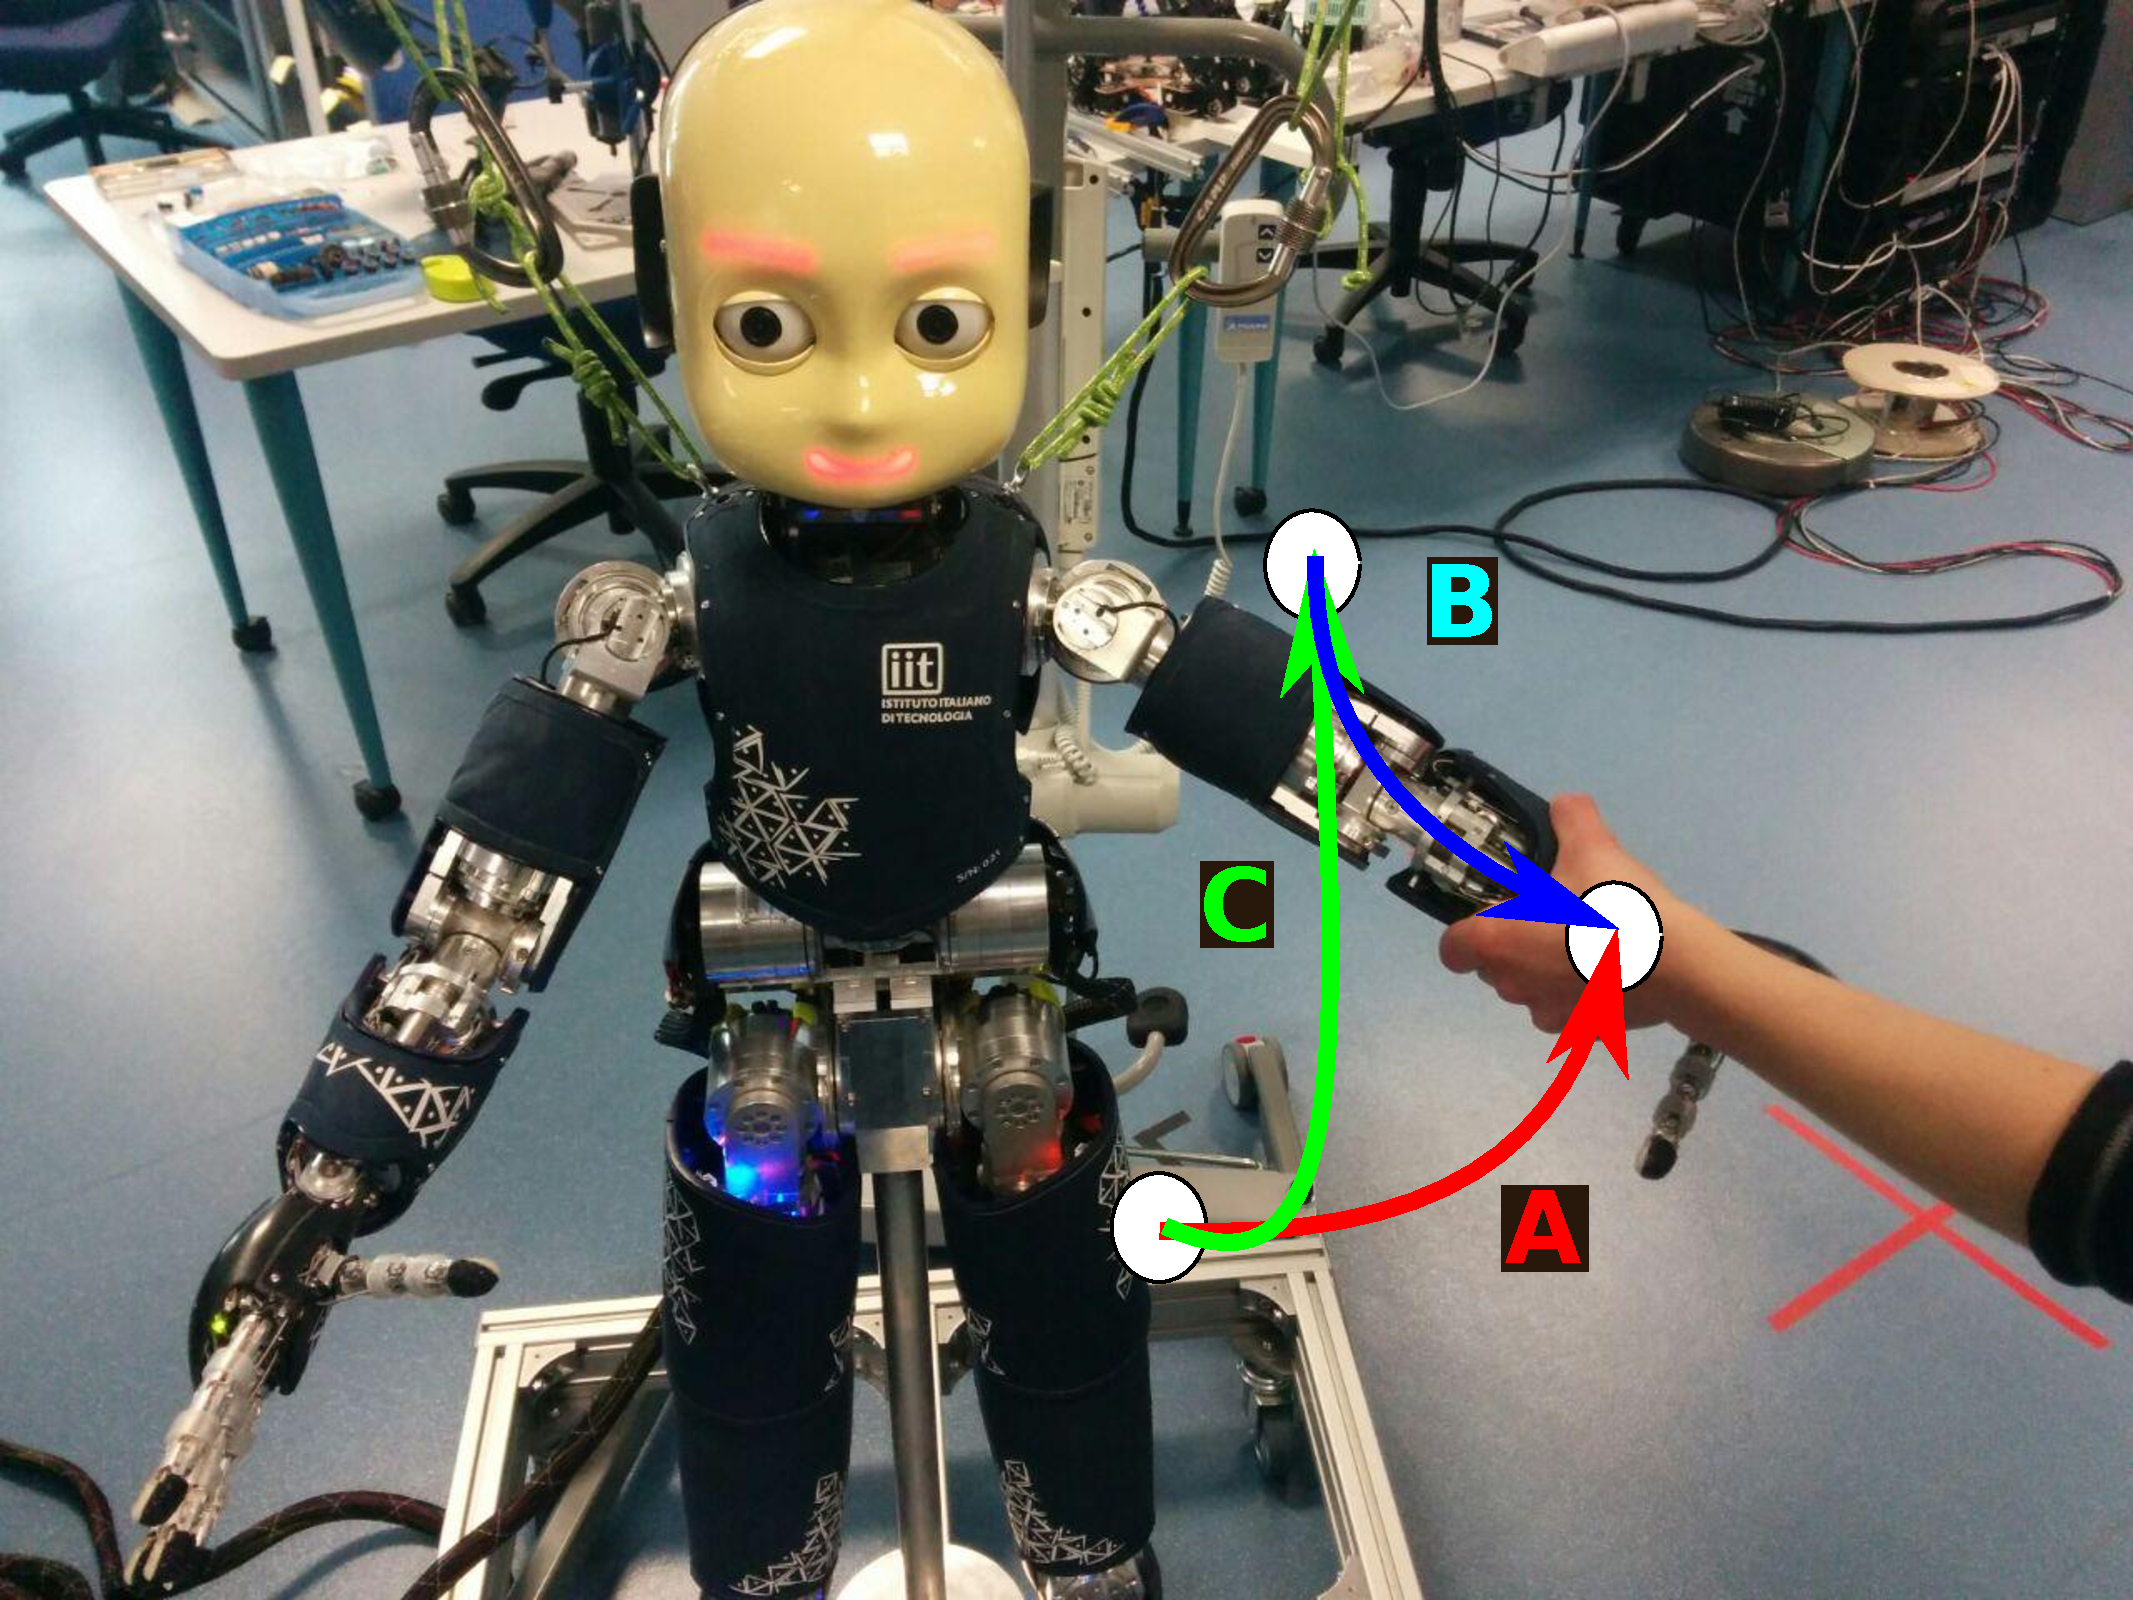
\includegraphics[width=9cm]{img/experimentRepresentation.pdf}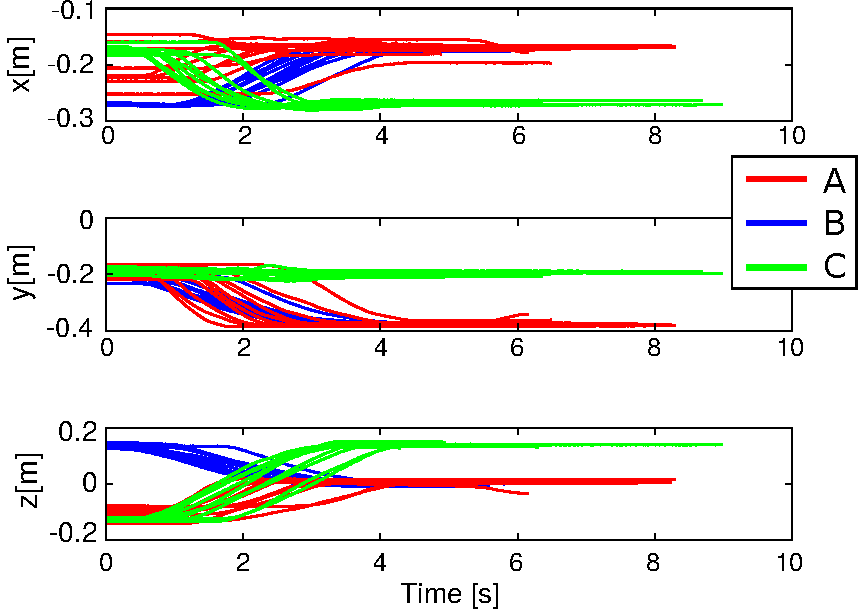
\includegraphics[width=10cm]{img/realTrajectories2.pdf}\\
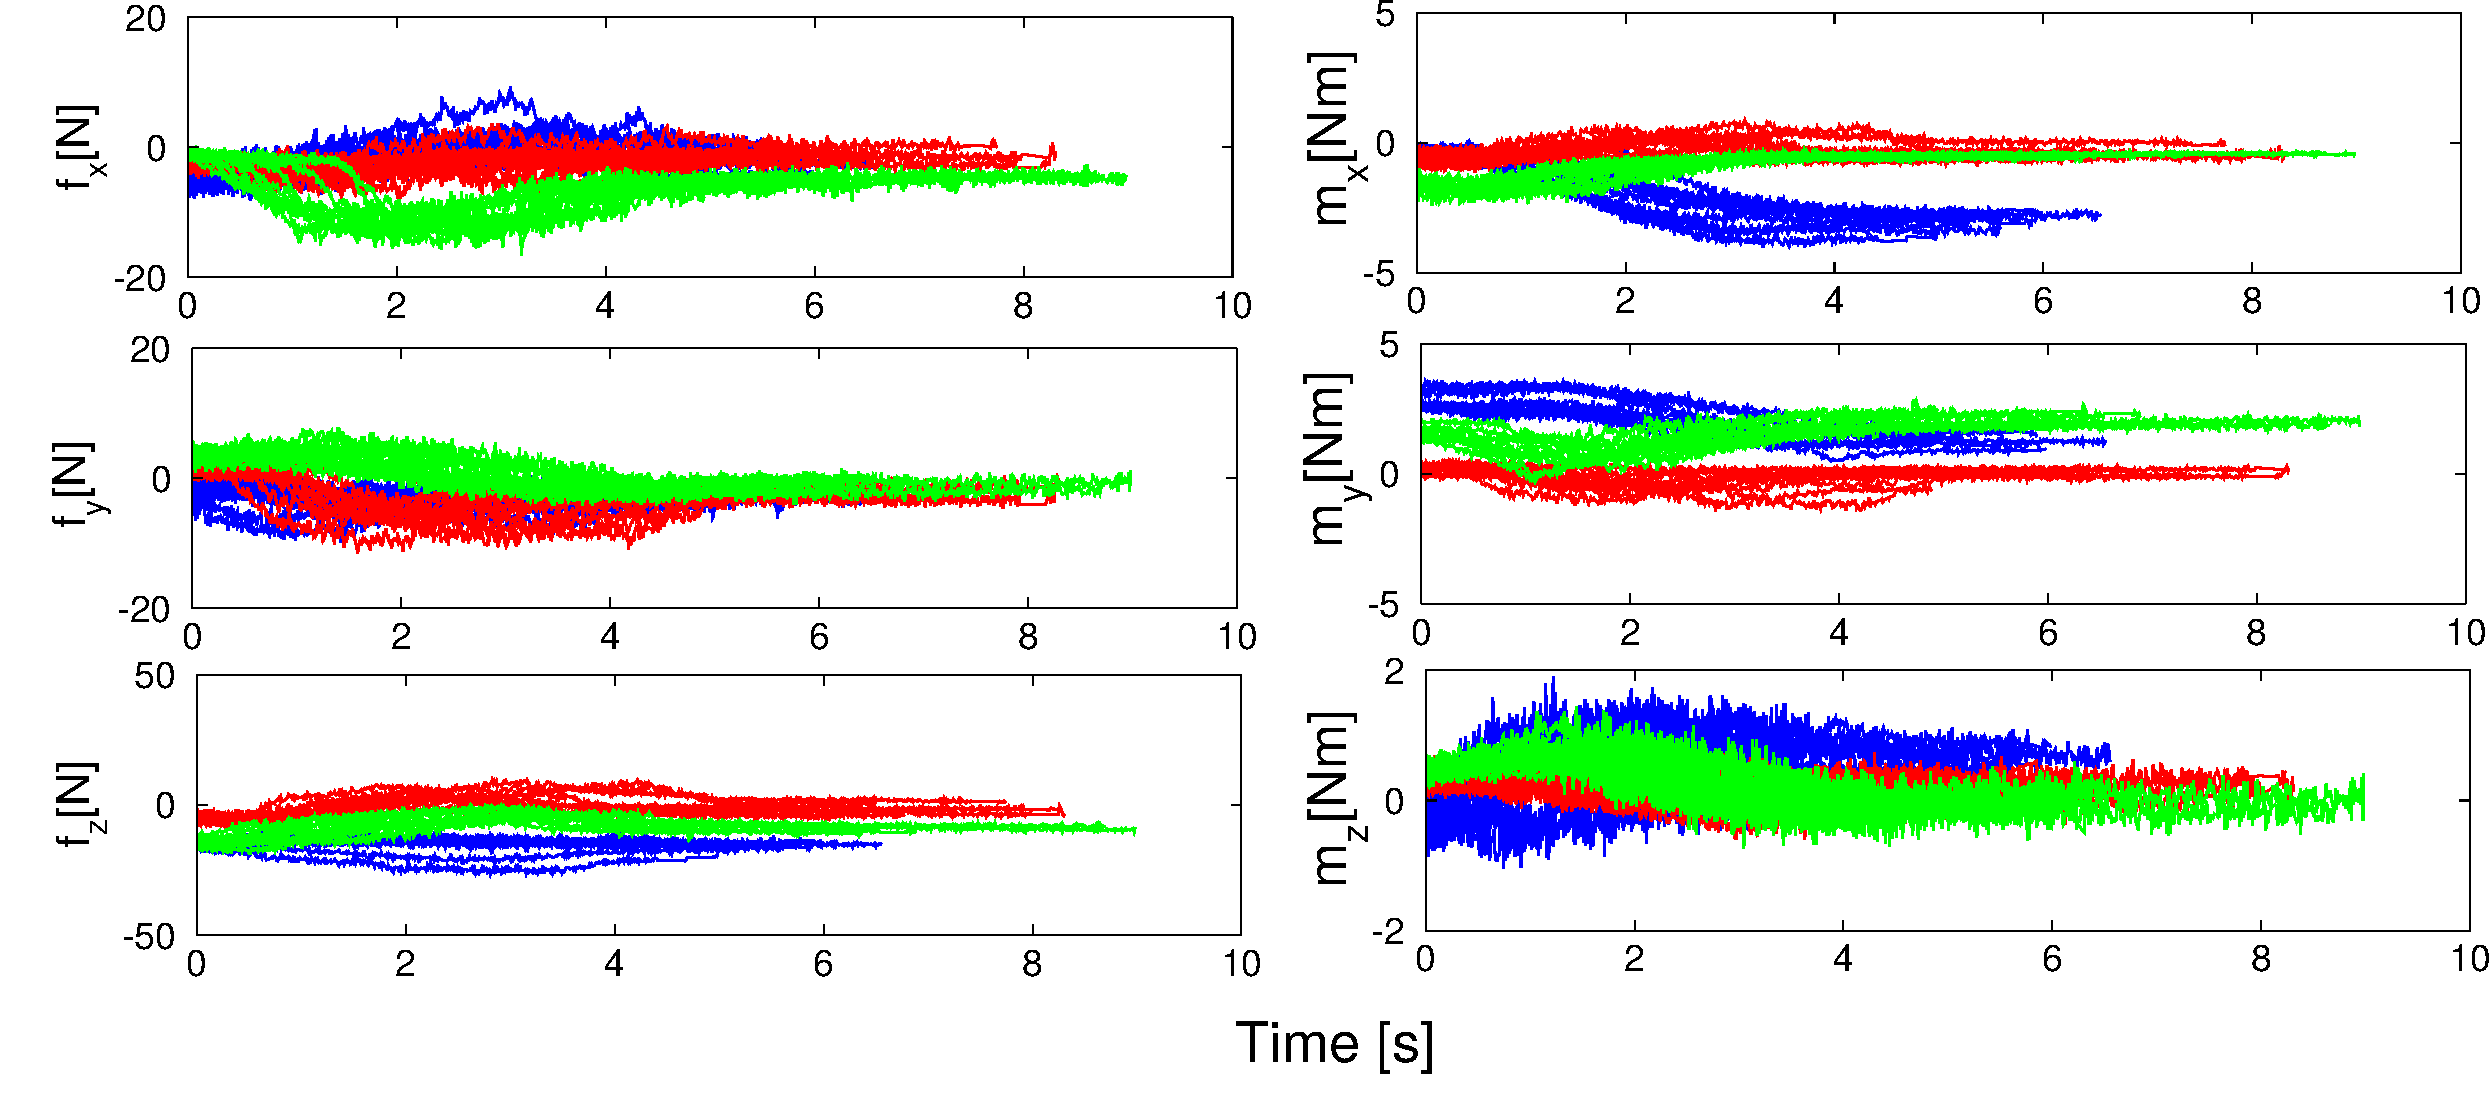
\includegraphics[width=18cm]{img/realTrajectoriesv2.pdf}
\caption{En haut à gauche : le robot \textit{iCub} et la visualisation des positions Cartésiennes des trois buts dans son espace opérationnel, avec les trajectoires correspondantes qui définissent les trois tâches A-B-C. En haut à droite : les position Cartésienne des trajectoires de démonstrations pour ces trois tâches. En bas de gauche à droite: les forces et moments des trajectoires de démonstration.
%The three trajectories presenting the primitives A, B, and C. A color code (RGB) is used throughout the paper to facilitate the recognition of trajectories (top-left); and the corresponding test-set composed of position (top) and wrench (bottom) information.
}
\label{fig:realAppli}
\end{figure}

Dans cette expérience, le robot récupère $10$ trajectoires de démonstrations par primitive de mouvement, toutes fournies par un même utilisateur. Les données enregistrées correspondent à la position Cartésienne de la main gauche du robot ainsi que les forces et moment qu'elle reçoit lors de ces mouvements. Les données sont récupérées à l'aide de la fonction \mcode{used_functions/retrieveRealDataWithoutOrientation.m}. Les paramètres de sorties de cette fonction correspondent à trois objets  (un par \textit{ProMP}) qui contiennent toutes les informations requises afin d'apprendre les \textit{ProMPs}. 
%%From these objects, the robot learned:
%Each trajectory is:
%$$\Xi_t = \begin{bmatrix}
%[x_t & y_t & z_t ]^\top \\ [F_x & F_y & F_z]^\top \\ [m_x & m_y & m_z]^\top
%\end{bmatrix}$$
%\marco{[Obs.: What did the robot learn? The parameters $\omega$ and the distributions or the trajectories?]}
%\rev{I don't understand your question: by learning the $\omega$ parameter and the distributions, the robot learns the trajectory, isn't it?} 

Dans cette fonction, les informations des forces et des couples sont filtrées à l'aide d'une fonction Matlab appelée \mcode{envelope.m}\footnote{Les informations de cette fonctions peuvent être récupérées ici : \url{https://fr.mathworks.com/help/signal/ref/envelope.html?requestedDomain=www.mathworks.com}}: pour chaque trajectoire \mcode{traj} et sa sous-matrice $M = F([1:t])$:
\begin{lstlisting}
[envHigh, envLow] = envelope(traj.M);
traj.M = (envHigh+envLow)/2;
\end{lstlisting}
Ces trois objets sont sauvegardés dans \mcode{'Data/realIcub.mat'}. Un script Matlab appelé \mcode{demo_plotProMPsIcub.m} permet de récupérer ces données, à l'aide de la fonction \mcode{load('Data/realIcub.mat')}. Ce script est organisé de la même manière que ceux présenté dans les Sections~\ref{sec:example1DOF} and \ref{sec:3ProMPsAppli}. 
En lançant ce script, les données récupérée sont d'abord représentées.

\begin{figure}[h]
\centering
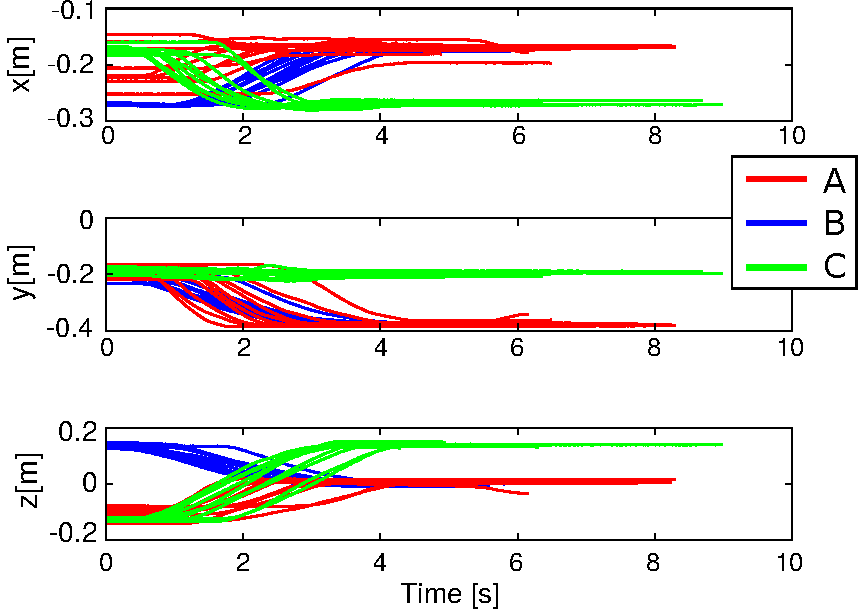
\includegraphics[height = 5cm]{img/realTrajectories2.pdf} 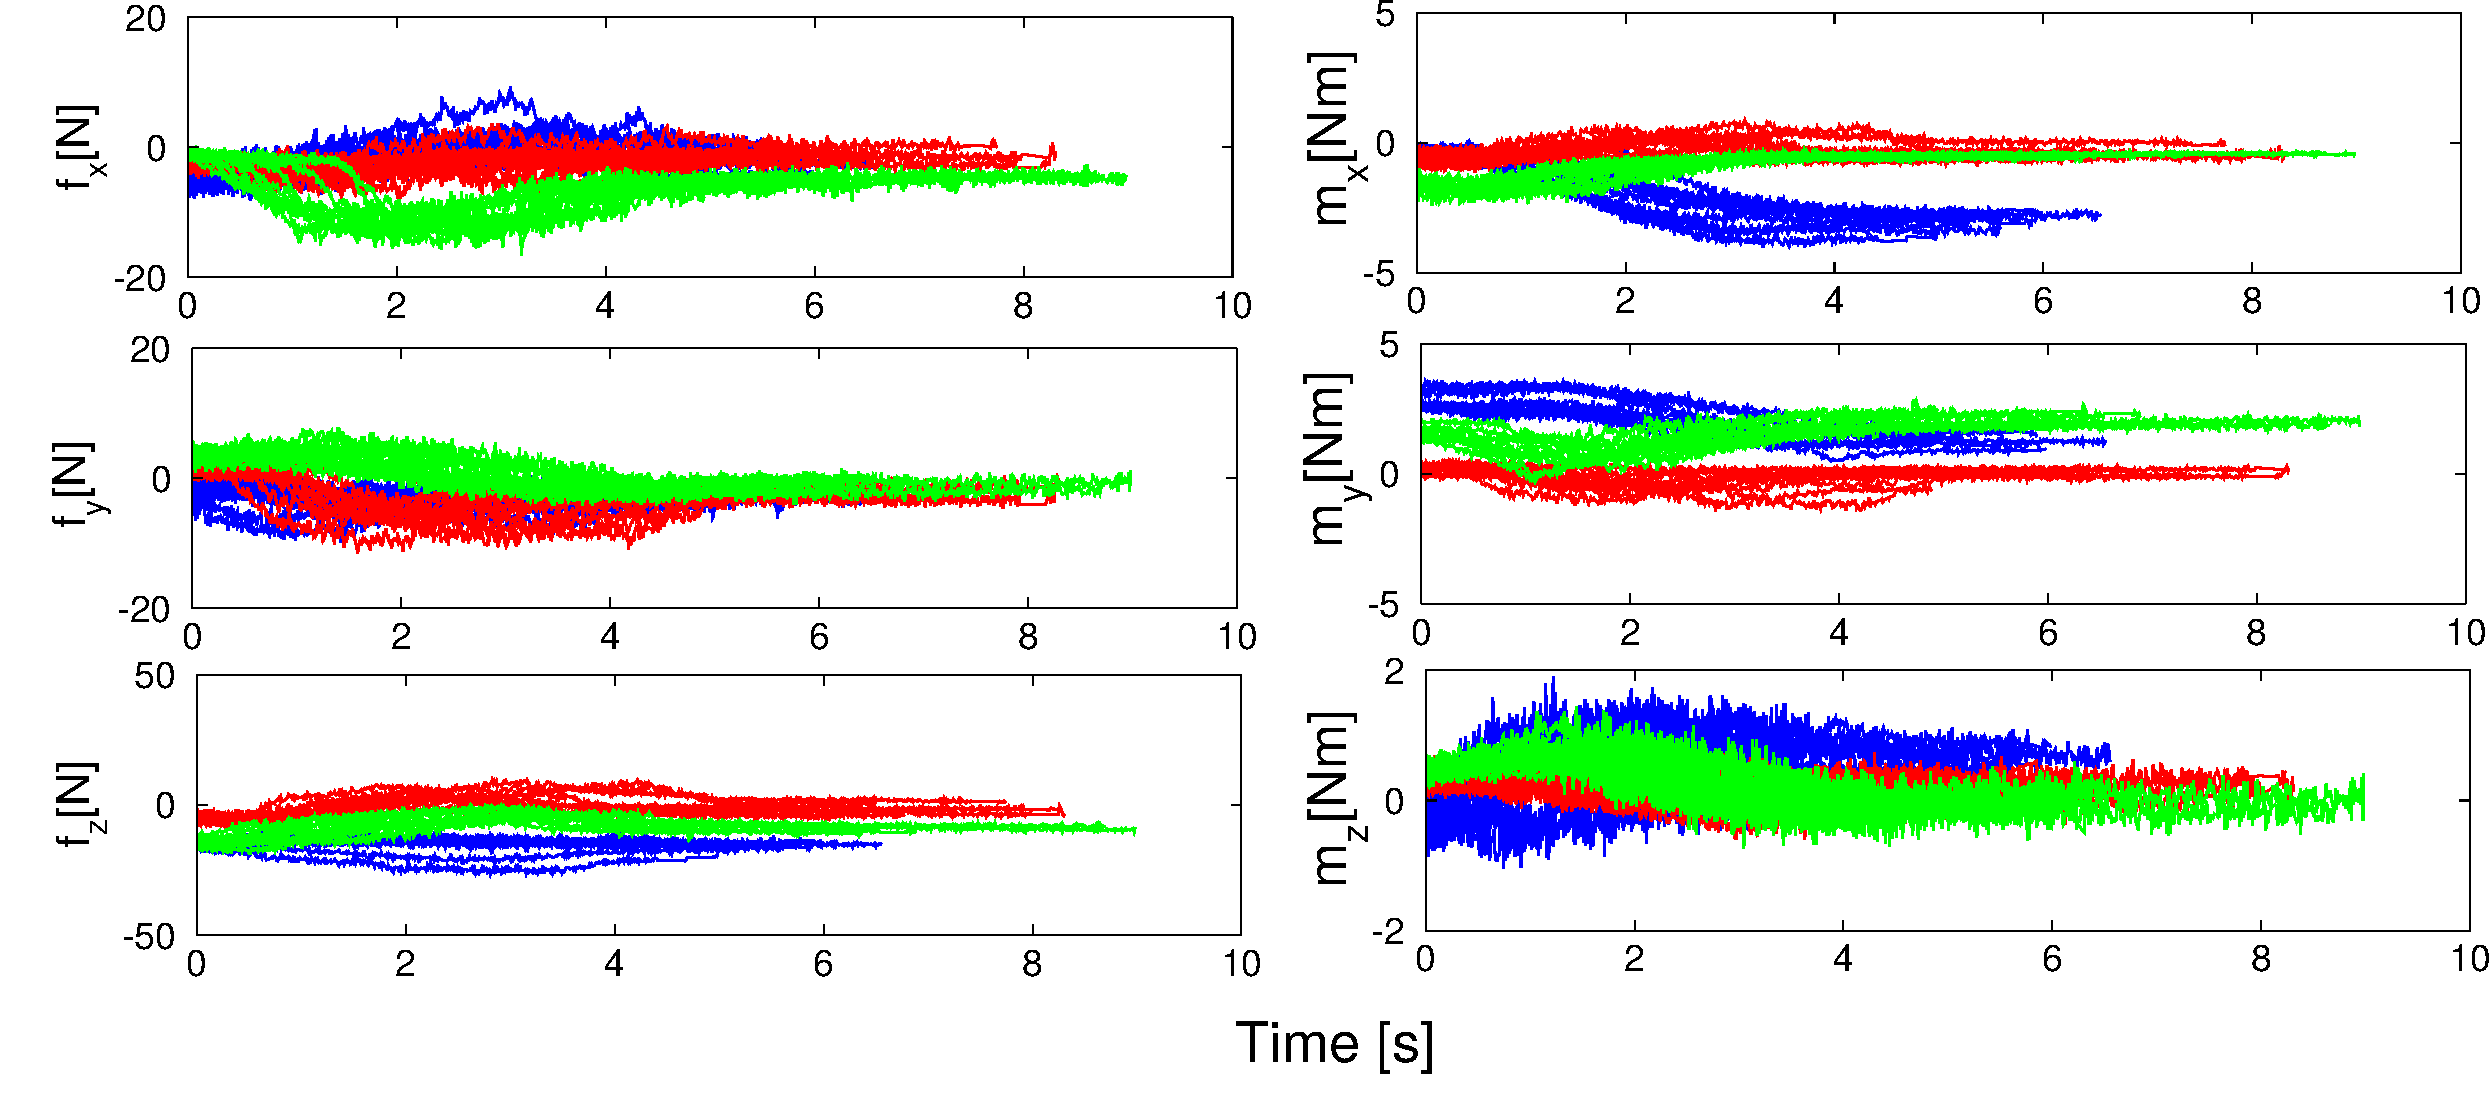
\includegraphics[width=\hsize]{img/realTrajectoriesv2.pdf} 
\caption{\ori{cette figure était supprimée.} Représentation des trois trajectoires apprises par le robot réel. En haut : position cartésienne 3D ; en bas : forces en 3D et moments en 3D.}
\label{fig:realTraj}
\end{figure}

Puis, les \textit{ProMPs} sont apprises et affichées, comme présenté dans la Figure~\ref{fig:realDistribution}.
Dans cette figure, les distributions sont visiblement superposées :
\begin{itemize}
\item le long de toutes les trajectoires en ce qui concerne les informations des couples ;
% $f_x$, $f_y$, $f_z$ and $m_z$ dimensions; 
\item lors des $40$ premiers pourcents des trajectoires en ce qui concerne l'information des positions Cartésiennes.
%$x$, $y$ and $z$ dimensions. 
\end{itemize}
%We make the hypothesis that force information is not useful for identifying trajectories. However, the robot learned it to know what are the forces' amplitude it is supposed to measure.
Après cette étape d'apprentissage, l'utilisateur choisi la \textit{ProMP} à tester. En utilisant la variable qui représente le pourcentage de données de la trajectoire que le robot observe avant d'effectuer l'inférence, le script calcul alors le nombre $n_o$ d'observations qui correspond à ce pourcentage. Notons que $n_o$ n'est pas identique pour toutes les trajectoires testées, puisque ce nombre dépend de leur durée totale. En utilisant ce nombre, le robot modélise le paramètre de modulation du temps $\alpha$ pour chaque trajectoire (\textit{c.f.} Section~\ref{sec:predictDuration}). En effet, la ``variation globale'' correspond à la variation des données de la trajectoire entre l'itération $1$ et l'itération$n_0$. En utilisant ce modèle, le paramètre de modulation du temps de la trajectoire test est estimée et la \textit{ProMP} correspondante est identifiée.

\begin{figure}[h]
\centering
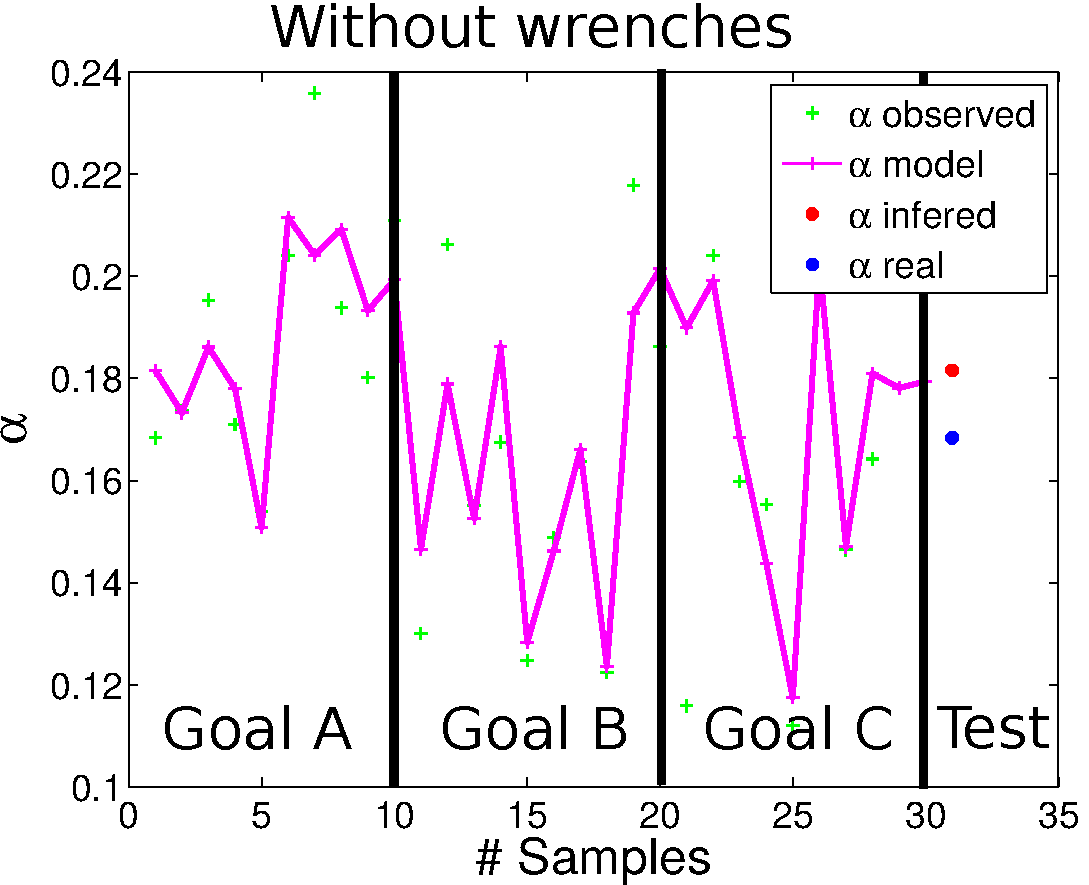
\includegraphics[width = 8cm]{img/realalphaModel.pdf} 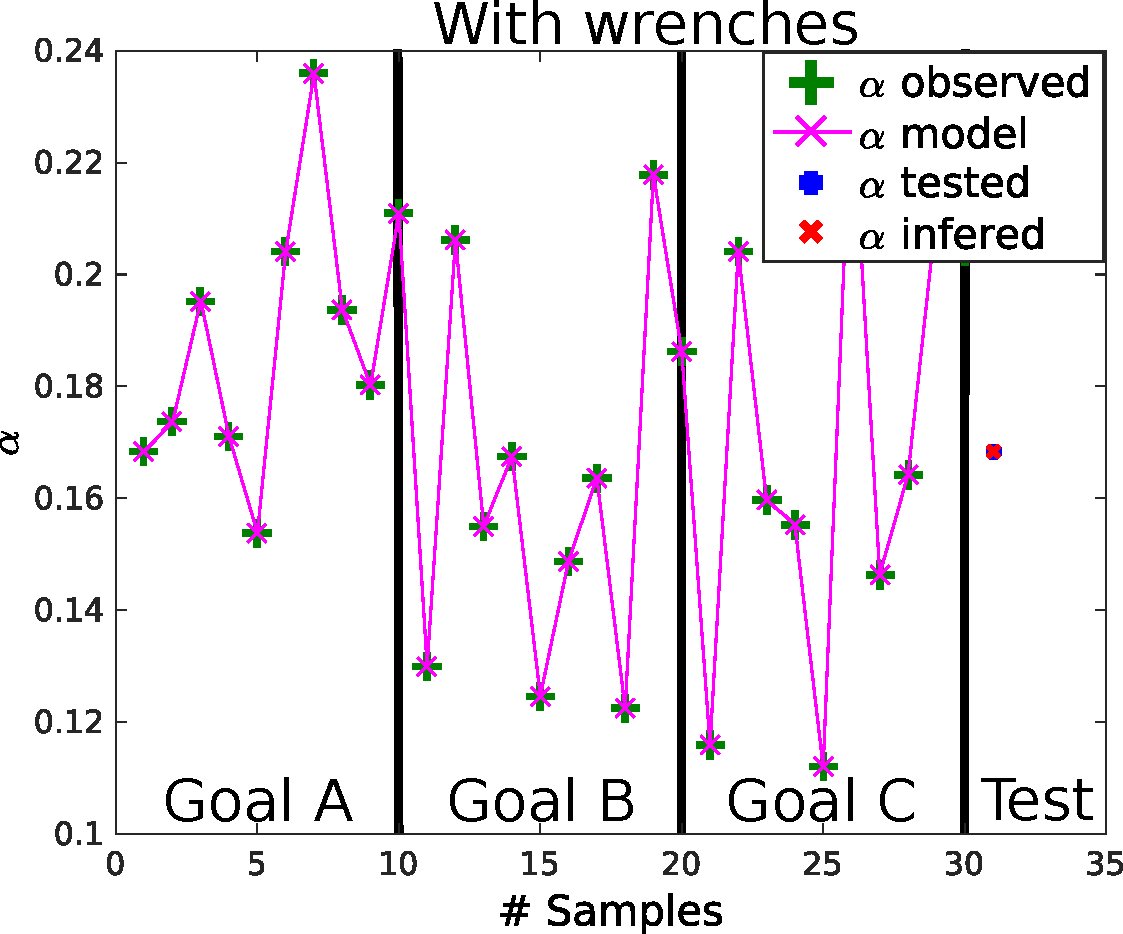
\includegraphics[width = 8cm]{img/alphaInfWithForces.pdf} 
\caption{\ori{Cette figure était supprimée}$\alpha$ model with (left) and without (right) wrenches. In pink, the $\alpha$ model based on the $\alpha$ set of the learning trajectories; in green, their real values; in red, the $\hat{\alpha}$ expectation of the test trajecory; and in blue its real value.
}
\label{fig:realalphaModel}
\end{figure}
\ori{La Figure~\ref{fig:realalphaModel} représente l'estimation de quelques paramètres $\alpha$, à l'aide de la modélisation apprise. Sur la gauche, quand la modélisation ne contient pas d'information sur les forces et les couples, et sur la droite, lorsqu'elle contient ces informations. Les croix vertes représentent l'ensemble de $\alpha$ des trajectoires d'apprentissage, et les croix roses, l'estimation effectuée par la modélisation à l'aide de cet ensemble. Les $10$ première croix correspondent à l'ensemble de $\alpha$ de la première \textit{ProMP}, les $10$ suivantes, celles de la seconde \textit{ProMP} et les $10$ dernières, celles de la dernière \textit{ProMP}. Finalement, la croix rouge correspond à l'estimation $\hat{\alpha}$ de la trajectoire testée et la croix bleue le paramètre $\alpha$ réel de cette même trajectoire. Ces résultats montre qu'avec l'information des forces et des couples, l'estimation du paramètre $\alpha$ est plus précis.}

\begin{figure}[!h]
\centering
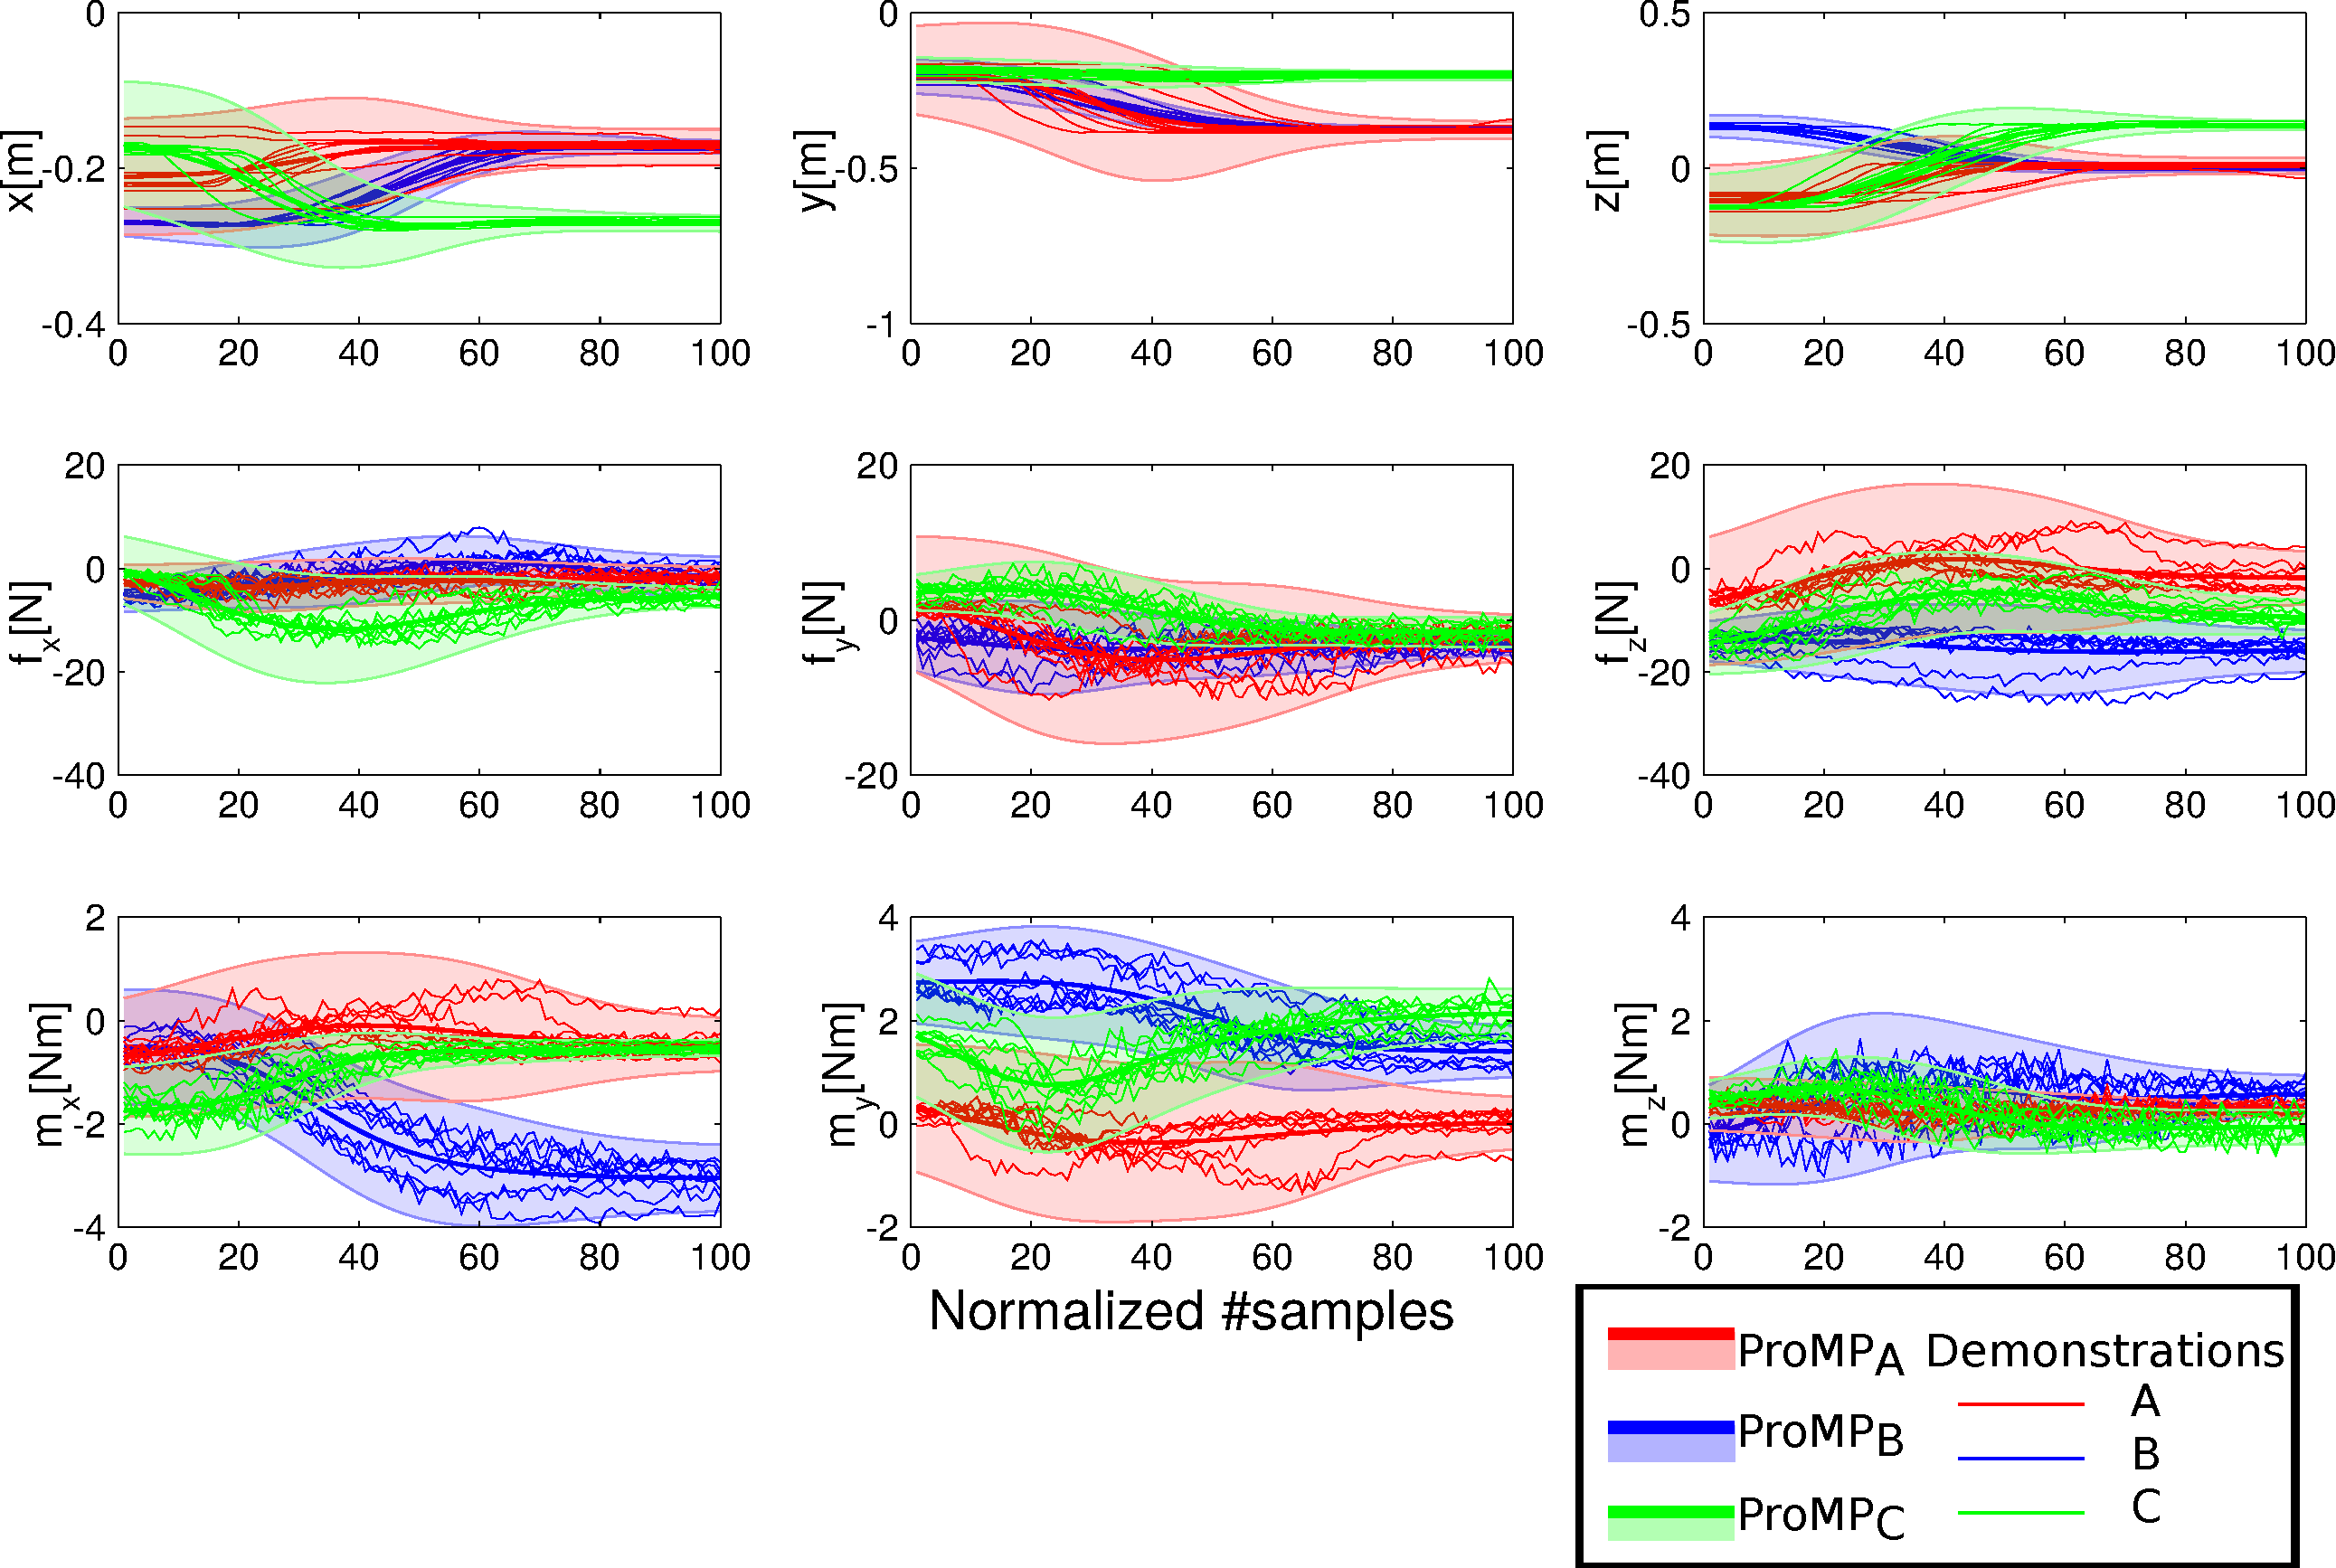
\includegraphics[height = 10cm]{img/realDistribution.pdf} 
\caption{Les \textit{ProMPs} apprises par le robot à partir des démonstrations représentées dans la Figure \ref{fig:realAppli}.}
\label{fig:realDistribution}
\end{figure}

\begin{figure}[!h]
\centering
{
\textcolor{red}{A}\\
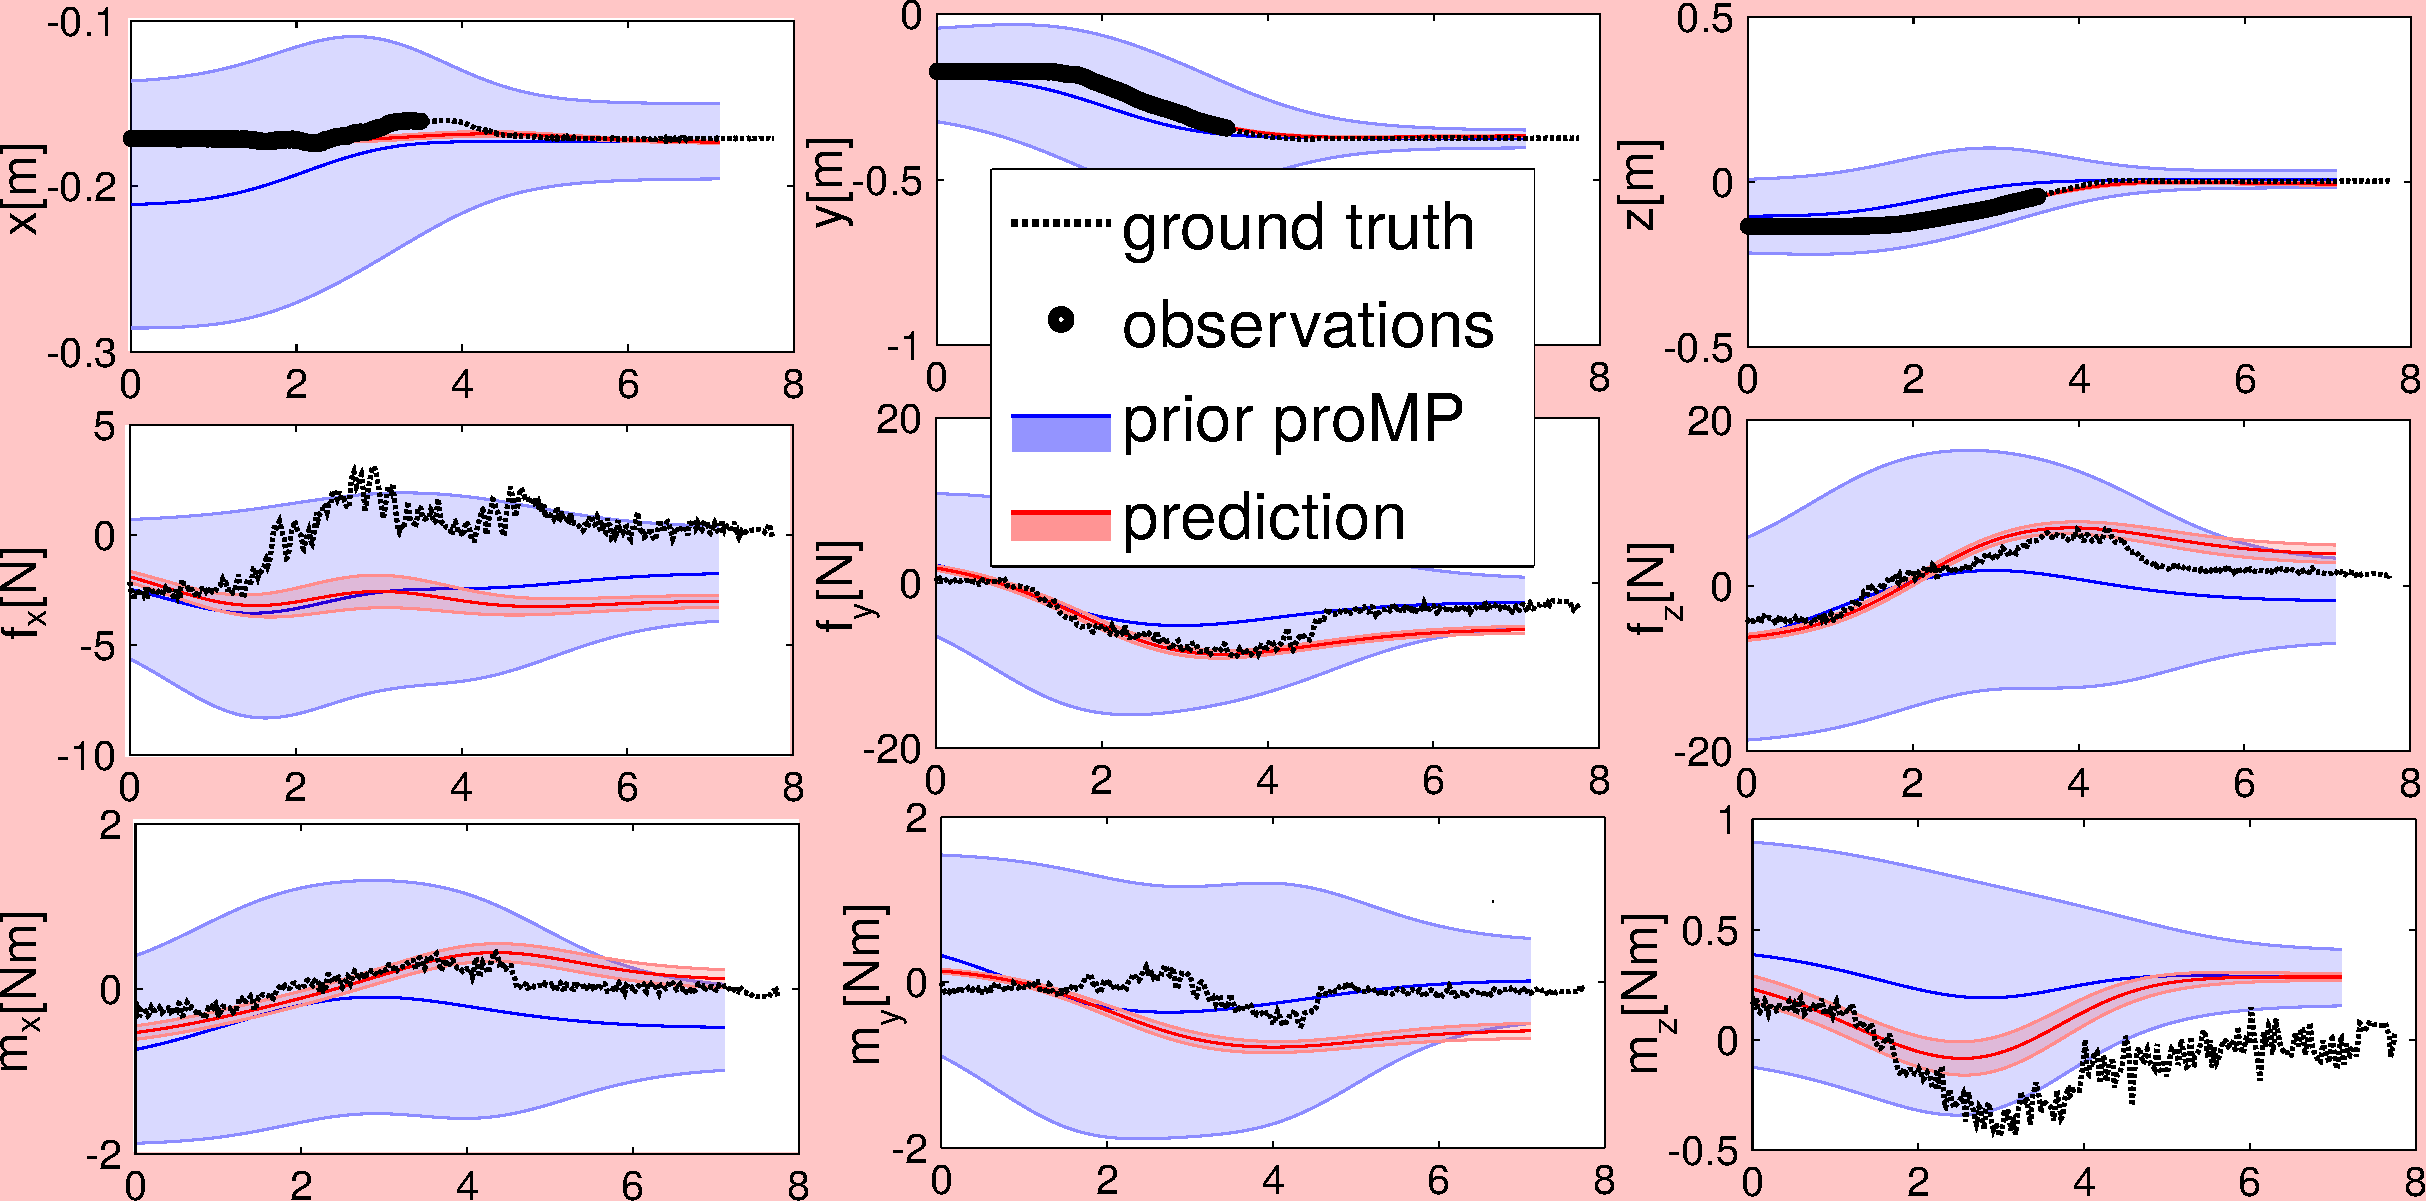
\includegraphics[width=15cm]{img/infA.pdf}\\
%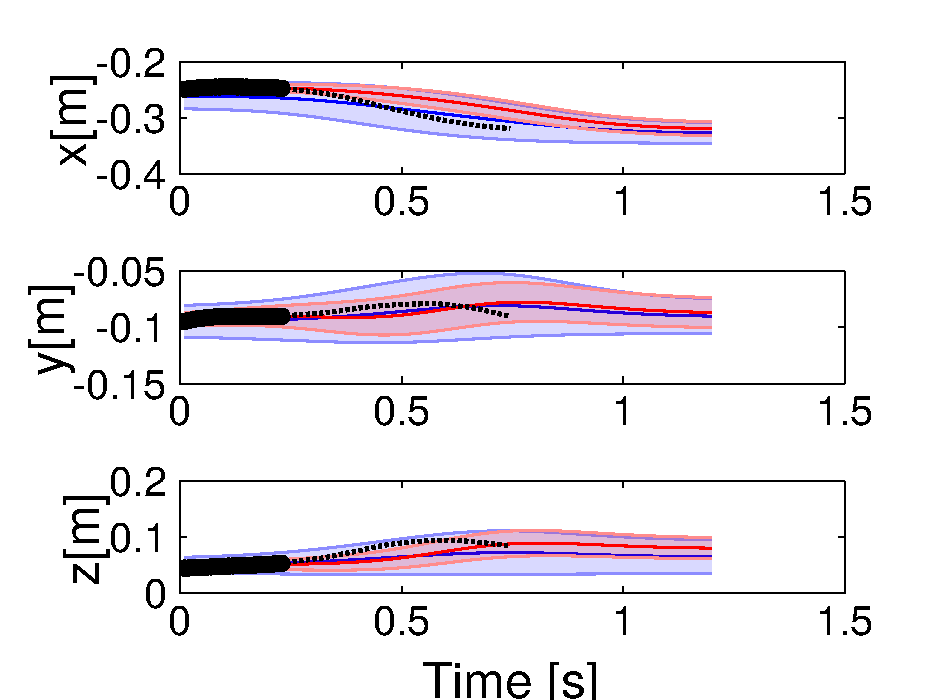
\includegraphics[width=\hsize /3]{img/infData3D/bottom30.pdf}
\textcolor{blue}{B}\\
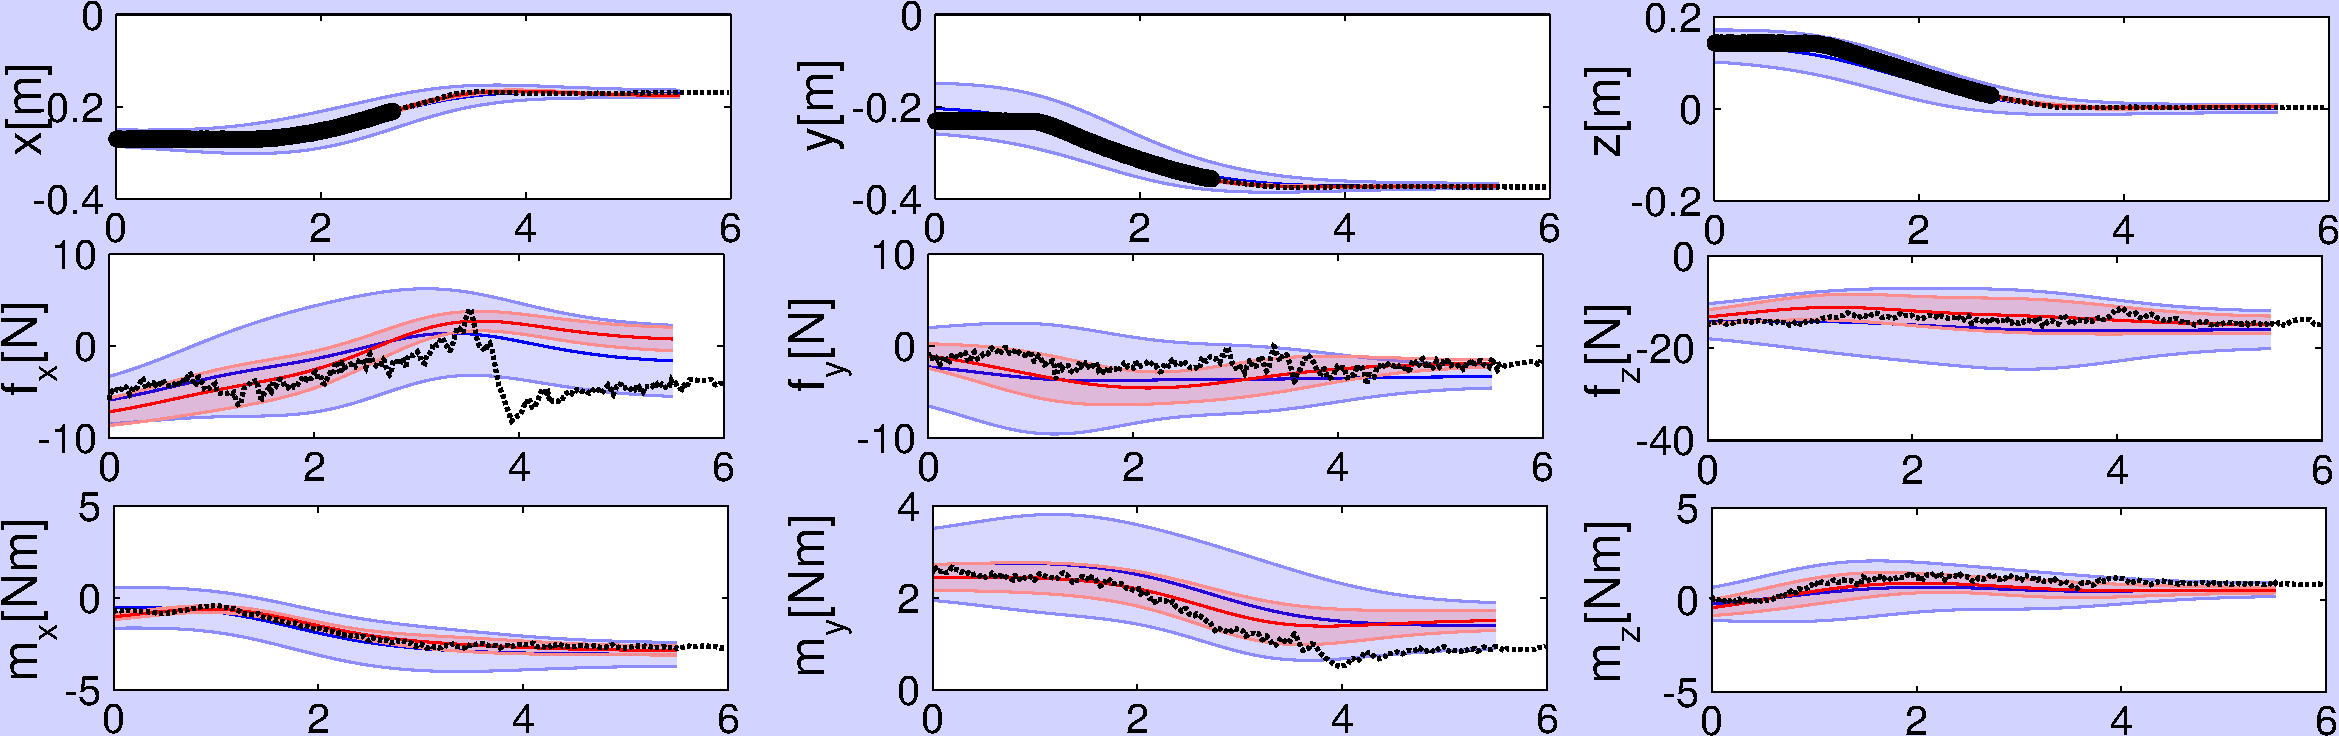
\includegraphics[width=15cm]{img/infb.pdf}\\
%%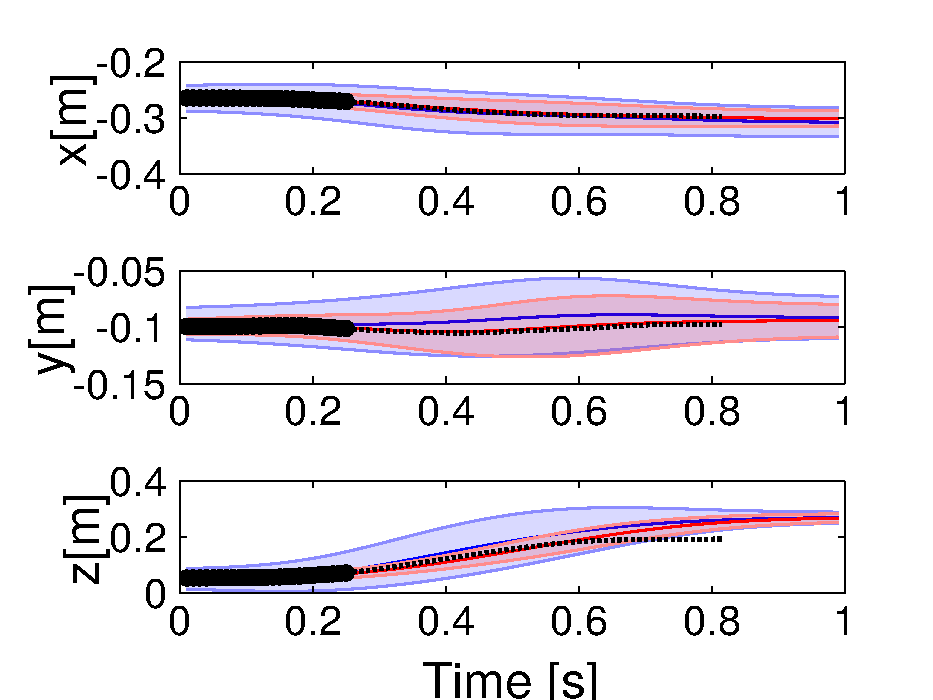
\includegraphics[width=\hsize /3]{img/infData3D/middle30Err.pdf}
\textcolor{green}{C}\\
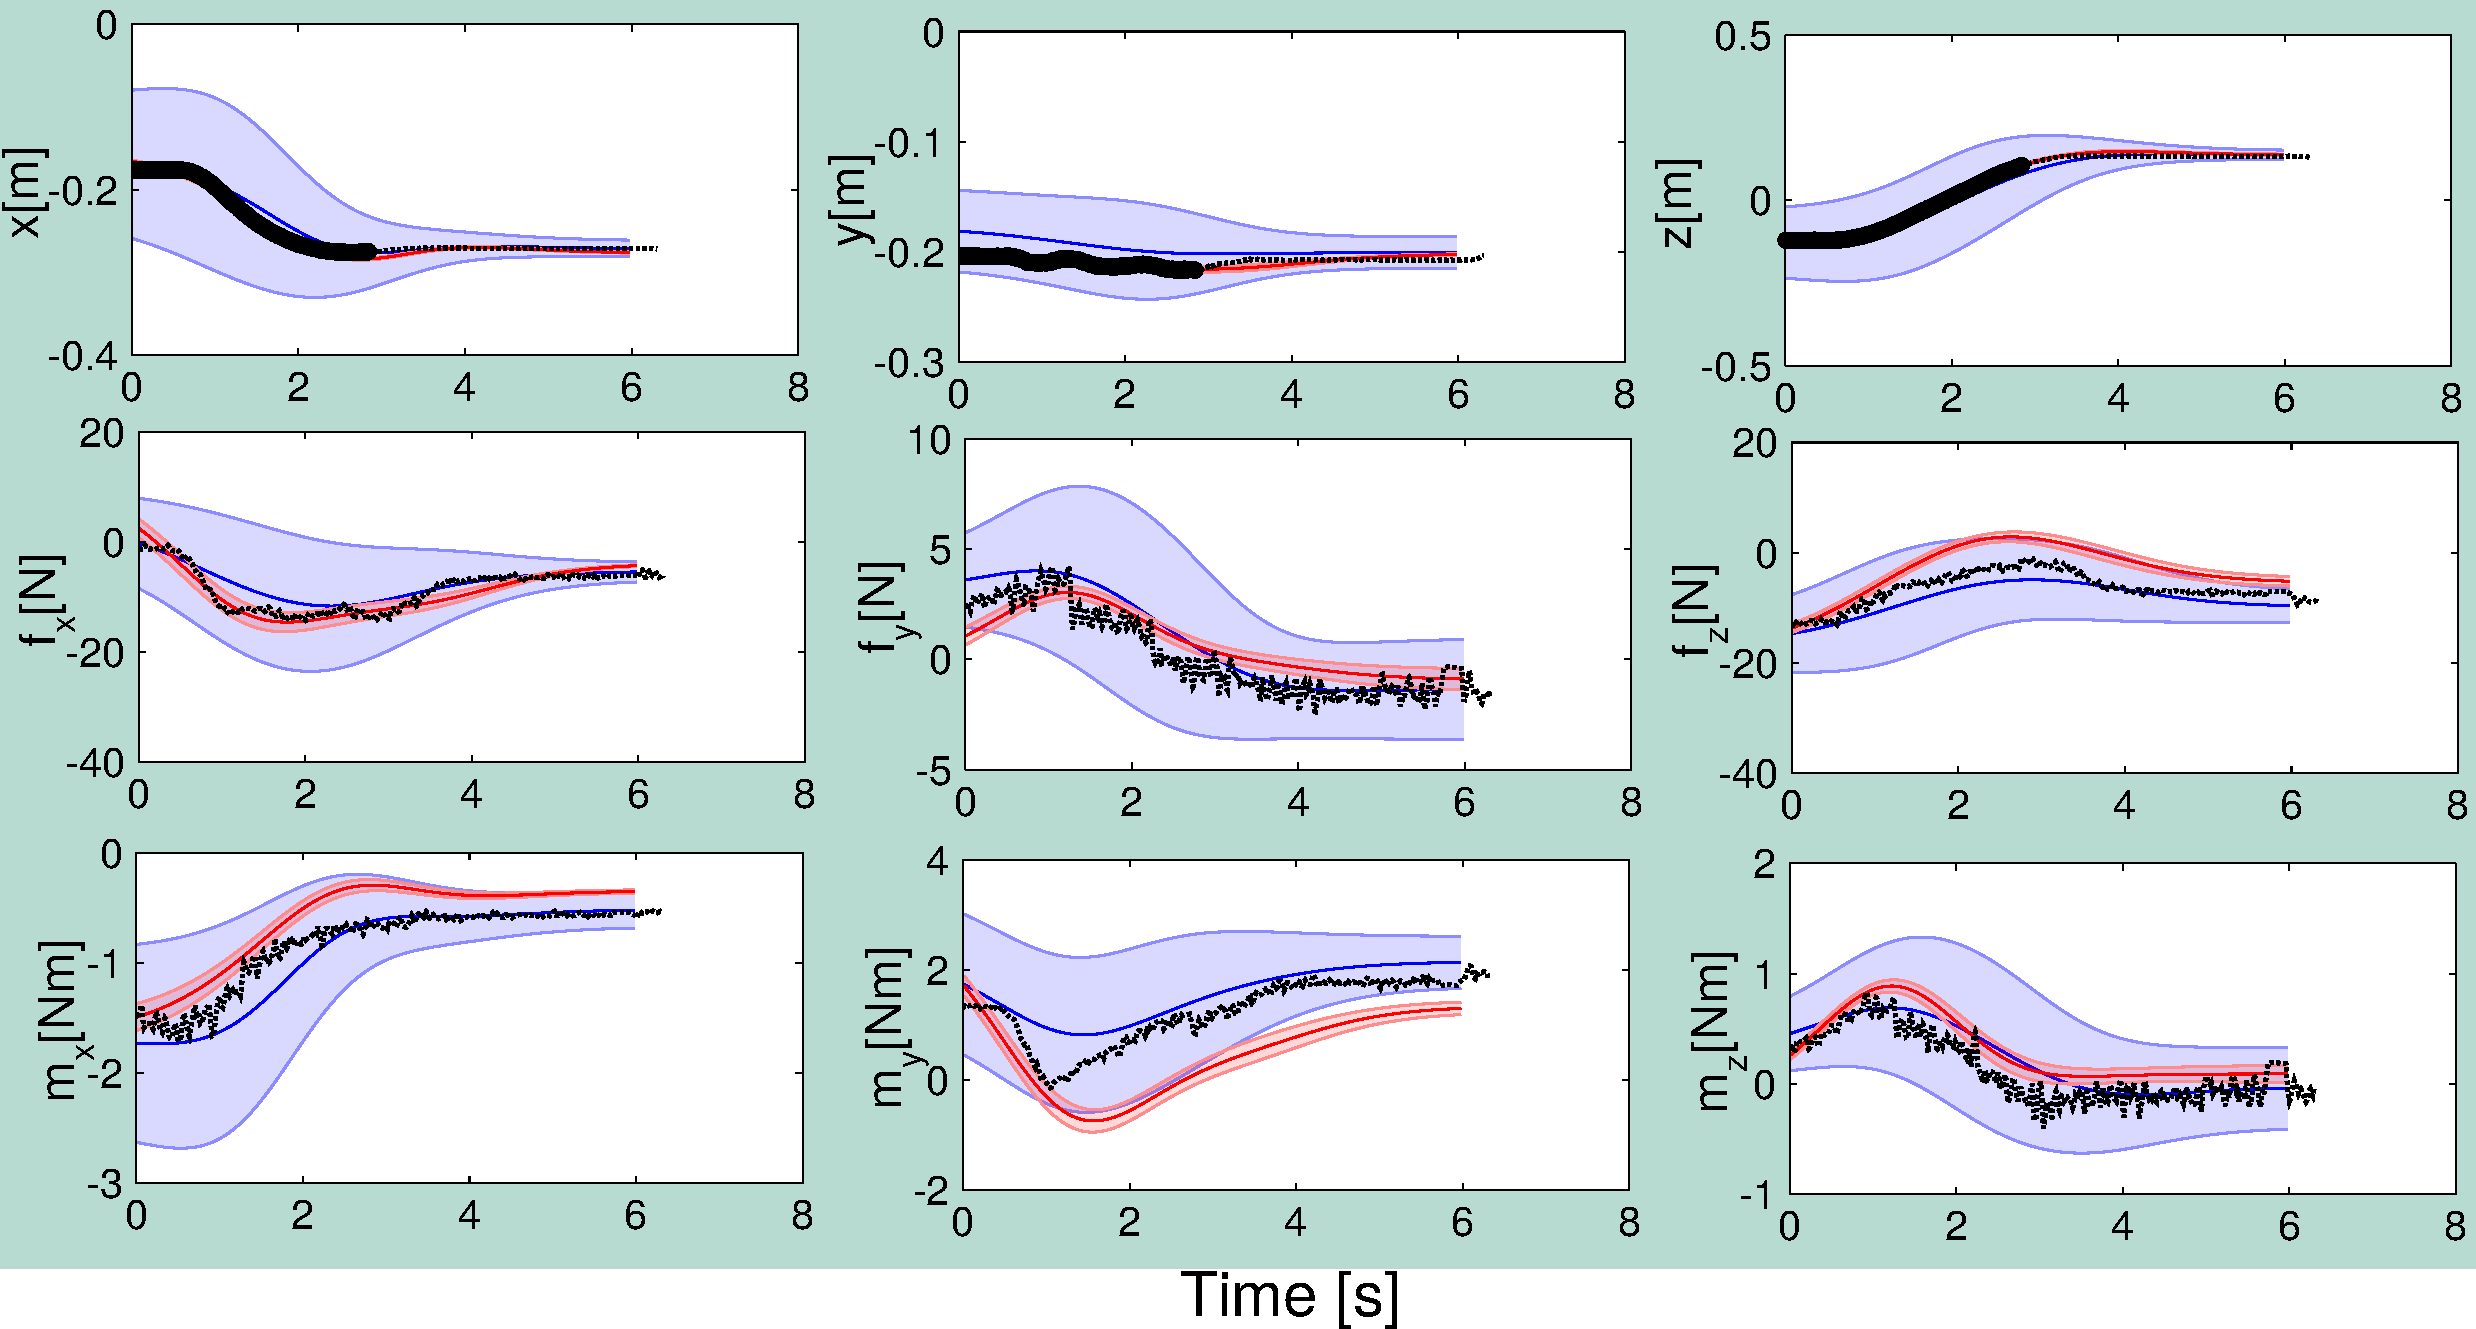
\includegraphics[width=15cm]{img/infc.pdf}\\
%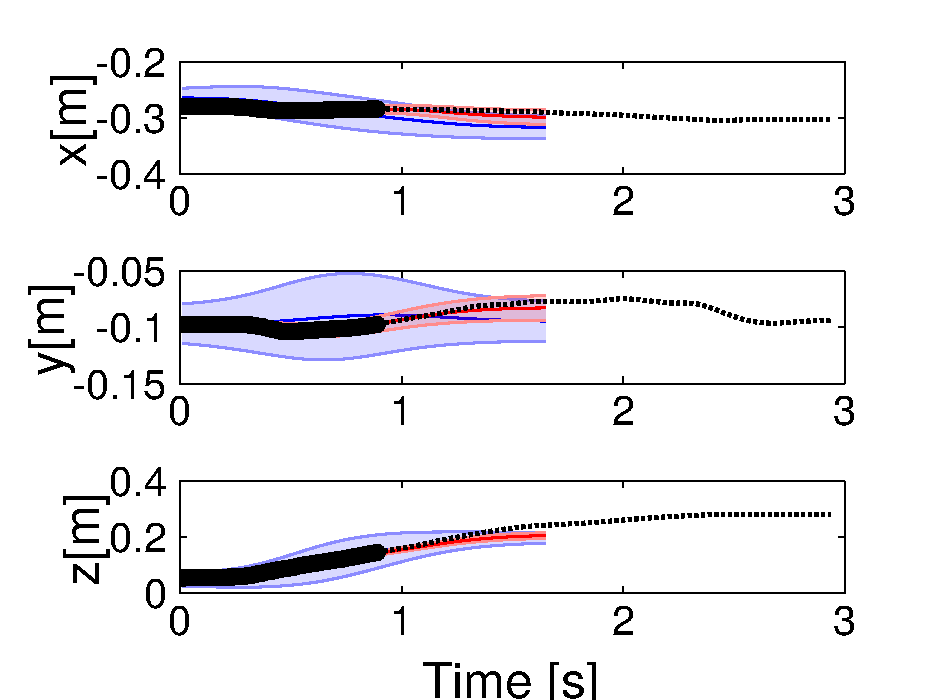
\includegraphics[width=\hsize /3]{img/infData3D/top30.pdf}
}
\caption{Prédiction de la trajectoire future après l'observation partielle ($40\%$) de celle-ci. Cette prédiction est effectuée à l'aide des \textit{ProMPs} définies par leur position Cartésienne. Ces \textit{ProMPs} sont apprises à partir des trois ensembles de trajectoires correspondant aux trois tâches. Ces trajectoires sont effectuées avec le robot \textit{iCub} réel (Figure \ref{fig:realDistribution}).}
\label{fig:realTrajectoriesPredictions}
\end{figure}

Puis, l'inference du but de la trajectoire est effectuée. La Figure~\ref{fig:realTrajectoriesPredictions} représente l'inférence de trois trajectoires testées (chacune correspondant à des tâches différentes) et où l'information des forces et des couples n'est pas utilisée. 
Afin de réaliser cette figure qui compare la trajectoire prédite et la trajectoire attendue, l'algorithme a été ici effectué en hors-ligne. En effet, il n'est pas possible d'avoir de vérité terrain sans avoir récupérée la trajectoire entière en amont. Ainsi, une trajectoire de démonstration a été récupérée de l'ensemble de test (\textit{c.à.d.} qu'elle n'a pas été utilisée pour l'apprentissage) en tant que ``vérité terrain''. Il s'agit alors de la trajectoire attendue.
Dans la Figure~\ref{fig:realTrajectoriesPredictions}, la vérité terrain est présentée en noir, alors que la portion de trajectoire qui est utilisée lors de l'inférence (\textit{c.à.d} les ``observations initiale'') est représentée par des point plus gros en noir.
%\rev{These tests have been done on a test base, that contains some whole-trajectories guided by the user. Then, we give to the program only a partial trajectory composed on 40\% of the recorded trajectory. The ground truth (\textit{e.g.} the total-trajectories of the test base) are represented in the figure in black. The partial-trajectories, that are known by the software are represented with the black circles.} 
Cette figure met en évidence que l'inférence de la position Cartésienne est correcte, malgré qu'une erreur d'une seconde est visible sur l'estimation de la durée de la trajectoire inférée pour la tâche A. De plus, l'inférence des forces et des couple n'est pas très précise. Cela est possiblement dû au fait que la variation des forces et des couples n'est pas corrélée à la variation positionnelle, or le robot prédit la trajectoire en utilisant l'information de la position seule, sans l'information provenant des forces et des couples.
Afin d'améliorer ce résultat, il faut alors ajouter la connaissance des mesures des forces et des couples lors de l'inférence, comme présenté dans la Figure~\ref{fig:realTrajectoriesPredictionsWithForces}. Cette figure montre que l'estimation de la durée des trajectoire est plus précise. Le désavantage est par contre que la position Cartésienne inférée est un peu moins précise, puisque la distribution de la \textit{ProMP} est mise à jour en faisant un compromis entre les mesures de la position Cartésienne et celle des forces et des couples. De plus, afin de permettre une prédiction correcte des forces et des moments, l'estimation du bruit doit être augmenté dans ces dimensions. Ainsi, dans de futures versions, il s'agira d'ajouter la possibilité de faire varier les modèles de bruit selon les trajectoires observées (\textit{c.à.d} que l'on aura  $\Sigma_\Xi^o = \left[
\begin{array}{c c}
\Sigma_X  & 0\\  
0 &\Sigma_F \\
\end{array}\right]$. Ainsi, la covariance sera plus grande en ce qui concerne les données des forces et des couples, que celle concernant les données positionnelles.)
%allow to have different expectation noises according to the data type
%\textcolor{blue}{expectation noises [Obs.: Is “noise
%expectation” or “expectation noise” the same as “observation noise”?]}
%\textcolor{purple}{@marco: i didn't understand your question but tell me if it is more clear now with the following parenthesis} 

Afin de confirmer ces résultats, nous avons annalysé l'inférence des trajectoire et l'estimation du paramètre $\alpha$, selon différente longueure de trajectoire observée (de $30$ à $90\%$ de la trajectoire totale). Pour chacun de ces pourcentages, $20$ tests ont été effectués, avec ou sans données sur les forces et les moments.

Dans la Figure~\ref{fig:errBoxWithWithoutForces}, chaque graphique représente les erreurs de ces $20$ tests. En haut, le critère d'erreur correspond à la distance moyenne entre la trajectoire prédite et celle réelle. Ce graphe montre que l'inférence de la position Cartésienne de la trajectoire effectuée par la main du robot est plus précise sans prendre en compte l'information des forces et des couples. En bas, le critère d'erreur correspond à la distance moyenne entre l'estimation du paramètre $\alpha$ et sa vrai valeur. Cette fois-ci, les données des forces et des couples permettent d'approximer mieux le paramètre $\alpha$.
Ainsi, ces graphes confirment les hypothèses proposées concernant les Figures~\ref{fig:realTrajectoriesPredictions} et ~\ref{fig:realTrajectoriesPredictionsWithForces}.
\todo{j'ai jamais précisé que c'est logique que l'information des forces permettent de mieu estimer le paramètre alpha ?} 

La médiane, la moyenne et la variance de ces erreurs de prédiction, calculées à l'aide de l'erreur quadratique moyenne (\textit{NRMSE}), sont reportés dans la Table~\ref{table:statsError}. 
\toimprove{L'erreur de prédiction du paramètre de modulation du temps correspond à un scalaire} : $|\alpha_{\textrm{prediction}} - \alpha_{\textrm{real}} |$.   
L'erreur de prédiction de la trajectoire est calculée à l'aide du \textit{NRMSE} de $| \Xi_{\textrm{prediction}} - \Xi_{\textrm{real}}  |$.

Dans l'étude suivante, nous utiliserons alors l'information des couples et des forces uniquement lors de l'estimation du paramètre de modulation du temps $\alpha$. Cela permettra d'avoir à la fois la meilleur inférence de la trajectoire estimée , mais aussi la meilleur estimation du paramètre de modulation du temps. Ainsi l'algorithme combinera les benéfice de prédiction effectuée avec ou sans l'information des forces et des moments.

La Table~\ref{table:statsError} reporte aussi le temps moyen de calcul nécessaire à la prédiction du paramètre de modulation du temps et de la distribution postérieure. Les calculs sont effectués sur Matlab, sur un ordinateur à un cœur  (\textit{e.g.} sans parallélisation). Alors que le temps de calcul dans le cas de calcul ``sans forces et moments'' est correcte pour des applications en temps réel, en utilisant l'information des forces et des moments, la prédiction est plus lente ce qui limite l'utilisation en temps-réel de cette application lorsque des décisions rapides doivent être prises par le robot.
\todo{C'est pourquoi, dans la troisième étude de cette thèse, nous chercherons à diminuer la dimensionnalité des \textit{ProMPs} lorsque l'on souhaite apprendre les mouvements \toimprove{du corps entier du partenaire du} robot.}
% Computation time will be improved in the future works, with the implementation of the prediction in an iterative way.


%or change the tolerance interval of accepted wrenches \todo{as represented in figure\ref{}}.

\begin{figure}[!h]
\centering
{
\textcolor{red}{A}\\
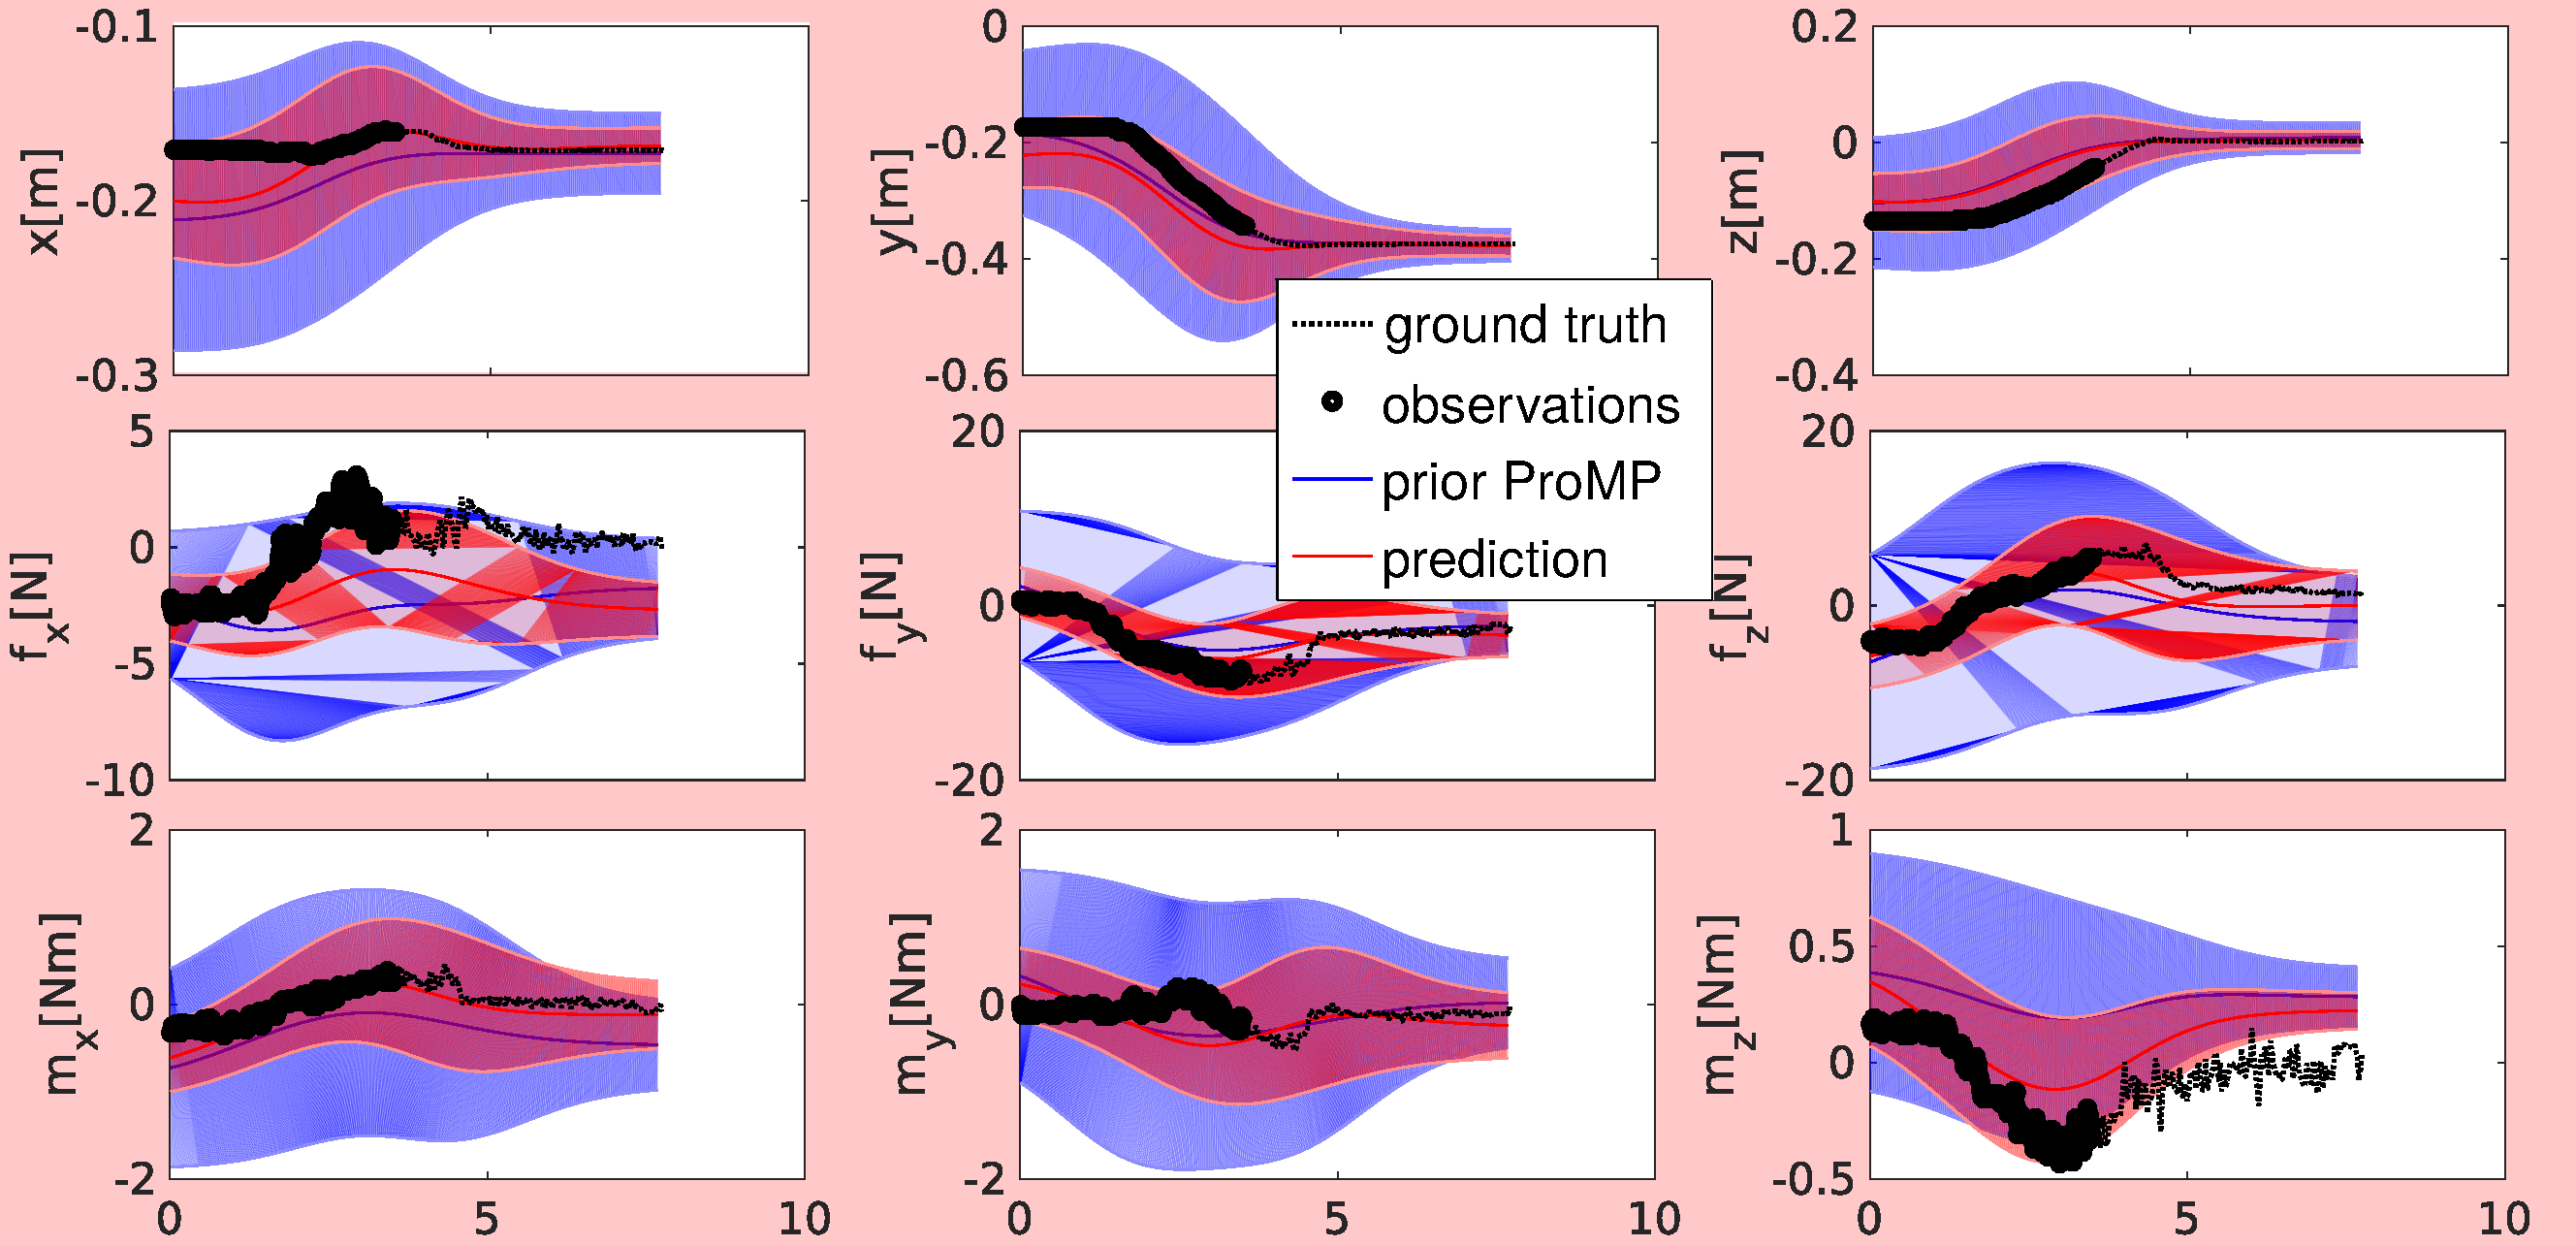
\includegraphics[width=14cm]{img/withWrenchInfA.pdf}\\
\textcolor{blue}{B}\\
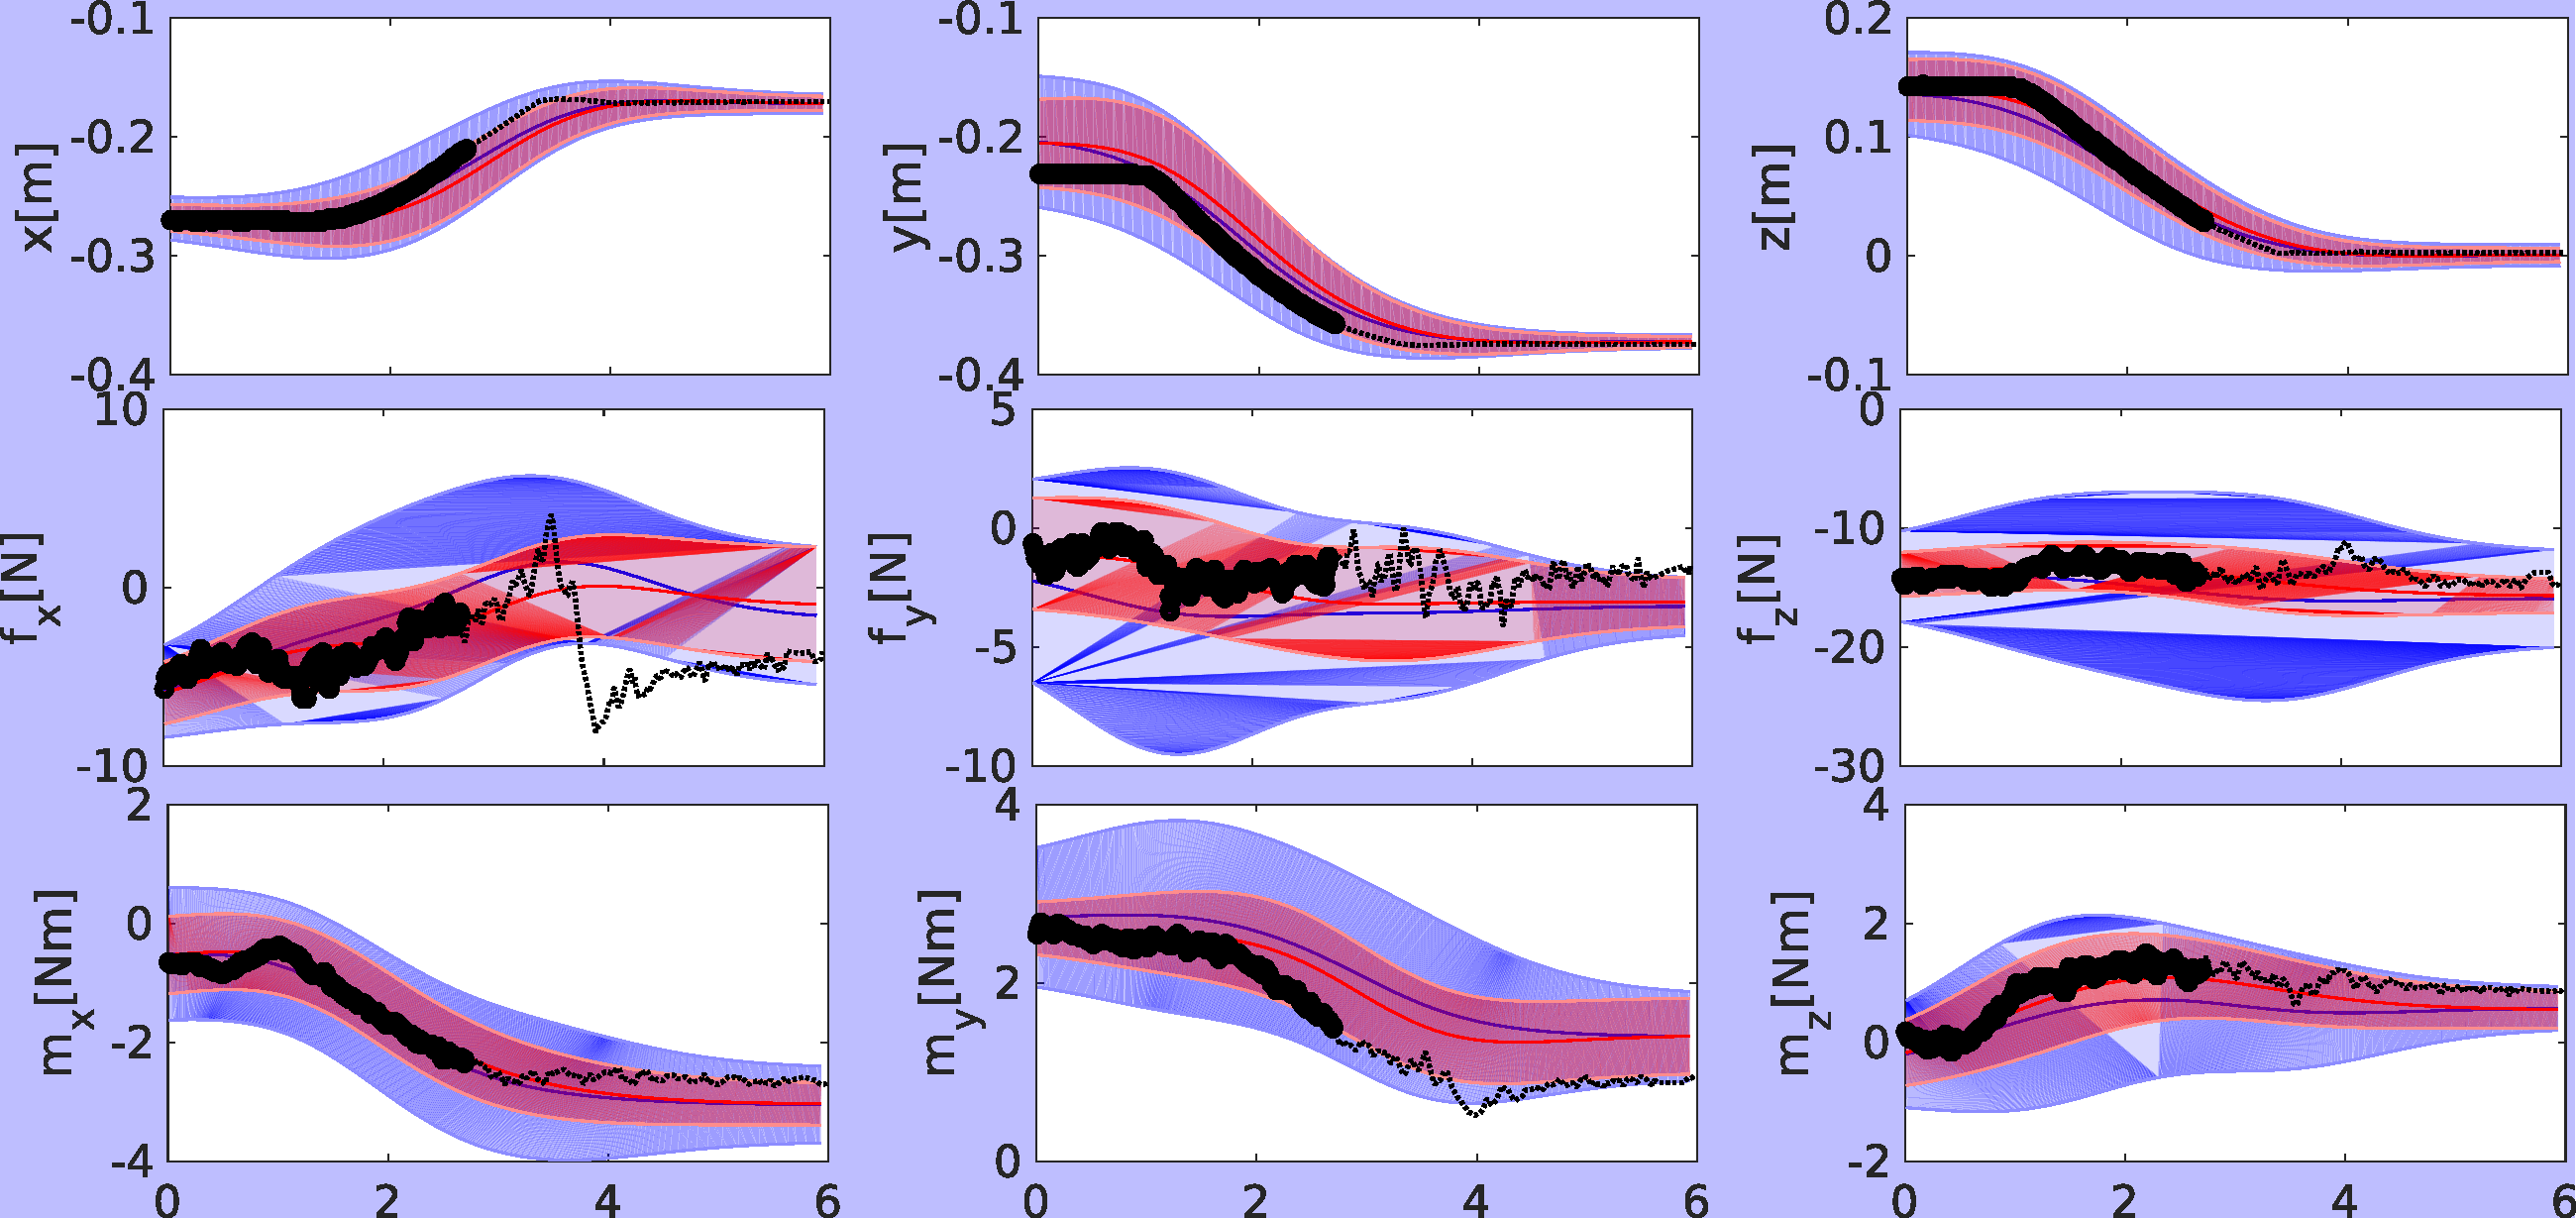
\includegraphics[width=14cm]{img/withWrenchInfB.pdf}\\
\textcolor{green}{C}\\
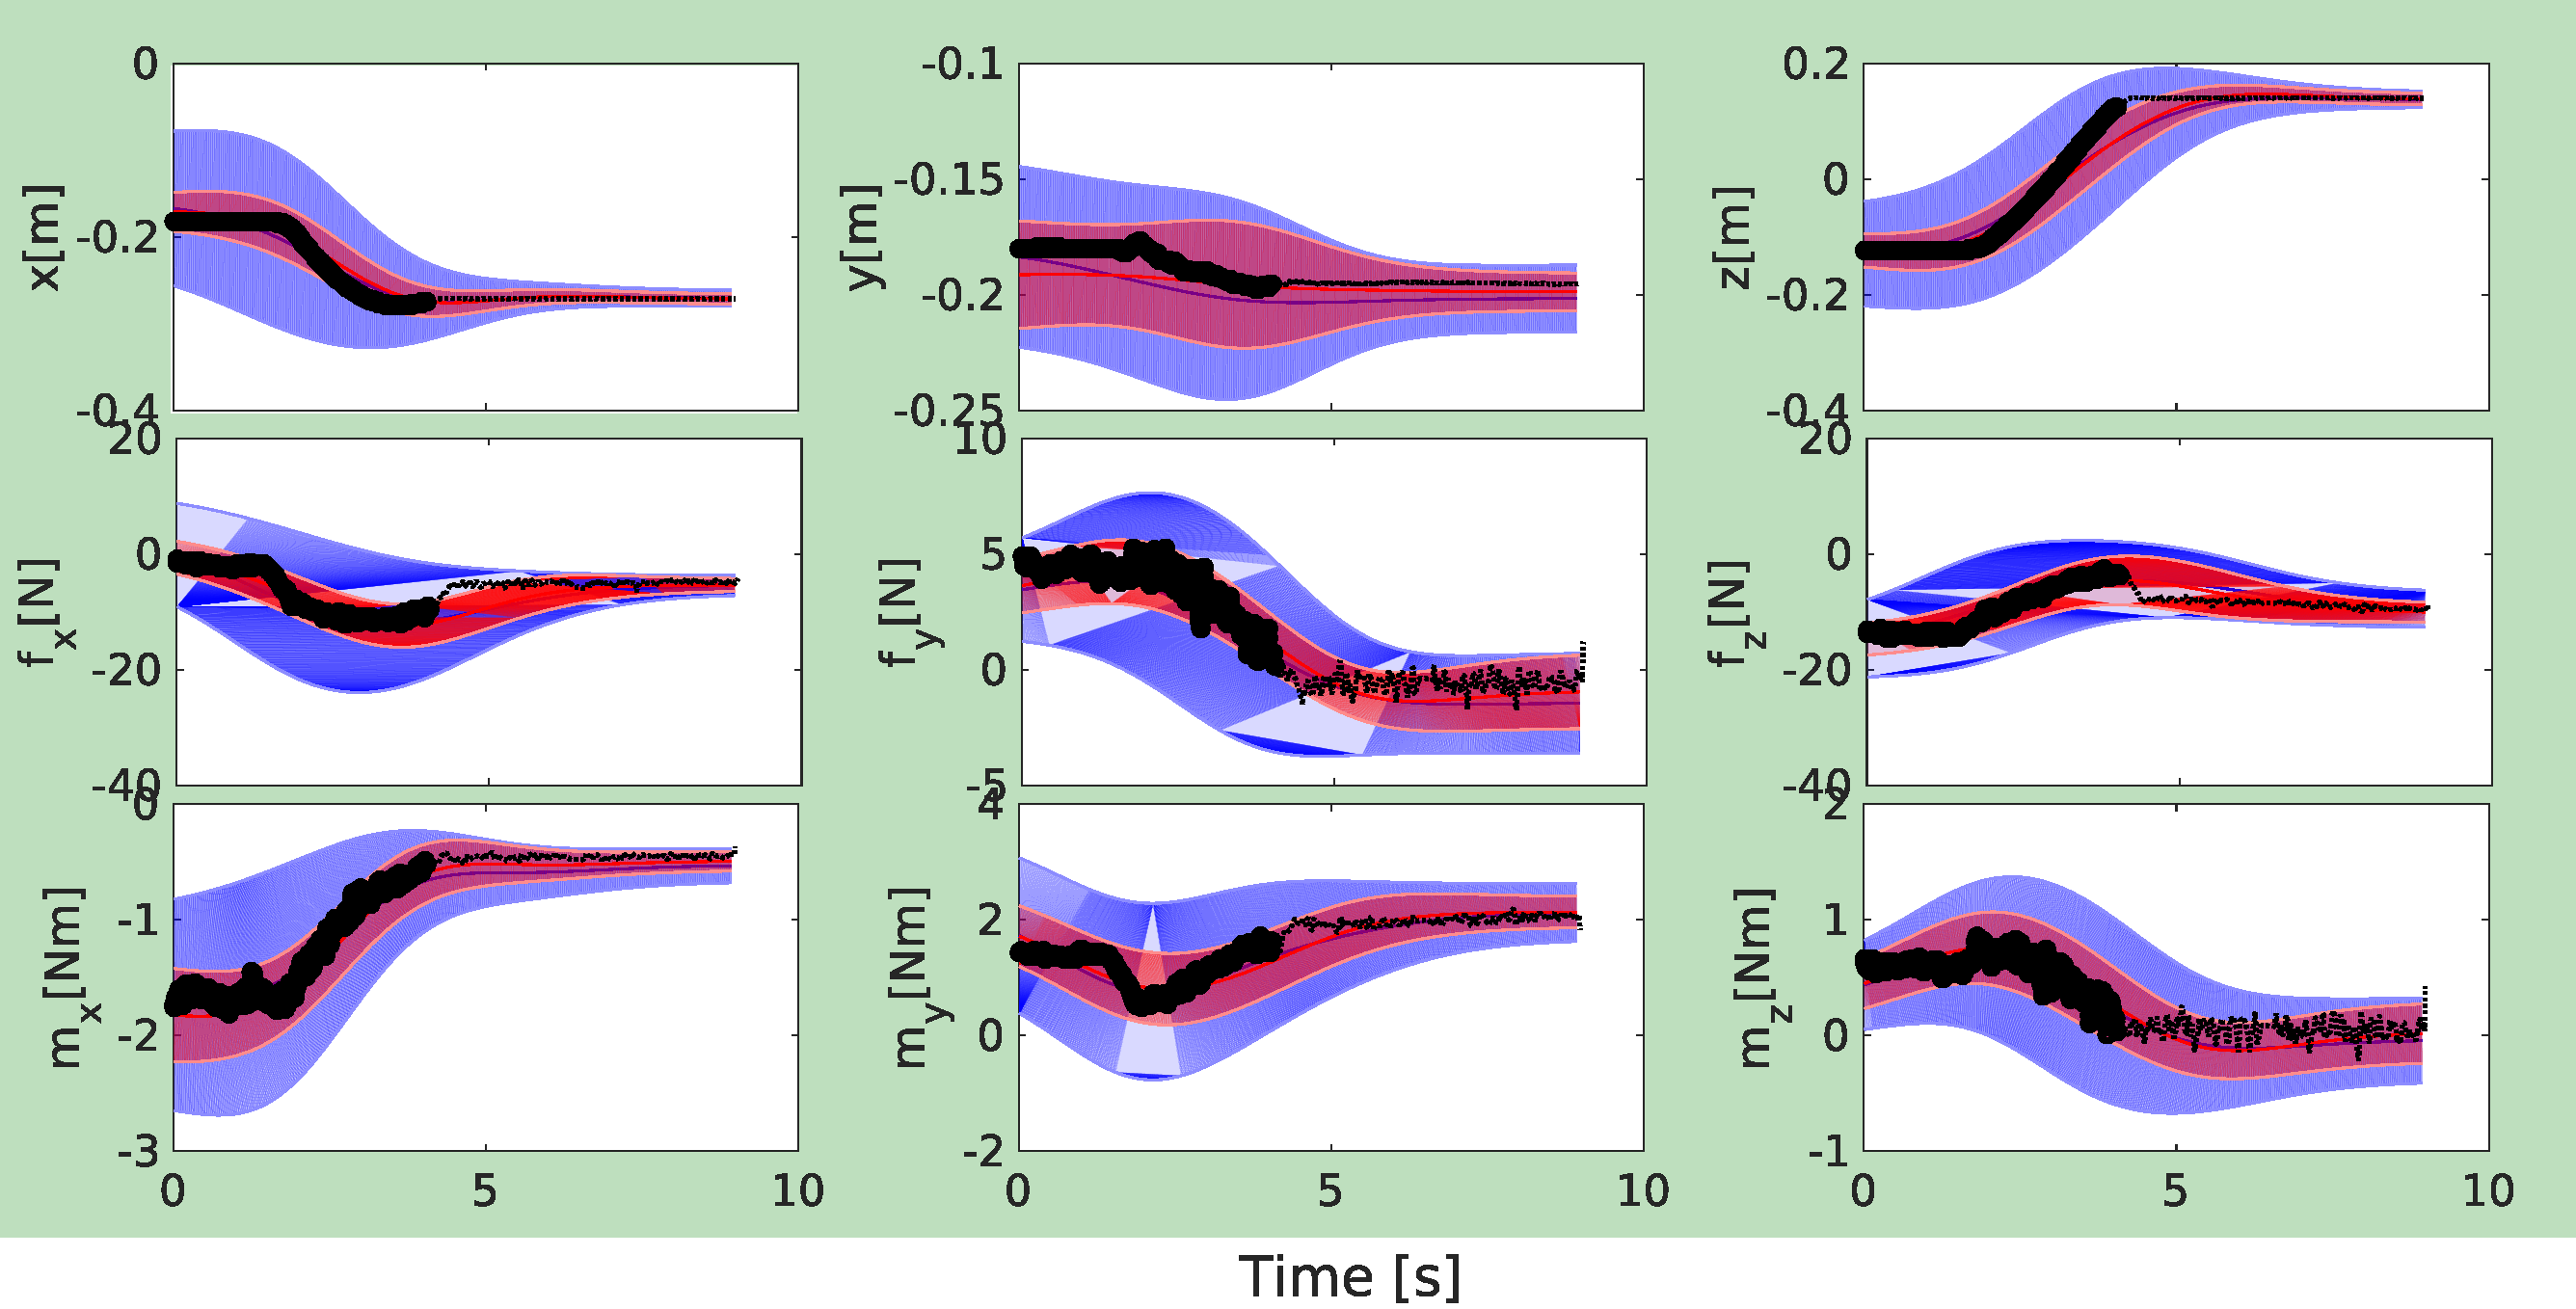
\includegraphics[width=14cm]{img/withWrenchInfC.pdf}\\
%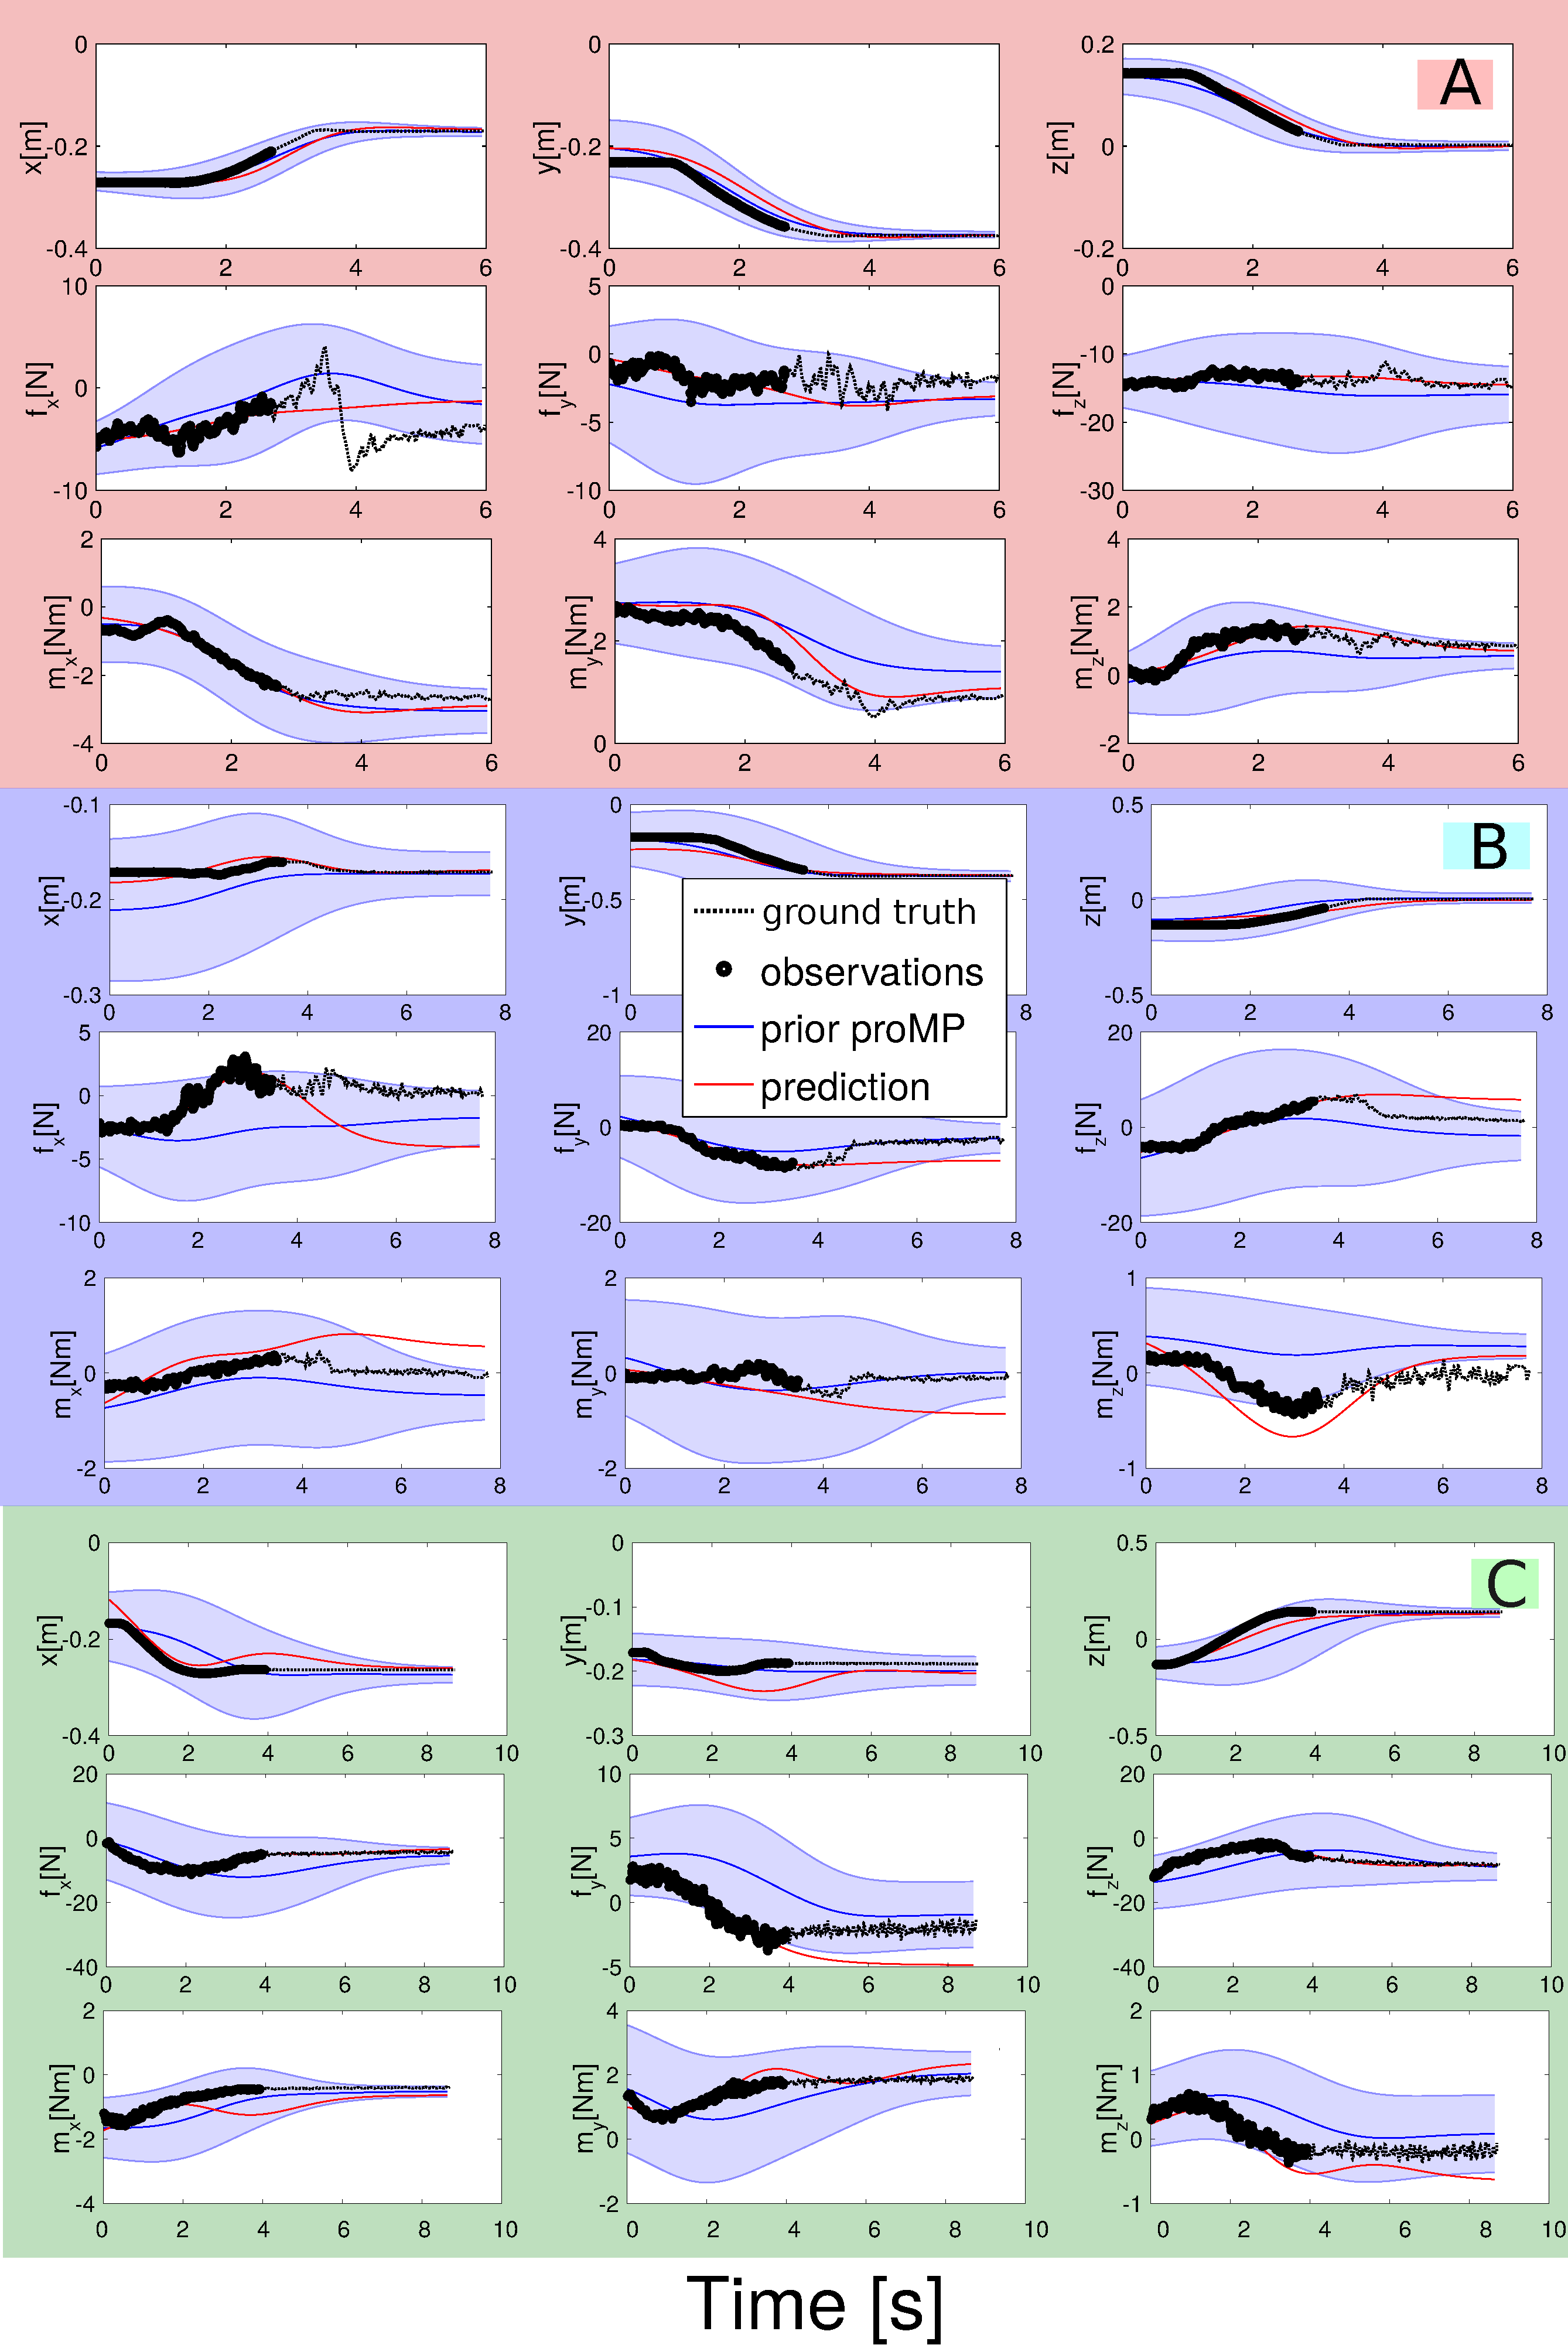
\includegraphics[height=20cm]{img/infUseForces.pdf}
}
\caption{
Prédiction de la trajectoire future après l'observation partielle ($40\%$) de celle-ci. Cette prédiction est effectuée à l'aide des \textit{ProMPs} définies par leur position Cartésienne et les forces et moments externes. Ces \textit{ProMPs} sont apprises à partir des trois ensembles de trajectoires correspondant aux trois tâches. Ces trajectoires sont effectuées avec le robot \textit{iCub} réel (Figure \ref{fig:realDistribution}).}
\label{fig:realTrajectoriesPredictionsWithForces}
\end{figure}


\begin{figure}[!h]
\centering
{
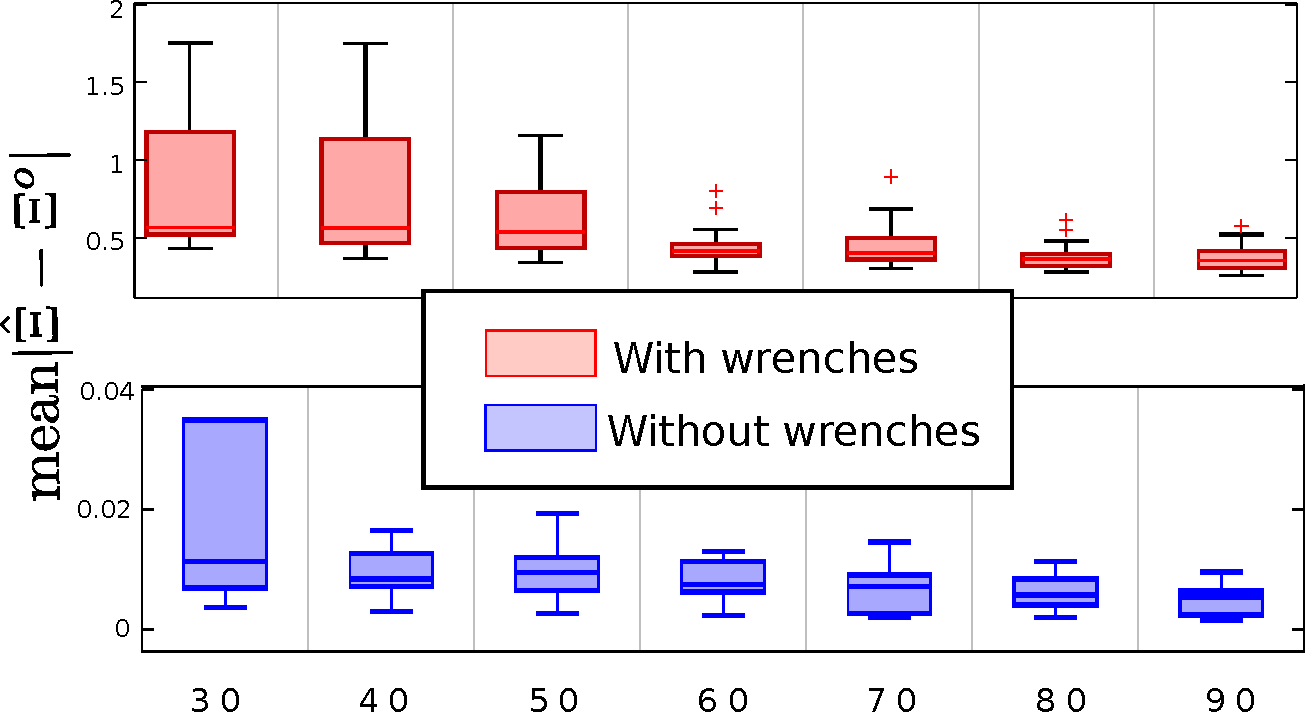
\includegraphics[width=12cm]{img/errBoxWithWithoutForces.pdf}\\
\includegraphics[width=12cm]{img/boxAlphaErrorWithForces.pdf}
}
\caption{Erreur de prédiction de la trajectoire (en haut) et erreur d'estimation du paramètre de modulation du temps (en bas) de la trajectoire inférée avec ou sans l'information des forces et des couples, pour les ensembles de trajectoires correspondant aux trois tâches, trajectoires effectuées sur le robot \textit{iCub} réel (\textit{c.f.} Figure~\ref{fig:realDistribution}).}
\label{fig:errBoxWithWithoutForces}
\end{figure}

%\begin{table}
%\centering
%\begin{tabular}{|c|c|c|c|c|c|c|c|}
% \hline
% Percentage of observations & 30 & 40 & 50 & 60 & 70 & 80 & 90 \\
% \hline
% Trajectory prediction error &   &    &    &    &    &    &    \\
% \hline
% Time modulation prediction error & & & & & & & \\
% \hline
% Computation time for prediction & & & & & & & \\
% \hline
%\end{tabular}
%\caption{ \todo{ORIANE FILL IT}}
%\label{table:statsError}
%\end{table}

\begin{table}
\begin{center}
\textbf{Avec les forces et moment}
\begin{tabular}{|p{3.6cm}|p{2cm}|c|c|c|c|}
  \hline 
   \% de la trajectoire observée ($\simeq$ nb. d'échantillons) &  & \textbf{$30 (\simeq 180$)} & \textbf{$50 (\simeq 300$)} & \textbf{$70 (\simeq 419$)} & \textbf{$90 (\simeq 539$)}  \tabularnewline
  \hline
\multirow{3}{3cm}{Erreur de prédiction du paramètre $\alpha$} &  médiane & 2.26e-08 & 1.35e-08 & 3.61e-09 & 8.95e-09 \tabularnewline
 % \hline
  \cline{2-6} & moyenne & 4.26e-02 & 7.81e-09 & 2.19e-08 & 2.09e-08 \tabularnewline
 \cline{2-6} & variance & 1.08e-02 & 1.09e-16 & 5.44e-16 & 2.24e-16 \tabularnewline
  \hline
\multirow{3}{3cm}{Err. de prédiction de la trajectoire (NRMSE) [m]} &  médiane & 2.73e-01 & 5.51e-01 & 4.52e-01 & 5.38e-01 \tabularnewline
 % \hline
  \cline{2-6} & moyenne & 8.11e-01 & 5.86e-01 & 5.29e-01 & 3.42e-01 \tabularnewline
 \cline{2-6} & variance & 7.45e-01 & 1.36e-01 & 7.74e-02 & 2.93e-02 \tabularnewline
  \hline  
\multirow{2}{3cm}{Temps de calcul [s]} &  moyenne & 0.25 & 0.74 & 1.92 & 3.59 \tabularnewline
 \cline{2-6} & variance & 0.01 & 0.27 & 2.77 & 4.81 \tabularnewline
 \hline
\end{tabular}

\vspace{0.4cm}
\textbf{Sans forces et couples}
\begin{tabular}{|p{3.6cm}|p{2cm}|c|c|c|c|}
  \hline 
   de la trajectoire observée ($\simeq$ nb. d'échantillons) &  & \textbf{$30 (\simeq 180$)} & \textbf{$50 (\simeq 300$)} & \textbf{$70 (\simeq 419$)} & \textbf{$90 (\simeq 539$)}  \tabularnewline
  \hline
\multirow{3}{3cm}{Erreur de prédiction du paramètre $\alpha$} &  médiane & 1.19e-02 & 1.76e-02 & 1.74e-02 & 1.62e-02 \tabularnewline
  \cline{2-6} & moyenne & 2.81e-02 & 1.92e-02 & 2.45e-02 & 1.43e-02 \tabularnewline
 \cline{2-6} & variance & 9.51e-04 & 1.00e-04 & 3.37e-04 & 1.82e-04 \tabularnewline
  \hline
\multirow{3}{3cm}{Err. de prédiction de la trajectoire (NRMSE) [m]} & médiane & 4.53e-02 & 4.73e-02 & 7.20e-02 & 6.20e-02 \tabularnewline
 % \hline
  \cline{2-6} & moyenne & 1.56e-01 & 7.36e-02 & 5.75e-02 & 4.29e-02 \tabularnewline
 \cline{2-6} & variance & 5.04e-02 & 1.80e-03 & 1.80e-03 & 6.0e-04 \tabularnewline
  \hline  
\multirow{2}{3cm}{Temps de calcul [s]} &  moyenne & 6.89e-02 & 8.49e-02 & 1.43e-01 & 2.58e-01 \tabularnewline
 \cline{2-6} & variance & 2.83e-03 & 1.19e-03 & 7.31e-03 & 2.45e-03 \tabularnewline
 \hline
\end{tabular}
\end{center}
\caption{Moyenne et variance \todo{(ou écart type?)} du \textit{NRMSE} des erreurs de prédiction affichées dans la Figure~\ref{fig:errBoxWithWithoutForces}, et moyenne des temps de calcul nécessaires aux prédictions (\textit{c.à.d.} prédiction du paramètre $\alpha$ et de la trajectoire). Les calculs sont effectués sous Matlab, avec un ordinateur à un cœur (\textit{e.g.} sans parallélisation).}
\normalcolor
\label{table:statsError}
\end{table}


\begin{figure}[ht]
\centering
\includegraphics[width=0.5\hsize]{img/realXp.pdf}
\caption{\rev{Seconde expérience avec le robot : \textit{iCub} doit trier les objets dans deux corbeilles, grâce à un guidage partiel de l'utilisateur. Si l'objet est correct, le robot doit déplacer l'objet dans la corbeille placée devant lui, sinon dans la corbeille à sa gauche. Les mouvements permettant de mettre les objets dans ces corbeilles sont différents. Afin de simplifier, les endroits où le robot doit lâcher les objets dans les corbeilles sont représentés ici par ``F'' et ``L''. Après avoir inspecté l'objet, l'utilisateur guide partiellement le robot vers la gauche ou la droite.}}
\label{figure:sortingiCub}
\end{figure}

\begin{figure}[ht]
\centering
\textbf{Action dirigée vers l'avant (F)}\\
\includegraphics[width=0.8\hsize]{img/FRONT2modif.pdf}\\
\textbf{Action dirigée vers la gauche (L)}\\
\includegraphics[width=0.8\hsize]{img/FigLeft.pdf}
\caption{Trajectoires prédites pour la seconde expérience avec le robot (Figure \ref{figure:sortingiCub}). Les gros points noirs représentent les observations du robot lorsque son utilisateur guide physiquement son bras. Lorsque le partenaire lâche le bras du robot, celui-ci prédit la trajectoire future et la continue. La distribution à priori de la \textit{ProMP} reconnue est présentée en bleu; la distribution postérieur de cette \textit{ProMP}, utilisée pour effectuer la trajectoire prédite est présentée en rouge ; la \textit{ProMP} de l'autre tâche est présentée en vert. \textbf{En haut, F} : l'utilisateur déplace le bras du robot vers la corbeille placée en avant. Après $0.5$seconde, le robot reconnaît que le mouvement correspond à l'action ``F''. \textbf{En bas, L} : l'utilisateur déplace le bras du robot vers la corbeille placée à la gauche du robot. Après environ $0.25$ seconde, le robot reconnaît l'action``L''.}
\label{figure:sortingiCubTrajectories}
\end{figure}


\subsection{Tri collaboratif d'objets}

\toimprove{La seconde expérience réalisée avec le \textit{iCub} réel, a été présentée au début de la Section~\ref{sec:appliRealIcub} où celui-ci doit trier des objets dans deux corbeilles (\textit{c.f.} Figure~\ref{figure:sortingiCub}) à l'aide de deux primitives de mouvements, l'une en direction de la corbeille placée à sa gauche, et l'autre pour celle placée devant lui. Le robot doit lâcher l'objet à différentes hauteurs, avec différents gestes de la main et différentes orientations de celle-ci}. \todo{repetion}
C'est pourquoi, la modélisation de la \textit{ProMP} prend cette fois ci en compte la position Cartésienne de la main $X_t=[x_t,y_t,z_t] \in R^3$ et son orientation $A_t \in R^4$, exprimé en quaternion :
$$\xi_t = \begin{bmatrix} X_t \\ A_t\end{bmatrix} = \Phi_{\alpha t} \, \boldsymbol{\omega} + \epsilon_t$$
Tout comme pour l'expérience précédente, le robot apprend d'abord les primitives par apprentissage kinesthésique (\textit{c.à.d.} que l'on guide physiquement le robot pour que celui-ci apprenne les trajectoires effectuées ), avec une douzaine de démonstrations. Après cette phase d'apprentissage, l'utilisateur peut attraper la main du robot, commencer un mouvement en direction d'une des corbeilles, puis la lâche au moment où l'utilisateur désire que le robot finisse par lui même le mouvement. L'information de  contact sur la peau du robot est utilisée deux fois. Premièrement, quand l'utilisateur attrape le bras, le robot détecte le contact sur sa peau, ce qui lui fait comprendre que la trajectoire est commencée.  Deuxièmement, lorsque le partenaire lâche la main du robot, le robot détecte la fin du contact sur sa peau, ce qui lui fait comprendre que la trajectoire initiée par le partenaire est finie. 
En utilisant cette première portion de trajectoire, le robot reconnaît alors la tâche initiée, et prédit la finalisation du mouvement qui est attendue par le partenaire, puis L’exécute de manière autonome. 
\toimprove{Dans une des vidéos présentée dans la Section~\ref{sec:video}, une pause artificielle est introduite après que l'utilisateur ait initié le mouvement, afin que celui-ci ``valide'' la trajectoire prédite par le robot, à partir de la visualisation de cette trajectoire sur l'interface iCubGui \todo{déjà dit avant}}. 
%The predicted trajectory is shown on the iCubGui.
La Figure~\ref{figure:sortingiCubTrajectories} représente une de ces prédiction effectuée par le robot réel après que l'utilisateur ait relâché la main du robot. Dans cette figure, il n'y a plus de trajectoire représentant la ``vérité terrain'', puisque cette information est inconnue. Cependant, il s'agit de la bonne trajectoire attendu par l'utilisateur.

%\subsection{Model specification}
%\label{modelSpe}
%\todo{I thinks this part is not usefull, isn't it?}
%
%\subsection{Detection of the human intent from contact forces}
%\label{subsec:forces}
%\towrite{Explanation of how the robot's behaviour changes according to the contact force information (master/slave behaviour).}% Idea: We have learned a forces distribution   if$ abs(\tau_ext)$}
%
%Moreover, using the inferred external forces $\hat{F} =[\hat{F}_{n_o+1}, \ldots, \hat{F}_{\hat{t}_{f}}]^\top$, it will changes its behaviour if the users' forces are stronger than the ones it learned (e.g., if $F_t > \hat{F}_t + 1.95 \sqrt{\hat{\sigma}_{\hat{F}_t}}$, 97.5 percentile of the normal distribution)\\
%
%%%%%%%%%%%%%%%%%%%%%%%%%%%%%%%%%%%%%%%%%%%%%%%%%%%%%%%%%%%%%%
%
%
%\subsection{Dynamics and Robot control}
%\towrite{Explanation of the dynamics computation and the robot's movement control in the toy problem (see \ref{toyPblm})}
%\towrite{Explanation of the iCub's software we use to receive forces/ to move the robot, etc.)}
%
%
%\newpage
%%%%%%%%%%%%%%%%%%%%%%%%%%%%%%%%%%%%%%%%%%%%%%%%%%%%%%%%%%%%%%%%%%%%%%%%%%%%%%%%
%\section{Experiments}
%\todo{This part has to be deleted, right?}
%
%\subsection{Moving a simple 2DOF arm}
%\label{toyPblm}
%%Toy problem: I am currently creating a simple 2DOF arm on Matlab (without iCub) in 2D.\\
%%I will add a second arm (human's simulation) to move the first robot arm: I will learn:
%%\begin{itemize}
%%\item The end-effector Cartesian position $X=(x,y,0,0,0\boldsymbol{\omega}_z)^\top$
%%\item The external forces  $F_{ext}= (F_x,F_y,0,0,0,\mu_z)^\top$
%%\end{itemize}
%%This first experiment will present simple figures to explain the problem and how it works. We will present how the robot learns, how it recognizes an initiated movement, how it finishes this recognize movement and how it can stop its  movement when its user wants it to follow him (using force information).\\
%%These figures will complete the methods part and to show that the software works.
%
%\subsection{Moving the simulated iCub arm and predicting the expected task}
%\label{exp:sim}
%Here we will present the real experiment on the simulation. After having recognize and finish the movement, the desired task linked to the movement will be done. (pull/push movement).
%
%\subsection{Moving the real iCub}
%\towrite{Experiment with the real robot}
%
%\towrite{Graphs showing (in time): 1) the human force applied at the arms, 23) the arm joints ; 3) the Xarm; the predicted trajectories and the events where the prediction is stable }
%
%
%\newpage
%%%%%%%%%%%%%%%%%%%%%%%%%%%%%%%%%%%%%%%%%%%%%%%%%%%%%%%%%%%%%%%%%%%%%%%%%%%%%%%%

%\newpage


\section{Vidéos}
\label{sec:video}
%A video that shows the inference using iCubGazeboSim is available here: 
%
% \url{https://www.youtube.com/edit?o=U&video_id=0i5O4Lsf7J}
Plusieurs vidéos ont été enregistrées afin de compléter les tutoriels. Les vidéos sont présentées dans le répertoire Github du logiciel à l'adresse :
\url{https://github.com/inria-larsen/icubLearningTrajectories/tree/master/Videos}.

% 
%A video tutorial show how to record trajectories with the icubSim in Gazebo is available here:
%
% \url{https://www.youtube.com/watch?v=OFIA7bvoaT8}.
% 
%A video showing the inference ability of the robot in the simulation using the haptic device Geomagic Touch is presented here:
%
%\url{https://youtu.be/1DY_HTMepE8}
%
%In this video, we teach the probabilistic lifting primitive to our simulated robotic arm. We start moving the arm thanks to a haptic interface, by holding its dark button.
%When the user release the button, the robot reaches the goal ball that corresponds to the initiate trajectory.
%
%A video shows the inference ability of the robot in the offline simulation, with plot representations of the results:
%
%\url{https://youtu.be/a_rTC1HAwPw}

%
%In the second part, we show the experiment performed on the real iCub robot. We first show how we collect some arm and tasks trajectories; when the human grasps the robot and applies a force that is interpreted as an intent to move, its arm goes in zero torque control mode, then the human starts lifting the arm. Whenever the arm trajectory is predicted and finished correctly, the task trajectory is provided to the robot to finish the movement.


\section{Discussion} \label{sec:discussion}

Bien que la méthode proposée propose de nombreux avantages permettant de prédire l'intention  lors d'une interaction entre l'humain et le robot, plusieurs améliorations peuvent être effectuées :

\textbf{Amélioration de l'estimation du paramètre de modulation du temps -} Les expériences proposées ont montré que l'estimation du paramètre de modulation du temps $\alpha$, qui permet de déterminer la durée de la trajectoire, améliore grandement la prédiction de la trajectoire, puisque celle-ci correspond d'avantage à la trajectoire espérée par l'utilisateur (représentée par la vérité terrain dans les tests hors-ligne). Pour estimer ce paramètre, la Section \ref{sec:predictDuration} présente quatre méthodes possible, et les expériences avec le \textit{iCub} ont montré que la méthode qui modélise le paramètre de modulation du temps en fonction de la \toimprove{variation globale} des mesures entre la première et la $n_o^e$ observations 
%($\delta(X) = X(n_o) -X(1)$) 
%\todo{continue correctoin here}
permet d'estimer correctement ce paramètre $\alpha$ dans le cadre de notre application. Cependant, il s'agit d'une modélisation \textit{ad hoc} qui ne peut pas être généralisé pour tous les cas possibles. C'est pourquoi, il serait bénéfique d'améliorer l'estimation de ce paramètre.
Par exemple, \sout{\cite{maeda2016probabilistic} utilise la méthode \textit{Dynamic Time Warping}, tandis que~ \cite{ewerton2015learning} propose d'améliorer cette estimation en faisant des estimations locales de la vitesse d’exécution de la trajectoire, afin de pouvoir traiter les cas où la vitesse des trajectoires ne sont pas constantes durant l’exécution de celle-ci.} \ori{en utilisant les techniques présentées dans la Sections [...]} 

\textbf{Amélioration de la prédiction -} Un autre point qui mérite d'avantage d'investigation concerne l'amélioration de la prédiction des trajectoires, en exploitant différentes informations. Dans les études présentée dans cette thèse, l'estimation du paramètre de modulation a été amélioré en utilisant l'information des forces est des couples exercées sur le robot. Cependant, les mesures des couples étaient trop bruitées pour être utilisées afin d'améliorer la prédiction de la trajectoire elle-même. Une amélioration de ce logiciel serait certainement d'utiliser d'avantage d'information provenant des trajectoires de démonstration, tel qu'estimer le bruit de chaque type de mesure séparément et d'exploiter cette information afin d'améliorer la prédiction.
Une autre amélioration possible serait aussi d'utiliser des informations concernant le contexte dans lequel se trouve les trajectoires. Par exemple, en détectant les différents objets présents dans \toimprove{l'espace d'action du robot}, afin d’accroître la probabilité que les trajectoires se dirigent vers ce but ou de recentrer les trajectoires prédites vers l'objet/le lieu le plus probablement visée. 
Finalement, il serait intéressant d'essayer d'identifier automatiquement les caractéristiques des profiles de vitesses de d’accélérations, qui ont la réputation de jouer un rôle important dans l'attribution des intentions des mouvements humains. Par exemple, lors des tâches dirigées vers un but, la vitesse des bras et la configuration des bras sont des indices permettant de détecter les intentions des humains. Extraire ces indices de manière automatique et utiliser l'information du paramètre de modulation du temps permettrait probablement d'améliorer la prédiction de la tâche à effectuer.

\textbf{Prédiction en continue -} La Section~\ref{sec:ManyProMP} présentait les calculs permettant la prédiction de la trajectoire future, après avoir reconnue la tâche courante. Cependant, nous n'avons pas exploré ce qui adviendrait lors de mauvaise reconnaissance de la tâche : cela pourrait arriver, lorsque deux tâches ont des trajectoires trop similaires (\textit{i.e.} lorsque l'objet est déplacée à partir d'une même position initiale, et se dirige vers différents buts assez proche), ou simplement parce que l'utilisateur lâche le bras du robot avant que celui-ci ait mesuré suffisamment de données. Il serait alors pertinent de permettre au robot d'estimer si sa reconnaissance est suffisamment fiable d'un point de vue statistique avant d'effectuer l'action. Alors qu'implémenter une reconnaissance et une prédiction en continue nécessiterait uniquement d'effectuer les calculs de manière itératif, il serait par contre plus compliqué de permettre au robot de décider à nouveau quelle est la tâche à accomplir puisque cela nécessiterait aussi de changer la trajectoire inférée. De plus, que devrait faire le robot dans le cas où celui-ci n'est plus suffisamment sur de la trajectoire à effectuer : devrait il s'arrêter ? La réponse à cette question dépendrait alors du type d'application.

%To present these modules, we first explained the ProMP's theory and we specify the included features, such as the possibility to estimate the duration of the movement, and the possibility to use wrench information to infer the trajectory. Then, we present a simple use of the toolbox thanks to a 1DOF primitive example. Next, we explain how to control the robot in simulation with another example that uses the simulated robot. Finally, we present you results of the simulated and the real iCub's experiments. These results shows that:
%\begin{itemize}
%\item to estimate the modulation time parameter that specifies the duration of a trajectory, we have the best result when we model this parameter as a function of the global position variation of the first $n_o$ observations (\textit{e.g.} $\delta(X) = X(n_o) -X(1)$);
%\item thanks to the real iCub experiment, we have seen that when we use wrench information to infer a trajectory, the modulation time parameter estimation is really accurate. In return, we have seen that using this wrench information, the inferred Cartesian position trajectory is less accurate because the wrench information shifts the movement. 
%\end{itemize}

%First, to improve the first point, we will refine the modulation time parameter estimation by using other methods. In \cite{ewerton2015learning}, they offer a method that models local variabilities in execution speed. Thus, we will be able to change the wrench profile during a movement. Note that, for our experiments, it wasn't required, but it could be needed for more complicated movements. Also, in \cite{maeda2016probabilistic}, they use a method that improves Dynamic Time Wrapping by imposing a smooth function on the time alignment mapping using local optimization. We will compare these methods with ours to understand which ones should be used and for which trajectory profiles.


%Second, to improve the prediction, we will use wrench information only for the estimation of the modulation time parameter, without using it to update the distribution of the ProMP. Thus, we should have the advantages of wrench information without the drawbacks presented before. We will also allow to have a different expected data noise for each kind of movement information. Indeed, we assume that if we choose a bigger expected data noise for the wrench information (that can variate depending on the trajectory) than for the position information, since position information plays a bigger role in the update of the distribution, the drawback of wrench information will be minor.  

\textbf{Améliorer le temps de calcul -} Finallement, afin de diminuer le temps de calcul nécessaire pour la reconnaissance et la prédiction des trajectoire et afin de rendre ce logiciel \toimprove{portatif}, le logiciel courrant devra être implémenté en C++.

\textbf{Apprendre des tâches avec des objets -} Dans beaucoup de scénario (\textit{i.e.}, port d'objet ou travail d'assemblage coopératif), l'interaction physique entre l'humain et le robot est médiée par des objets. Dans ces cas, si les manipulations sont spécifiques aux objets, la méthode que nous proposons s'applique toujours, mais pas uniquement au robot. Il faudrait alors adapter les \textit{ProMPs} afin qu'elles enregistres les données concernant l'objet.  Nous pourrions alors avoir des variables ou des points d’intérêts représentant l'objet, et apprendre des tâches qui lui correspondent. Puisque les \textit{ProMPs} permettent la co-activation (produit) et la mixture (fonction d'activation) de primitives, ces propriétés pourraient être exploitées afin d'apprendre une distribution conjointe des trajectoires du robot et des trajectoires que doivent effectuer les objets.
\ori{Notons qu'en enregistrant les informations sur les forces extérieurs, l'expérience que nous avons proposés où le robot apprend à la fois les positions cartésiennes qu'il doit suivre durant la trajectoire ainsi que les informations sur les forces permet sûrement déjà au robot d'identifier, par le poids de l'objet, qu'elle trajectoire il devrait effectuer. Cette hypothèse est cependant à vérifier}. \todo{en discuter avec Sere et François}

%%%%%%%%%%%%%%%%%%%%%%%%%%%%%%%%%%%%%%%%%%%%%%%%%%%%%%%%%%%%%%%%%%%%%%%%%%%%%%%%
\section{CONCLUSION}
\label{sec:conclusions}


%In this paper we propose a method to recognize the intention of the human partner collaborating with the iCub, formalized as the target and the ''future'' trajectory associated to a skill, modeled by a goal-directed Probabilistic Movement Primitive.   
Dans ce papier, nous proposons une méthode permettant de prédire l'intention d'un utilisateur qui interagit physiquement avec le robot \textit{iCub}, dans des tâches de coopération. La prédiction de l'intention est représentée comme la prédiction du but et de la trajectoire ``future'' désirée par le partenaire. Cette intention doit être identifiée à partir d'observations initiales de la trajectoire, et est modélisée à l'aide de la méthode de Primitive De Mouvement Probabiliste. Nous avons choisi cette méthode car elle permet de prendre en compte la variabilité des trajectoires permettant de répondre à une même tâche, en représentant ces trajectoires sous la forme d'une distribution de trajectoires, calculée à l'aide de plusieurs démonstrations de la tâche.
À partir des informations fournies par la \textit{ProMP}, le robot est alors capable de calculer la finition de la trajectoire initiée, en conditionnant la \textit{ProMP} afin qu'elle corresponde aux données initiales de la trajectoire observées.
D'autres caractéristiques de cette méthodes correspondent à l'estimation de la durée du mouvement attendu, la reconnaissance de la tâche courante parmi plusieurs connues à l'avance, et la prédiction multimodale.

La Section~\ref{sec:theory} décrit la structure théorique et les Sections~\ref{sec:softwareOverview}--\ref{sec:appliRealIcub} présentent le logiciel open-source qui fourni l'implémentation de la méthode proposée. 
Le logiciel est accessible sur \texttt{github} et des tutoriels et vidéos sont fournies.

Nous utilisons trois exemples dans lesquels la complexité augmente afin d'expliquer comment utiliser la méthode et le logiciel pour permettre de reconnaître l'intention d'un humain dans des tâches de collaboration, en exploitant différentes caractéristiques.
%Our examples use both the real and the simulated iCub (in Gazebo).
Les expériences présentées ont été effectuées à la fois avec le robot réel et le robot simulé. Dans celles-ci, le robot apprend un ensemble de primitives de mouvement qui correspondent à des tâches différentes, à partir de plusieurs trajectoires de démonstration guidées par un utilisateur. Les \textit{ProMPs} ainsi apprises correspondent à une modélisation à priori des trajectoires à effectuer, et sont utilisées par la suite pour permettre d'inférer l'intention d'un utilisateur.
Quand celui-ci commence une des tâche collaborative, le robot utilise les observations correspondant à ce mouvement initial afin d'inférer quelle tâche l'utilisateur est entrain d'effectuer, et de prédire la finition de la trajectoire correspondante, souhaitée par l'utilisateur. Dès que l'utilisateur lâche le bras du robot, la trajectoire prédire est utilisée par le robot, afin qu'il effectue par lui même la tâche attendue.

Dans la Section~\ref{sec:discussion}, nous proposons quelques améliorations du logiciel, afin de répondre à des enjeux non-pris en compte dans la version actuelle, ce qui permettrait ainsi à ce logiciel d'être utiliser dans un répertoire encore plus large de scénarios de collaboration entre l'humain et le robot. \sout{Dans de futures travaux, la priorité sera alors d'accélérer le temps de calcul nécessaire à l'inférence, et de permettre d'inférer de manière continue les trajectoires à exécuter, en permettant au robot de décider en continue quelle est la tâche courante et le futur de la trajectoire.}


%Thanks to the prior knowledge of the ProMP, 
%We formalize the prediction of intention as the prediction of the future trajectory given early observed data points. Thanks to the prior information provided by the ProMP, we are able to compute the future trajectory by conditioning the ProMP to match the early observations.
%This paper describes our open-source software for predicting the intention of a user interacting physically with iCub, based on Probabilistic Movement Primitives (ProMPs). 
%The software is used to endow the humanoid robot iCub with basic capabilities of intention recognition in human-robot collaboration scenarios. 
%The robot learns a set of motion primitives from several demonstrations, provided by the human via physical interaction.  
%The human demonstrations are used to model the prior knowledge of the primitives, that we later use for recognizing the intention of a collaborative movement formalized as the future trajectory given some early observations. 
%%During the execution of the task, we use ProMPs to predict the intention of the human, after an initial observation of the movement. 
%We use our approach not only to predict the intention of the user after few observations, but also to complete the movement even if the user breaks the contact and the physical interaction with the robot.
%We test our approach in simulation and on the real iCub. In simulation, the iCub is driven by the user using the Geomagic Touch haptic device.
%In the real robot experiment, we directly interact with the iCub by grabbing and manually guiding the robot's arm.  
%The software implementing our approach is open-source and available on GitHub. We additionally provide tutorials and videos. %on the Github platform.



%%%%%%%%
%This paper presents a software composed of two modules.
%
%The first module allows you to learn movement primitives using the probabilistic movement primitive method. By using this probabilistic method, you can learn distributions over movement primitives instead of one restricted movement. Thus, you can specify some via-points included in the learned distribution from where the movement will bypass. Moreover, you can use this learning to infer the continuation of a current trajectory.
%To use this module and learn ProMPs, you just have to record the information of the trajectories to learn into a file, and to change a few variables in a Matlab script.
%
%The second module allows you to control and interact physically with the arm of the iCub, either by hand for the real robot, or by using the haptic device when you use the robot's simulation. During the interaction, you can use this module to record trajectories and the associated wrenches. From these trajectories, the module can learn ProMPs. Then, you can command the robot to follow the moyenne of the learned distributions to replay the movements correctly. Moreover, if you initiate a movement by guiding the robot's hand (manually or with the haptic device) and stop the guidance, the robot is able to finish the movement autonomously. On that purpose, it recognizes the corresponding ProMP, estimates the duration of the trajectory, and computes a posterior distribution of the ProMP using the early observations of the current trajectory.



%\todo{finire conclusion}
%
%Finally, we will use the learned wrench information to have a feedback information given by the user to correct the robot's movement. Thus, if the measured wrenches are stronger than the ones the robot's learned, \textit{e.g.} if they are out of the posterior distribution of the ProMP, the robot will follow the user's guidance and learn another movement. 


%\addtolength{\textheight}{-12cm}   % This command serves to balance the column lengths
                                  % on the last page of the document manually. It shortens
                                  % the textheight of the last page by a suitable amount.
                                  % This command does not take effect until the next page
                                  % so it should come on the page before the last. Make
                                  % sure that you do not shorten the textheight too much.

%%%%%%%%%%%%%%%%%%%%%%%%%%%%%%%%%%%%%%%%%%%%%%%%%%%%%%%%%%%%%%%%%%%%%%%%%%%%%%%%

%%%%%%%%%%%%%%%%%%%%%%%%%%%%%%%%%%%%%%%%%%%%%%%%%%%%%%%%%%%%%%%%%%%%%%%%%%%%%%%%

%%%%%%%%%%%%%%%%%%%%%%%%%%%%%%%%%%%%%%%%%%%%%%%%%%%%%%%%%%%%%%%%%%%%%%%%%%%%%%%%

%\section{Additional Requirements}
%For additional requirements for specific article types and further information please refer to \href{http://www.frontiersin.org/about/AuthorGuidelines#AdditionalRequirements}{Author Guidelines}.


\begin{appendices}
\addcontentsline{toc}{chapter}{APPENDICES}
\section{Détails concernant les formules permettant l'inférence}
\label{sec:formulas}

Dans ces annexes, les formules permettant d'effectuer l'inférence sont développées. 
Pour cela, les lois gaussiennes marginales et conditionnelles sont utilisées~\footnote{\label{noteGaussian} Provenant du livre~\cite{bishop2006pattern}}.
% from the book "Gaussian Identities" of Michael A. Osborne, p93}:
%\begin{quotation}
Étant donnée la distribution gaussienne marginale de $x$ et la distribution gaussienne de $y$ sachant $x$ :
\begin{equation}
\label{eq:book1}
p(x) = \mathcal{N}\left(x | \mu, \Delta^{-1}\right)\\
p(y|x) = \mathcal{N}\left(Ax + b, L^{-1}\right)
\end{equation}
la distribution marginale de $y$ et la distribution conditionnelle de  $x$ sachant $y$ sont données par :
\begin{equation}
\label{eq:book2}
p(y) = \mathcal{N}\left(y | A\mu + b, L^{-1} + A\Delta^{-1}A^\top\right) 
\end{equation}

\begin{equation}
\label{eq:book3}
p(x | y) = \mathcal{N}\left(x | \Sigma{ A^\top L(y-b) + \Delta\mu},\Sigma\right)
\end{equation}
où
$$\Sigma = (\Delta + A^\top LA)^{-1}$$
%\end{quotation}

À partir de l'ensemble des mouvements observées, les paramètres de la distribution gaussienne marginale sont alors calculés par :
\begin{equation}
\label{paramdistrib}
  p(\boldsymbol{\omega}) \sim \mathcal{N}(\mu_{\boldsymbol{\omega}}, \Sigma_{\boldsymbol{\omega}})
\end{equation}
À partir de la formule $\Xi_t = \Phi_{[1:t_f]} \boldsymbol{\omega} + \epsilon_\Xi$, la distribution gaussienne conditionnelle de $\Xi$ sachant $\boldsymbol{\omega}$ est donnée par : 
\begin{equation}
p(\Xi | \boldsymbol{\omega}) = \mathcal{N}(\Xi | \Phi_{[1:t_f]} \boldsymbol{\omega}, \Sigma_\Xi)
\end{equation}
Puis, à l'aide de l'Équation~\ref{eq:book2}, la distribution à priori de la \textit{ProMP} est obtenue :
\begin{equation}
\label{eq:marg}
p(\Xi) = \mathcal{N}(\Xi |\Phi_{[1:t_f]} \mu_w, \Sigma_\Xi + \Phi_{[1:t_f]} \Sigma_{\boldsymbol{\omega}} \Phi_{[1:t_f]}^\top ) 
\end{equation}

Soit $\Xi^o=[\xi^o(1),\ldots, \xi^o({n_o})]$,  les $n_o$ premières observations de la trajectoire à prédire.
Soit $\hat{\Xi} = [\xi^o({1}), \ldots, \xi^o({n_o}), \hat{\xi}({n_o+1}), \ldots, \hat{\xi}(t_{\hat{t}_f})]$ la trajectoire escomptée.
La distribution postérieure de la \textit{ProMP} peut alors être calculée, en utilisant l'équation gaussienne conditionnelle~\ref{eq:book3}:
\begin{equation}
\label{eq:cond}
p(\boldsymbol{\omega} | \Xi^o) = \mathcal{N}(\boldsymbol{\omega} | \mu_{\boldsymbol{\omega}} + K(\Xi^o - \Phi_{[1:n_o]} \mu_{\boldsymbol{\omega}}), \Sigma_{\boldsymbol{\omega}} - K \Phi_{[1:n_o]} \Sigma_{\boldsymbol{\omega}}) 
\end{equation}
\begin{equation}
\mathrm{with~} K = \Sigma_{\boldsymbol{\omega}} \Phi_{[1:n_o]}^\top (\Sigma_\Xi + \Phi_{[1:n_o]} \Sigma_{\boldsymbol{\omega}}\Phi_{[1:n_o]}^\top)^{-1}
\end{equation}

Ainsi, la distribution postérieure de la \textit{ProMP} est obtenue : $p(\boldsymbol{\omega} | \Xi^o) = \mathcal{N}(\boldsymbol{\omega} | \hat{\boldsymbol{\mu}_\omega}, \hat{\boldsymbol{\Sigma}_\omega})$ avec:
\begin{eqnarray} 
\left\{
\begin{array}{rl}
\hat{\mu}_{\boldsymbol{\omega}} &= \mu_{\boldsymbol{\omega}} + K(\Xi^o - \Phi_{[1:n_o]} \mu_{\boldsymbol{\omega}}) \\ 
\hat{\Sigma}_{\boldsymbol{\omega}} &= \Sigma_{\boldsymbol{\omega}} - K(\Phi_{[1:n_o]} \Sigma_{\boldsymbol{\omega}}) \\
K&= \Sigma_{\boldsymbol{\omega}}\Phi_{[1:n_o]}^\top(\Sigma_\xi^o + \Phi_{[1:n_o]}\Sigma_{\boldsymbol{\omega}} \Phi_{[1:n_o]}^\top)^{-1}
\end{array}
\right.
\end{eqnarray}


%\section{Tutorial of the software}
%\label{sec:Tuto}
%\includepdf[pages=1-3]{previousPDF/tutorial.pdf}
\end{appendices} 


\bibliographystyle{plain} % for Science, Engineering and Humanities and Social Sciences articles, for Humanities and Social Sciences articles please include page numbers in the in-text citations
%\bibliographystyle{frontiersinHLTH&FPHY} % for Health, Physics and Mathematics articles
\bibliography{../SOA/SOA}


%%%%%%%%%%%%%%%%%%%%%%%%%%%%%%%%%%%%%%%%%%%%%%%%%%%%%%%%%%%%%%%%%%%%%%%%%%%%%%%%




\end{document}
\grid
